
\chapter{\topos{}与空间的概念}

\philoquote{
	Le point de vue et le langage des faisceaux introduit par Leray nous a amené à regarder les ``espaces'' et ``variétés'' en tous genres dans une lumière nouvelle.
	Ils ne touchaient pas, pourtant, à la notion même d'espace, se contentant de nous faire appréhender plus finement, avec des yeux nouveaux, ces traditionnels ``espaces'',
	déjà familiers à tous.
	
	~\\
	
	%Or, il s'est avéré que cette notion d'espace est inadéquate pour rendre compte des ``invariants topologiques'' les plus essentiels qui expriment la ``forme'' des variétés algébriques ``abstraites'' (comme celles auxquelles s'appliquent les conjectures de Weil), voire celle des ``schémas'' généraux (généralisant les anciennes variétés).
	\quad[C]e qui compte vraiment dans un espace topologique, ce ne sont nullement ses ``points'' ou ses sous-ensembles de points, et les relations de proximité etc entre ceux-ci, mais que ce sont les faisceaux sur cet espace, et la catégorie qu'ils forment.
	}{Grothendieck, Récoltes et Semailles\footnotemark}
\footnotetext{这两段评注出自 Grothendieck 的自传 ``收获与播种''.
	
Leray 引入的层的观点和语言使我们以新的视角看待各种 ``空间'' 和 ``流形''. 然而, 它们并未触及空间的概念本身, 只是用新的眼光更加精细地理解那些传统的, 人们早已熟知的空间. % 然而, 事实证明, 这种空间的概念无法准确表达 ``抽象'' 代数簇 (如 Weil 猜想所使用的代数簇) 以及 (推广了传统代数簇的) 一般的 ``概形'' 最本质的 ``拓扑不变量''.

拓扑空间中真正重要的不是它的 ``点'' 或点集的子集, 以及点之间的邻近关系等等, 而是这个空间上的层, 以及它们构成的范畴.
}

\label{chapter-grothendieck-toposes}

\minitoc

\topos{}的概念最早由 Grothendieck 提出. 他将其命名为 topos\footnote{希腊文, ``位置''}, 意在表达这个概念是能够承载拓扑与几何直观的最广泛的概念.

拓扑空间 $X$ 上的层构成一个\topos{} $\operatorname{Sh}(X)$, 称为\emph{层\topos{}} (sheaf topos). 这个\topos{}很大程度上反映了空间 $X$ 的信息. Grothendieck 将层的概念由拓扑空间推广到了最一般的语境, 由此得到一种极为广泛的空间概念; 他将其命名为\emph{景} (site). 景上的层构成的范畴即是所谓 \emph{Grothendieck \topos{}}.

Grothendieck 的想法是, 一个\topos{}不一定来自普通的拓扑空间, 但由于它与 (拓扑空间上的) 层范畴极为相似的性质, 我们可以设想它是一个假想的空间上的层范畴, 即其中的对象是这个假想的空间之上的层. 这个想法也可视为代数--几何对偶的一例: 正如 Gelfand 考虑 Hausdorff 空间上的复值连续函数, Grothendieck 考虑的是空间上的 ``集合值连续函数''.

% 层\topos{}中的真值是 $X$ 的一个开集, 代表命题 ``在 $X$ 上的何处成立''. 从外部看, $X$ 上的层可视为沿着 $X$ ``一族连续变化的对象'', 而在层\topos{}的语言中, 一个层仿佛单个的对象.

% 这几句话放这里不合适. 该放哪里?

\section{拓扑空间上的层与平展空间}

\philoquote{[S]heaf theory is a part of 
	geometry ... concerned with \emph{the passage from local properties to 
	global properties.}}{John W. Gray, \emph{Fragments of the History of Sheaf Theory}}

设 $X$ 为拓扑空间, 记 $\operatorname{Open}(X)$ 为 $X$ 的开集在包含关系下构成的范畴.

\begin{definition}
	{(拓扑空间上的预层)}
	拓扑空间 $X$ 上的\emph{预层} (presheaf) 是函子 $\operatorname{Open}(X)^{\op} \to \mathsf {Set}$.
	记 $X$ 上的预层范畴为 $\operatorname{Presh}(X)$.
\end{definition}

\begin{remark}
	{}
	需要注意的一点是, 拓扑空间 $X$ 到范畴 $\operatorname{Open}(X)$ 的对应是反变的, 也即对连续映射 $f\colon X \to Y$, 我们有反方向的函子 $f^{-1}\colon \operatorname{Open}(Y) \to \operatorname{Open}(X)$, 将开子集 $U\subset Y$ 对应到 $f^{-1}(U)\subset X$.
	这也是一种代数--几何对偶.
\end{remark}

%拓扑空间上的\emph{层}是满足 ``粘合'' 条件的预层; 一个开集上的截面\footnote{预层 $F$ 在 $U$ 上的\emph{截面} (section) 就是指 $F(U)$ 的元素. 这个术语来自于几何.}可由这个开集的任何一个覆盖上一族相容的截面唯一决定.

\begin{definition}
	{(拓扑空间上的层)}
	拓扑空间 $X$ 上的\emph{层} (sheaf) 是满足如下条件的预层 $F$:
	对任意开集 $U\subset X$, 任意覆盖 $U = \bigcup_i U_i$,
	以及任意一组相容的元素 \makebox{$(s_i \in F(U_i))_{i\in I}$},
	存在唯一的 $s\in F(U)$
	满足 $s|_{U_i} = s_i\,\forall i\in I$.
	其中相容是指
	\begin{equation}
		s_i|_{U_i\cap U_j} = s_j|_{U_i\cap U_j}\,(\forall i,j \in I),
		\label{sheaf-condition}
	\end{equation}
	%换言之, 拓扑空间上的层是 $\operatorname{Open}(X)$ 上开覆盖确定的 Grothendieck 拓扑 (例 \ref{topological-space-as-site}) 的层.
\end{definition}

固定拓扑空间 $X$. 称俯范畴 (定义 \ref{over-category}) $\mathsf {Top}/X$ 的对象, 即映射 $p \colon Y \to X$, 为 $X$ \emph{上的空间} 或 $X$ 上的丛\footnote{这里的丛不一定是所谓纤维丛.}.

\begin{definition}
	{(丛的截面)}
	对于 $X$ 上的空间 $p \colon Y\to X$, 定义其在开集 $U\subset X$ 上的\emph{截面}的集合为
	$$
	\Gamma_p(U)=
	\big\{
	s \colon U \to Y \mid ps=i\colon U \to X
	\big\}.
	$$
	对于子开集 $V\subset U$, 有限制映射 $\operatorname{res}\colon \Gamma_p(U) \to \Gamma_p(V)$, 这使得 $\Gamma_p$ 成为 $X$ 上的预层.
\end{definition}

\begin{propdef}
	{(截面层)}
	对于 $X$ 上的空间 $p \colon Y\to X$, 上面定义的 $\Gamma_p$ 构成 $X$ 上的一个层, 称为丛 $p$ 的\emph{截面层}.
	
	截面层给出了函子
	$$\Gamma \colon \mathsf {Top}/X \to \operatorname{Presh}(X).$$
\end{propdef}

我们将证明每个层都是某个丛的截面层, 其中要用到\emph{芽} (germ).
芽的概念来自函数芽: 两个函数在一点处有相同的芽, 是指它们在这点的某个邻域上取值相等. 这个概念可自然地定义在一般的预层上.

\begin{definition}
	[label={germ-and-stalk}]
	{(芽, 茎)}
	设 $F$ 是拓扑空间 $X$ 上的预层. 考虑在一点 $x\in X$ 附近的局部截面 (也即 $x$ 的邻域上的截面) 的如下等价关系 $\sim$: 对于 $s\in F(U),t\in F(V)$, 若 $s|_{U\cap V}=t|_{U\cap V}$, 则 $s\sim t$. 称这个关系下的一个等价类为 $F$ 在 $x$ 处的一个\emph{芽}, 记截面 $s$ 所属的等价类为 $s_x$.
	
	称 $F$ 在 $x$ 处芽的集合为\emph{茎} (stalk) $F_x$.
	使用范畴语言, 茎是如下的余极限:
	$$
	F_x = \operatorname{colim}_{x\in U}F(U).
	$$
\end{definition}

由预层出发可构造一个丛, 即所谓平展空间.

\begin{definition}
	{(平展映射)}
	对于拓扑空间的映射 $f \colon Y \to X$,
	若对任意 $y\in Y$ 都存在 $y$ 的邻域 $V$ 与 $f(y)$ 的邻域 $U$ 使得 $f|_V \colon V \to U$ 为同胚,
	则称 $f$ 为\emph{平展} (法 étale) 映射, 又称局部同胚.
	到空间 $X$ 的平展态射构成的 $\mathsf {Top}/X$ 的全子范畴记为 $\mathsf {Et}(X)$.
\end{definition}

\begin{propdef}
	[label={espace-etale}]
	{(平展空间)}
	设 $F$ 是拓扑空间 $X$ 上的预层. 定义预层 $F$ 的\emph{平展空间} (法 espace étalé)
	$p \colon \Lambda_F \to X$ 如下.
	\begin{itemize}
		\item 底层集合. 空间 $\Lambda_F$ 作为集合是无交并
		$$
		\Lambda_F = \coprod_{x\in X} F_x,
		$$
		映射 $p \colon \Lambda_F \to X$ 为投影, 将 $F_x$ 的元素映射到 $x$.
		\item 拓扑. 对任意截面 $s\in F(U)$, 定义函数 $\dot{s} \colon U \to \Lambda_F$, $x\mapsto s_x$; 即 $\dot s$ 是取 $s$ 每个点处的截面芽得到的函数.
		定义 $\Lambda_F$ 上的拓扑为所有形如 $\dot{s}(U)$ 的集合生成的拓扑.
	\end{itemize}
	那么平展空间是平展态射, 且定义了函子
	$$
	\Lambda \colon \operatorname{Presh}(X) \to \mathsf {Top}/X.
	$$
\end{propdef}

平展空间的一个重要性质是

\begin{prop}
	[label={etale-section-adjoint}]
	{(平展空间--截面伴随)}
	对于拓扑空间 $X$, $\operatorname{Presh}(X)$ 与 $\mathsf {Top}/X$ 之间存在伴随
	% https://q.uiver.app/#q=WzAsMixbMSwwLCJcXG1hdGhzZiB7VG9wfS9YIl0sWzAsMCwiXFxvcGVyYXRvcm5hbWV7UHJlc2h9KFgpIl0sWzAsMSwiXFxHYW1tYSIsMCx7Im9mZnNldCI6LTJ9XSxbMSwwLCJcXExhbWJkYSIsMCx7Im9mZnNldCI6LTJ9XSxbMywyLCIiLDAseyJsZXZlbCI6MSwic3R5bGUiOnsibmFtZSI6ImFkanVuY3Rpb24ifX1dXQ==
	\[\begin{tikzcd}[ampersand replacement=\&]
		{\operatorname{Presh}(X)} \& {\mathsf {Top}/X.}
		\arrow[""{name=0, anchor=center, inner sep=0}, "\Gamma", shift left=2, from=1-2, to=1-1]
		\arrow[""{name=1, anchor=center, inner sep=0}, "\Lambda", shift left=2, from=1-1, to=1-2]
		\arrow["\dashv"{anchor=center, rotate=-90}, draw=none, from=1, to=0]
	\end{tikzcd}\]
\end{prop}

\begin{proof}
	我们构造单位与余单位
	$$\eta \colon \operatorname{id}_{\operatorname{Presh}(X)} \to \Gamma\Lambda,\quad \epsilon \colon \Lambda\Gamma \to \operatorname{id}_{\mathsf {Top}/X}.$$
	\begin{itemize}
		\item 单位. 对于 $X$ 上的预层 $F$, 在 $\Lambda_F$ 的定义中已经给出一个映射
		$$
		\eta_F(U) \colon F(U) \to \Gamma\Lambda_F (U),\quad
		s\mapsto \dot s.
		$$
		这构成一个预层态射
		$\eta_F \colon F \to \Gamma\Lambda_F$. %$\eta$ 将一个预层的截面对应到其平展空间的截面芽.
		\item 余单位. 对 $X$ 上的空间 $p \colon Y \to X$,
		回忆 $\Lambda \Gamma_p$ 的一个元素可表示为一个芽 $s_x$, 其中
		$s\in \Gamma_p (U)$, $U$ 为 $x$ 的邻域.
		我们别无他选, 只能定义映射
		$$
		\epsilon_p \colon \Lambda \Gamma_p \to Y,\quad
		s_x \mapsto s(x).
		$$
		这构成了平展空间的态射. %$\epsilon$ 将一个平展空间的截面芽投影到其自身的点.
	\end{itemize}
	
	下面考虑两个复合
	$$
	\Gamma \overset{\eta \Gamma}{\longrightarrow} \Gamma\Lambda\Gamma \overset{\Gamma\epsilon}{\longrightarrow} \Gamma,
	\quad
	\Lambda \overset{\Lambda\eta}{\longrightarrow} \Lambda\Gamma\Lambda \overset{\epsilon\Lambda}{\longrightarrow} \Lambda.
	$$
	\begin{itemize}
		\item 第一个复合.
		对任意平展映射 $p \colon Y \to X$ 与截面 $s \in \Gamma_p(U)$,
		由 $\eta$ 的定义有
		$(\eta\Gamma)_p (U)(s) = \dot s \in \Gamma\Lambda\Gamma_p(U)$,
		而由 $\epsilon$ 的定义,
		$(\Gamma\epsilon)_p(U)(\dot s) = s$.
		因此第一个复合是恒等.
		\item 第二个复合.
		对 $X$ 上的任一预层 $F$
		与芽 $s_x\in \Lambda_F$,
		$(\Lambda\eta)_F(s_x) = (\dot s)_x \in \Lambda\Gamma\Lambda_F$,
		而 $(\epsilon\Lambda)_F((\dot s)_x) = (\dot s)(x) = s_x$.
		因此第二个复合是恒等.
	\end{itemize}
	
	综上, 我们完成了这一对伴随的证明.
	%\todo{第二个复合的计算}
\end{proof}

\begin{remark}
	[label={etale-space-as-geometric-realization}]
	{}
	命题 \ref{etale-section-adjoint} 也可理解为预层的几何实现. 注意到 $X$ 的开集 $U\hookrightarrow X$ 本身是 $X$ 上的空间 (甚至是平展空间), 即有范畴的嵌入 $i\colon \operatorname{Open}(X) \hookrightarrow \mathsf {Top}/X$.
	事实上, $\operatorname{Presh}(X)$ 与 $\mathsf {Top}/X$ 之间的上述伴随来自 $i$ 的米田扩张 (命题 \ref{nerve-and-realization})
	\[\begin{tikzcd}[ampersand replacement=\&]
		{\operatorname{Open}(X)} \& {\operatorname{Presh}(X)} \\
		\& {\mathsf {Top}/X.}
		\arrow["i"', hook, from=1-1, to=2-2]
		\arrow["\yo", from=1-1, to=1-2]
		\arrow["\Lambda", dashed, from=1-2, to=2-2]
	\end{tikzcd}\]
	预层是可表函子的余极限 (命题 \ref{presheaf-as-colimit-of-representables}), 而预层对应的平展空间则是依这种余极限的模式, 将 $X$ 的开集 (作为 $X$ 上的空间) 粘在一起, 得到的空间:
	\[
	\Lambda_F = \operatorname{colim}_{\yo(U)\to F} (U\to X).
	\]
\end{remark}


\begin{prop}
	{}
	命题 \ref{etale-section-adjoint} 中的伴随限制为全子范畴的等价
	$$
	\operatorname{Sh}(X) \simeq \mathsf {Et}(X).
	$$
\end{prop}

\begin{proof}
	注意到,
	\begin{itemize}
		\item $X$ 上的预层 $F$ 是层当且仅当 $\eta_F\colon F \to \Gamma\Lambda_F$ 是同构.
		\item $X$ 上的空间 $p\colon Y \to X$ 是平展空间当且仅当 $\epsilon_p \colon \Lambda\Gamma_p \to Y$ 是同构.
	\end{itemize}
	
	于是, 这个命题化为纯粹范畴论的问题. 见命题 \ref{adjoint-full-subcategory-equivalence}.
\end{proof}




% 自反子范畴

\begin{propdef}
	{(拓扑空间上的层化)}
	对于拓扑空间 $X$ 定义\emph{层化} (sheafification) $a = \Gamma\circ\Lambda \colon \operatorname{Presh}(X)\to\operatorname{Sh}(X)$,
	%	具体地
	%	\[
	%	a(P)(U) = 
	%	\]
	则 $a$ 是嵌入 $i\colon \operatorname{Sh}(X)\hookrightarrow\operatorname{Presh}(X)$ 的左伴随, 即层范畴是预层范畴的自反子范畴 (定义 \ref{reflective-subcategory}).
\end{propdef}
\begin{proof}
	设 $P$ 为预层, $F$ 为层, 那么
	\begin{align*}
		\operatorname{Hom}_{\operatorname{Presh}(X)}(P,F)
		&\simeq \operatorname{Hom}_{\operatorname{Presh}(X)}(P,\Gamma\Lambda_F)\\
		&\simeq \operatorname{Hom}_{\mathsf {Top}/X}(\Lambda_P,\Lambda_F)\\
		&\simeq \operatorname{Hom}_{\mathsf {Top}/X}(\Lambda\Gamma\Lambda_P,\Lambda_F)\\
		&\simeq \operatorname{Hom}_{\operatorname{Presh}(X)}(\Gamma\Lambda_P,\Gamma\Lambda_F)\simeq \operatorname{Hom}_{\operatorname{Presh}(X)}(\Gamma\Lambda_P,F).
	\end{align*}
\end{proof}

\begin{prop}
	{(层范畴的俯范畴对应平展空间)}
	对于拓扑空间 $X$, $\operatorname{Sh}(X)$ 在层 $F$ 上的俯范畴 $\operatorname{Sh}(X)/F$ 等价于平展空间 $\Lambda F$ 上的层范畴 $\operatorname{Sh}(\Lambda F)$.
\end{prop}
\begin{proof}
	这是因为平展空间上的平展空间是平展空间, $\mathsf {Et}(X)/\Lambda F \simeq \mathsf {Et}(\Lambda F)$.
\end{proof}

\begin{remark}
	[label={over-topos-etale-remark}]
	{}
	%我们将证明 $\operatorname{Sh}(X)$ 是一个\topos{}.
	\topos{}是拓扑空间的推广; 一个\topos{} $\mathcal C$ 是一个假想的空间上的层范畴, 其对象 $F$ 是这个假想空间上的 ``层''. 俯范畴 $\mathcal C /F$ 作为\topos{}正是 $F$ 对应的 ``平展空间'' 上的层.
	在这个意义上, 我们有如下类比.
	% https://q.uiver.app/#q=WzAsNCxbMCwwLCJcXHRleHR75ouT5omR56m66Ze0fSJdLFswLDEsIlxcdGV4dHtcXHRvcG9ze319Il0sWzEsMCwiXFx0ZXh0e+aLk+aJkeepuumXtOS4iueahOW5s+WxleepuumXtH0iXSxbMSwxLCJcXHRleHR7XFx0b3Bvc3t955qE5L+v6IyD55W0fSJdLFswLDEsIiIsMCx7InN0eWxlIjp7ImJvZHkiOnsibmFtZSI6ImRhc2hlZCJ9fX1dLFsyLDMsIiIsMCx7InN0eWxlIjp7ImJvZHkiOnsibmFtZSI6ImRhc2hlZCJ9fX1dXQ==
	\[\begin{tikzcd}[ampersand replacement=\&]
		{\text{拓扑空间}} \& {\text{拓扑空间上的平展空间}} \\
		{\text{\topos{}}} \& {\text{\topos{}的俯范畴}}
		\arrow[squiggly, from=1-1, to=2-1]
		\arrow[squiggly, from=1-2, to=2-2]
	\end{tikzcd}\]
\end{remark}

\subsection{拓扑空间上层的直像与逆像}

拓扑空间的连续映射诱导层\topos{}之间的一对伴随函子, 平展空间提供了逆像的直观.

%\paragraph{直像}

\begin{definition}
	{(拓扑空间上的预层的直像)}
	拓扑空间的连续映射 $f\colon X \to Y$ 诱导开集范畴之间的函子 $f^{-1} \colon \operatorname{Open}(Y) \to \operatorname{Open}(X)$,
	从而有预层范畴之间的函子
	$$
	f_* \colon \operatorname{Presh}(X) \to \operatorname{Presh}(Y).
	%\ \operatorname{Sh}(X)\to \operatorname{Sh}(Y),
	$$
	称之为\emph{直像} (direct image). 具体地, 对于 $X$ 上的预层 $F$,
	直像 $f_*F$ 是 $Y$ 上的预层, 满足 $f^*F(U) = F(f^{-1}(U))$.
\end{definition}

直接验证定义可得如下命题.

\begin{prop}
	{(层的直像是层)}
	设 $f\colon X\to Y$ 是拓扑空间的连续映射, $F$ 是 $X$ 上的层, 那么直像 $f_*F$ 是 $Y$ 上的层; 也即直像函子限制为层范畴之间的函子
	$$
	f_* \colon \operatorname{Sh}(X) \to \operatorname{Sh}(Y).
	$$
\end{prop}

%\paragraph{逆像}

层的逆像用平展空间定义更方便.

\begin{prop}
	{(拉回保持平展空间)}
	对于拓扑空间的连续映射 $f\colon X \to Y$ 与平展空间 $p \colon E \to Y$, 拉回 $f^*E \to X$ 是平展空间.
	\[\begin{tikzcd}[ampersand replacement=\&]
		{f^*E} \& E \\
		X \& Y
		\arrow["f"', from=2-1, to=2-2]
		\arrow["p", from=1-2, to=2-2]
		%\arrow["q", from=1-1, to=1-2]
		\arrow[from=1-1, to=2-1]
		\arrow[from=1-1, to=1-2]
	\end{tikzcd}\]
\end{prop}

\begin{proof}
	对 $f^*E$ 的任意点 $(x,e)$, 取 $e\in E$ 的邻域 $U$ 与 $f(x)=p(e)\in Y$ 的邻域 $V$ 使得 $p|_U\colon U \to V$ 为同胚. 考虑 ``拉回立方体''
	% https://q.uiver.app/#q=WzAsOCxbMSwzLCJYIl0sWzMsMywiWSJdLFszLDEsIkUiXSxbMSwxLCJmXipFIl0sWzIsMCwiVSJdLFsyLDIsIlYiXSxbMCwyLCJmXipWIl0sWzAsMCwiZl4qVSJdLFs3LDRdLFs3LDZdLFs2LDBdLFswLDEsImYiLDJdLFszLDBdLFs3LDNdLFszLDJdLFs0LDJdLFsyLDEsInAiXSxbNiw1XSxbNSwxXSxbNCw1XV0=
	\[\begin{tikzcd}[ampersand replacement=\&,sep=tiny]
		{\!\!f^*U\!\!} \&\& {\,U\,} \\
		\& {\!\!f^*E\!\!} \&\& {\,E\,} \\
		{\!\!f^*V\!\!} \&\& {\,V\,} \\
		\& X \&\& {\,Y,\,}
		\arrow[from=1-1, to=1-3]
		\arrow[from=1-1, to=3-1]
		\arrow[from=3-1, to=4-2]
		\arrow["f"', from=4-2, to=4-4]
		\arrow[from=2-2, to=4-2]
		\arrow[from=1-1, to=2-2]
		\arrow[from=2-2, to=2-4]
		\arrow[from=1-3, to=2-4]
		\arrow["p", from=2-4, to=4-4]
		\arrow[from=3-1, to=3-3]
		\arrow[from=3-3, to=4-4]
		\arrow[from=1-3, to=3-3]
	\end{tikzcd}\]
	其上下左右前后 $6$ 个面均为拉回. 这给出了 $(x,e)\in f^*E$ 的邻域 $f^*U$ 和 $x$ 的邻域 $f^*V$ 使得 $f^*U \to f^*V$ 为同胚 (同胚的拉回还是同胚).
\end{proof}

由此可得如下推论.
\begin{prop}
	[label={et-closed-finite-limits}]
	{}
	$\mathsf {Et}(X)$ 关于 $\mathsf {Top}/X$ 中的有限极限封闭.
\end{prop}
\begin{proof}
	首先, $\mathsf {Et}(X)$ 的终对象是 $\mathsf {Top}/X$ 的终对象 $\operatorname{id}_X$. 下面考虑拉回.
	设 $U\to W$, $V\to W$ 是 $\mathsf {Et}(X)$ 中的两个态射, 那么俯范畴 $\mathsf {Top}/X$ 中的拉回 $U\times_W V$ 等同于 $\mathsf {Top}$ 中的拉回, 配上到 $X$ 明显的映射 (见命题 \ref{limits-in-over-category}).
	$U\times_W V \to U$ 是局部同胚 $V\to W$ 的拉回, 从而是局部同胚.
	因此, 复合映射 $U\times_W V \to U \to X$ 是局部同胚. 这说明 $\mathsf {Et}(X)$ 关于 $\mathsf {Top}/X$ 中的拉回封闭, 结论得证.
\end{proof}

%\todo{逆像的 Kan 扩张定义 - 写附录}

\begin{definition}
	{(拓扑空间上的层的逆像)}
	对于拓扑空间的连续映射 $f\colon X \to Y$, 如下定义\emph{逆像}函子 $f^* \colon \operatorname{Sh}(Y) \to \operatorname{Sh}(X)$.
	\[\begin{tikzcd}[ampersand replacement=\&]
		{\operatorname{Sh}(X)} \& {\operatorname{Sh}(Y)} \\
		{\mathsf{Et}(X)} \& {\mathsf {Et}(Y)}
		\arrow["{f^*}"', from=1-2, to=1-1]
		\arrow["{f^*}", from=2-2, to=2-1]
		\arrow["\Lambda", from=1-2, to=2-2]
		\arrow["\Gamma", from=2-1, to=1-1]
	\end{tikzcd}\]
\end{definition}

上面的定义说明层的逆像的几何直观是丛的拉回.

\begin{prop}
	[label={etale-space-pullback-preserve-finite-limite}]
	{(拉回保持有限极限)}
	对于拓扑空间的连续映射 $f\colon X \to Y$, 拉回 $f^*\colon \mathsf {Et}(Y) \to \mathsf {Et}(X)$ 保持有限极限.
\end{prop}
\begin{proof}
	注意到 $f^*\colon \mathsf {Top}/Y \to \mathsf {Top}/X$ 有左伴随 $\Sigma_f$ (命题 \ref{sigma-adjoint}),
	故 $f^*\colon \mathsf {Top}/Y \to \mathsf {Top}/X$ 保持任意极限.
	而 $\mathsf {Et}(Y)$ 作为 $\mathsf {Top}/Y$ 的全子范畴关于有限极限封闭 (命题 \ref{et-closed-finite-limits}),
	故 $f^*\colon \mathsf {Et}(Y) \to\mathsf {Et}(X)$ 保持有限极限.
	%	%\todo{}
	%	首先, $\mathsf {Et}(Y)$ 的终对象是 $\operatorname{id}\colon Y\to Y$, $f^*(\operatorname{id}_Y) = \operatorname{id}_X$, 故 $f^*$ 保持终对象.
	%	
	%	下面说明 $f^*$ 保持拉回. 由俯范畴中有限极限的刻画 (见命题 \ref{finite-limits-in-over-category}),
	%	$\mathsf {Et}(Y)$ 中的拉回即是 $\mathsf {Top}$ 中的拉回.
	%	设 $U,V,W$ 是 $Y$ 上的平展空间, 如图, 那么 $f^*(U\times_W V)\simeq f^*U\times_{f^*W} f^*V$, 因为其余五个方块均为拉回.
	%	% https://q.uiver.app/#q=WzAsOCxbMywzLCJXIl0sWzMsMSwiViJdLFsxLDMsIlUiXSxbMSwxLCJcXGhzcGFjZXstMS4xZW19e1VcXHRpbWVzX1cgVn1cXGhzcGFjZXstMS42ZW19Il0sWzAsMiwiXFxoc3BhY2V7LTAuMWVtfXtmXipVfVxcaHNwYWNley0wLjFlbX0iXSxbMiwyLCJmXipXIl0sWzAsMCwiXFxoc3BhY2V7LTEuOGVtfXtmXiooVVxcdGltZXNfVyBWKX1cXGhzcGFjZXstMS43ZW19Il0sWzIsMCwiZl4qViJdLFsxLDBdLFszLDJdLFsyLDBdLFszLDEsIiIsMSx7InNob3J0ZW4iOnsic291cmNlIjoyMH19XSxbNCw1XSxbNiw0XSxbNiw3LCIiLDEseyJzaG9ydGVuIjp7InNvdXJjZSI6MzB9fV0sWzcsNV0sWzUsMF0sWzcsMV0sWzQsMl0sWzYsM11d
	%	\[\begin{tikzcd}[ampersand replacement=\&,sep=tiny]
		%		{\hspace{-1.8em}{f^*(U\times_W V)}\hspace{-1.7em}} \&\& {f^*V} \\
		%		\& {\hspace{-1.1em}{U\times_W V}\hspace{-1.6em}} \&\& V \\
		%		{\hspace{-0.1em}{f^*U}\hspace{-0.1em}} \&\& {f^*W} \\
		%		\& U \&\& W
		%		\arrow[from=2-4, to=4-4]
		%		\arrow[from=2-2, to=4-2]
		%		\arrow[from=4-2, to=4-4]
		%		\arrow[shorten <=10pt, from=2-2, to=2-4]
		%		\arrow[from=3-1, to=3-3]
		%		\arrow[from=1-1, to=3-1]
		%		\arrow[shorten <=14pt, from=1-1, to=1-3]
		%		\arrow[from=1-3, to=3-3]
		%		\arrow[from=3-3, to=4-4]
		%		\arrow[from=1-3, to=2-4]
		%		\arrow[from=3-1, to=4-2]
		%		\arrow[from=1-1, to=2-2]
		%	\end{tikzcd}\]
\end{proof}

另外, 层的逆像也可由预层的逆像层化得到. 下面我们说明这一点.

\begin{definition}
	{(拓扑空间上预层的逆像)}
	对于拓扑空间的连续映射 $f\colon X \to Y$, 预层的逆像函子 $f^{\text{预}}\colon \operatorname{Presh}(Y)\to\operatorname{Presh}(X)$ 是沿 $f^{-1}\colon \operatorname{Open}(Y) \to \operatorname{Open}(X)$ 的左 Kan 扩张 (例 \ref{presheaf-category-adjunction}), 其具体表达式为
	\[
	f^{\text{预}} F (U) = \operatorname{colim}_{f(U)\subset V}F(V).
	\]
\end{definition}

由例 \ref{presheaf-category-adjunction}, $f^{\text{预}}$ 是 $f_*\colon \operatorname{Presh}(X)\to\operatorname{Presh}(Y)$ 的左伴随.

\begin{prop}
	{(拓扑空间上的层的逆像, 等价定义)}
	对于拓扑空间的连续映射 $f\colon X \to Y$, 逆像 $f^*\colon \operatorname{Sh}(Y)\to\operatorname{Sh}(X)$
	同构于层化 $a$ 与 $f^{\text{预}}$ 的复合.
\end{prop}

\begin{proof}
	在下图中, 我们证明中间的方块交换.
	% https://q.uiver.app/#q=WzAsNyxbMSwwLCJcXG9wZXJhdG9ybmFtZXtQcmVzaH0oWCkiXSxbMywwLCJcXG9wZXJhdG9ybmFtZXtQcmVzaChZKX0iXSxbNCwxLCJcXG9wZXJhdG9ybmFtZXtTaH0oWSkiXSxbMywyLCJcXG1hdGhzZiB7RXR9KFkpIl0sWzEsMiwiXFxtYXRoc2Yge0V0fShYKSJdLFswLDEsIlxcb3BlcmF0b3JuYW1le1NoKFgpfSJdLFsyLDAsIlxcICJdLFszLDQsImZeKiJdLFsxLDAsImZee1xcdGV4dHvpooR9fSIsMl0sWzEsMywiXFxMYW1iZGEiXSxbNCw1LCJcXEdhbW1hIl0sWzAsNSwiYSIsMl0sWzAsNCwiXFxMYW1iZGEiLDJdLFsyLDEsImkiLDIseyJzdHlsZSI6eyJ0YWlsIjp7Im5hbWUiOiJob29rIiwic2lkZSI6InRvcCJ9fX1dLFsyLDMsIlxcTGFtYmRhIl1d
	\[\begin{tikzcd}[ampersand replacement=\&,sep=tiny]
		\& {\operatorname{Presh}(X)} \& {\ } \& {\operatorname{Presh(Y)}} \\
		{\operatorname{Sh(X)}} \&\&\&\& {\operatorname{Sh}(Y)} \\
		\& {\mathsf {Et}(X)} \&\& {\mathsf {Et}(Y)}
		\arrow["{f^*}", from=3-4, to=3-2]
		\arrow["{f^{\text{预}}}"', from=1-4, to=1-2]
		\arrow["\Lambda", from=1-4, to=3-4]
		\arrow["\Gamma", from=3-2, to=2-1]
		\arrow["a"', from=1-2, to=2-1]
		\arrow["\Lambda"', from=1-2, to=3-2]
		\arrow["i"', hook, from=2-5, to=1-4]
		\arrow["\Lambda", from=2-5, to=3-4]
	\end{tikzcd}\]
	对于 $Y$ 上的预层 $F$, 定义预层态射 $f^{\text{预}}F \to \Gamma f^* \Lambda_F$,
	将 $f^{\text{预}}F(U)$ 的元素 $s\in F(V)$ ($f(U)\subset V$) 对应到 $f^* \Lambda_F$ 在 $U$ 上的截面 $x\mapsto (f(x),\dot s(x))$.
	容易验证该态射在所有茎上诱导双射, 从而诱导了平展空间的同构 $\Lambda f^{\text{预}}F \simeq f^*\Lambda_F$.
\end{proof}

\begin{prop}
	[label={inverse-direct-adjoint}]
	{(拓扑空间上的层的逆像--直像伴随)}
	拓扑空间之间的连续映射 $f \colon X \to Y$ 产生了层范畴之间的一对伴随函子
	% https://q.uiver.app/#q=WzAsMixbMCwwLCJcXG9wZXJhdG9ybmFtZXtTaH0oWCkiXSxbMSwwLCJcXG9wZXJhdG9ybmFtZXtTaH0oWSkiXSxbMCwxLCJmXyoiLDIseyJvZmZzZXQiOjJ9XSxbMSwwLCJmXioiLDIseyJvZmZzZXQiOjJ9XSxbMywyLCIiLDIseyJsZXZlbCI6MSwic3R5bGUiOnsibmFtZSI6ImFkanVuY3Rpb24ifX1dXQ==
	\[\begin{tikzcd}[ampersand replacement=\&]
		{\operatorname{Sh}(X)} \& {\operatorname{Sh}(Y),}
		\arrow[""{name=0, anchor=center, inner sep=0}, "{f_*}"', shift right=2, from=1-1, to=1-2]
		\arrow[""{name=1, anchor=center, inner sep=0}, "{f^*}"', shift right=2, from=1-2, to=1-1]
		\arrow["\dashv"{anchor=center, rotate=-90}, draw=none, from=1, to=0]
	\end{tikzcd}\]
\end{prop}

\begin{proof}
	对 $X$ 上的层 $F$ 与 $Y$ 上的层 $G$, 有自然同构
	\begin{align*}
		\operatorname{Hom}_{\operatorname{Sh}(Y)} (G, f_*F) &\simeq
		\operatorname{Hom}_{\operatorname{Presh}(Y)} (G, f_*F)\\
		&\simeq\operatorname{Hom}_{\operatorname{Presh}(Y)} (f^{\text{预}}G, F)\\
		&\simeq\operatorname{Hom}_{\operatorname{Sh}(Y)} (a(f^{\text{预}}G), F)\simeq\operatorname{Hom}_{\operatorname{Sh}(Y)} (f^*G, F).
	\end{align*}
\end{proof}

%\begin{proof}
%	设 $F,G$ 分别为 $X,Y$ 上的层.
%	\todo{证明 (或许使用 Kan 扩张的性质?)}
%%	\begin{align*}
	%%		\operatorname{Hom}_{\operatorname{Sh}(X)} (f^*G,F)
	%%		&\simeq
	%%		\operatorname{Hom}_{\mathsf {Et}(X)}(\Lambda f^* G,\Lambda F)\\
	%%		&\simeq
	%%		
	%%	\end{align*}
%\end{proof}
%
%\begin{proof}
%	这个证明取自叠计划 \cite{stacks-project} 6.21 节 (008C).
%	
%	设 $F,G$ 分别为 $X,Y$ 上的层. 我们证明如下四种资料相互等价:
%	\begin{enumerate}[(1)]
	%		\item 态射 $G \to f_*F$;
	%		\item 态射 $f^* G \to F$;
	%		\item 映射族 $\big(\xi_V \colon G(V) \to F(f^{-1}(V))\big)_{V\subset Y}$, 与限制映射相容;
	%%		满足对 $W\subset V$ 有交换图
	%%		% https://q.uiver.app/#q=WzAsNCxbMCwwLCJHKFYpIl0sWzAsMSwiRyhXKSJdLFsxLDAsIkYoZl57LTF9KFYpKSJdLFsxLDEsIkYoZl57LTF9KFcpKSJdLFswLDIsIlxceGlfViJdLFsxLDMsIlxceGlfe1YnfSIsMl0sWzAsMV0sWzIsM11d
	%%		\[\begin{tikzcd}[ampersand replacement=\&]
		%%			{G(V)} \& {F(f^{-1}(V))} \\
		%%			{G(W)} \& {F(f^{-1}(W));}
		%%			\arrow["{\xi_V}", from=1-1, to=1-2]
		%%			\arrow["{\xi_{V'}}"', from=2-1, to=2-2]
		%%			\arrow[from=1-1, to=2-1]
		%%			\arrow[from=1-2, to=2-2]
		%%		\end{tikzcd}\]
	%		\item 映射族 $\big(\xi_{U,V}\colon G(V) \to F(U)\big)_{U\subset X, V \subset Y, f(U)\subset V}$, 与限制映射相容.
	%	\end{enumerate}
%
%	态射 $G \to f_* F$ 按定义就是与限制映射相容的映射族 $\big(\xi_V \colon G(V) \to F(f^{-1}(V))\big)_{V\subset Y}$.
%\end{proof}

\begin{example}
	[label={global-sections}]
	{(到点的映射, 常值层--整体截面伴随)}
	拓扑空间 $X$ 到单点空间 $\text{pt}$ 有唯一的映射 $p$.
	其直像
	$$
	p_* \colon \operatorname{Sh}(X) \to \operatorname{Sh}(\text{pt}) = \mathsf {Set} 
	$$
	将 $X$ 上的层 $F$ 对应到其\emph{整体截面} (global sections) 的集合 $F(X)$.
	逆像
	$$
	p^* \colon \mathsf {Set} \to \operatorname{Sh}(X)
	$$
	将集合 $A$ 对应到所谓\emph{常值层} $\underline{A}$.
	常值层的茎 ${\underline{A}}_x$ 同构于 $A$.
\end{example}

\begin{example}
	[label={topological-space-point-stalk-skyscraper}]
	{(点的嵌入, 茎--摩天大楼伴随)}
	取定一点 $x\in X$, 其嵌入映射 $i \colon \text{pt} \to X$ 的直像
	$$i_* \colon \mathsf {Set} = \operatorname{Sh}(\text{pt}) \to \operatorname{Sh}(X)$$
	将集合 $A$ 对应到 $x$ 处的\emph{摩天大楼层} (skyscraper sheaf) $i_*(A)$,
	具体地,
	$$
	i_*(A) (U) = \begin{cases}
		A & x\in U\\
		1 & x\notin U.
	\end{cases}
	$$
	另一方面, 逆像 $$i^* \colon \operatorname{Sh}(X) \to \mathsf {Set}$$ 将层 $F$ 对应到其 $x$ 处的茎 $F_x$.
	
\end{example}

\section{位象上的层与平展空间}

层与平展空间的关系还可通过位象理论 ``无点'' 地处理. 位象上的层与平展空间的定义与拓扑空间的情形无异.

\begin{definition}
	{(位象上的层)}
	设 $X$ 为位象 (定义 \ref{locale-definition}).
	定义 $X$ 上的\emph{预层}为函子 $\mathcal O(X)^{\op} \to \mathsf {Set}$.
	若 $X$ 上的预层 $F$ 满足如下条件, 则称之为\emph{层}:
	对任意 $U\in \mathcal O(X)$, 任意覆盖 $U = \bigvee_i U_i$,
	以及任意一组相容的元素 \makebox{$(s_i \in F(U_i))_{i\in I}$},
	存在唯一的 $s\in F(U)$
	满足 $s|_{U_i} = s_i\,\forall i\in I$.
	其中相容是指
	\begin{equation}
		s_i|_{U_i\cap U_j} = s_j|_{U_i\cap U_j}\,(\forall i,j \in I).
	\end{equation}
	记 $\operatorname{Sh}(X)$ 为 $X$ 上的层在预层范畴中构成的全子范畴.
\end{definition}

\begin{definition}
	{(位象的局部同胚)}
	设 $f\colon E\to X$ 为位象态射. 若存在 $E$ 的开覆盖 $E=\bigvee_i U_i$ 使得 $f|_{U_i}$ 为 $U_i$ 到 $X$ 的某个开子位象的同构, 则称 $f$ 为\emph{局部同胚}, 也称 $f$ 为 $X$ 上的\emph{平展空间}. 记 $\mathsf {Et}(X)$ 为 $X$ 上的平展空间在 $\mathsf {Loc}/X$ 中构成的全子范畴.
\end{definition}

与拓扑空间的情形类似, 平展空间的\emph{截面层}给出了函子 $\Gamma\colon \mathsf {Et}(X)\to\operatorname{Sh}(X)$.
然而, 为了从层得到平展空间, 我们不能再使用茎的构造, 因为位象中的点不足以控制其上的层. 故下面我们花一些篇幅介绍一个全新的概念, $\mathcal O(X)$-值集合.

\subsection{\fm{}取值的集合}

%\todo{移到第二章?}

\begin{definition}
	{($\mathcal O(X)$-值集合)}
	设 $\mathcal O(X)$ 为\fm{}, 定义一个 \emph{$\mathcal O(X)$-值集合}为一个集合 $A$ 配备一个函数 $A\times A \to \mathcal O(X)$, 记作 $(a_1,a_2)\mapsto \interpretation{a_1=a_2}$ (中间的等号是纯粹形式的, 不具有实际的含义), 满足
	\begin{itemize}
		\item (对称性) $\interpretation{a_1=a_2}=\interpretation{a_2=a_1}$;
		\item (传递性) $\interpretation{a_1=a_2}\land\interpretation{a_2=a_3}\leq \interpretation{a_1=a_3}$.
	\end{itemize}
	注意我们不要求 ``自反性'' $\interpretation{a=a}=\top$; 称 $\interpretation{a=a}$ 为 $a$ 的\emph{范围} (extent).
	范围为 $\top$ 的元素又称\emph{整体元素} (global element).
	另外在传递性中令 $a_3=a_1$, 可知 $\interpretation{a_1=a_2} \leq \interpretation{a_1=a_1}$, 即 ``等式'' 成立的范围不超过等式任何一边的范围.
	
	对于 $\mathcal O(X)$-值集合 $A,B$, 定义态射 $\phi\colon A \to B$ 为映射 $\phi\colon A\times B\to\mathcal O(X)$, 满足如下条件:
	\begin{itemize}
		\item $\phi(a,b) \leq \interpretation{a=a}\land \interpretation{b=b}$;
		\item (关系的性质) $\phi(a_1,b_1) \land \interpretation{a_1=a_2}\land\interpretation{b_1=b_2}\leq \phi(a_2,b_2)$;
		\item (像的唯一性) $\phi(a,b_1)\land\phi(a,b_2)\leq \interpretation{b_1=b_2}$;
		\item (像的存在性) $\interpretation{a=a}=\bigvee\{\phi(a,b)\mid b\in B\}$.
	\end{itemize}
	$\mathcal O(X)$-值集合 $A$ 到自身的恒等态射由 $\interpretation{a_1=a_2}$ 给出.
	对于两个态射 $\phi\colon A \to B, \psi\colon B \to C$, 定义其复合 $\psi\phi\colon A \to C$ 为
	\[
	\psi\phi(a,c) = \bigvee \{\phi(a,b)\land\psi(b,c) \mid b\in B\}.
	\]
	记 $\mathcal O(X)$-值集合的范畴为 $\mathsf {Set}(\mathcal O(X))$.
\end{definition}

\begin{prop}
	{($\mathsf {Set}(\mathcal O(X))$ 的范畴论结构)}
	$\mathsf {Set}(\mathcal O(X))$ 是一个\topos{} (后面将证明它等价于 $\operatorname{Sh}(X)$). 我们不加证明地给出如下范畴论结构的构造.
	\begin{itemize}
		\item $\mathsf {Set}(\mathcal O(X))$ 的\emph{终对象}是 $1=\{*\}$, $\interpretation{*=*}=\top$.
		\item 对于一族 $\mathcal O(X)$-值集合 $A_i$, 其\emph{乘积}为 $\prod_i A_i$, $\interpretation{(a_i)=(a'_i)}=\bigwedge_i\interpretation{a_i=a'_i}$.
		\item 对于两个态射 $\phi,\psi\colon A\to B$, 其\emph{等化子}为 $A$ 的底层集合配备一个新的函数 $\interpretation{a_1=a_2}'=\interpretation{a_1=a_2}\land \bigvee_{b\in B}\phi(a_1,b)\land\psi(a_1,b)$.
		\item 对于 $\mathcal O(X)$-值集合 $A$, 其\emph{子对象}等同于函数 $\sigma\colon A\to\mathcal O(X)$, 满足 $\sigma(a)\land\interpretation{a=a'}\leq\sigma(a')$, 且 $\sigma(a)\leq\interpretation{a=a}$.
		\item $\mathsf {Set}(\mathcal O(X))$  的\emph{子对象分类子}是 $\mathcal O(X)$ 配备函数 $\interpretation{U=V}=U\Leftrightarrow V:= (U\Rightarrow V)\land(V\Rightarrow U)$.
		\item 对于 $\mathcal O(X)$-值集合 $A$, 其\emph{幂对象}为 $A$ 的子对象的集合, 配备函数 $\interpretation{\sigma=\tau}=\bigwedge_{a\in A}\sigma(a)\Leftrightarrow\tau(a)$.
	\end{itemize}
\end{prop}

$\mathcal O(X)$-值集合态射 $A\to B$ 也可由集合的映射 $A\to B$ 表示.

\begin{propdef}
	{($\mathcal O(X)$-值集合态射的表示)}
	称映射 $f\colon A\to B$ \emph{表示}了 $\mathcal O(X)$-值集合的态射 $\phi\colon A\to B$ 是指对任意 $a\in A,b\in B$,
	\[
	\phi(a,b) = \interpretation{a=a}\land\interpretation{b=f(a)}.
	\]
	对于集合映射 $f\colon A\to B$, 它表示\emph{某个} $\mathcal O(X)$-值集合态射, 当且仅当对任意 $a_1,a_2\in A$,
	\[
	\interpretation{a_1=a_2}\leq \interpretation{f(a_1)=f(a_2)}.
	\]
	对于两个集合映射 $f,g\colon A\to B$, 若它们都表示\emph{某个} $\mathcal O(X)$-值集合态射, 那么它们表示的态射\emph{相等}, 当且仅当对任意 $a\in A$,
	\[
	\interpretation{a=a}\leq\interpretation{f(a)=g(a)}.
	\]
\end{propdef}
\begin{proof}
	~
	\begin{itemize}
		\item 假设存在 $\mathcal O(X)$-值集合态射 $\phi\colon A\to B$ 使得 $\phi(a,b) = \interpretation{a=a}\land\interpretation{b=f(a)}$.
		由 $\phi$ 的性质有
		$$
		\begin{aligned}
		\interpretation{a_1=a_2}\land\interpretation{b=f(a_1)}&\leq\interpretation{b=f(a_2)},\\
		\interpretation{a=a}&\leq\bigvee_{b\in B}\interpretation{b=f(a)}.
		\end{aligned}
		$$
		那么
		$$
		\begin{aligned}
		\interpretation{a_1=a_2}&\leq
		\interpretation{a_1=a_2}\land
		\interpretation{a_1=a_1}\\&\leq
		\interpretation{a_1=a_2}\land
		\Big(\bigvee_{b_1\in B}\interpretation{b_1=f(a_1)}\Big)
		\\
		&=\bigvee_{b_1\in B}\Big(\interpretation{a_1=a_2}\land\interpretation{b_1=f(a_1)}\Big)\\
		&\leq\bigvee_{b_1\in B}\Big(\interpretation{b_1=f(a_1)}\land\interpretation{b_1=f(a_2)}\Big)\\
		&\leq\interpretation{f(a_1)=f(a_2)}.
		\end{aligned}
		$$
		\item 假设 $\interpretation{a_1=a_2}\leq \interpretation{f(a_1)=f(a_2)}$, 容易验证 $\phi(a,b)=\interpretation{a=a}\land\interpretation{b=f(a)}$ 定义了一个 $\mathcal O(X)$-值集合态射 $\phi\colon A\to B$.
		\item 假设 $f,g\colon A\to B$ 表示同一个 $\mathcal O(X)$-值集合态射, 即对任意 $a\in A,b\in B$, $\interpretation{a=a}\land\interpretation{b=f(a)} = \interpretation{a=a}\land\interpretation{b=g(a)}$.
		令 $b=f(a)$ 即得 $\interpretation{a=a}\leq\interpretation{f(a)=g(a)}$. 反之, 由 $\interpretation{a=a}\leq\interpretation{f(a)=g(a)}$ 也可得到 $\interpretation{a=a}\land\interpretation{b=f(a)} = \interpretation{a=a}\land\interpretation{b=g(a)}$.
	\end{itemize}
\end{proof}


\begin{remark}
	{}
	在 \ref{locales-and-logic} 节我们说明了\fm{}可视为几何逻辑下的命题理论, 其中的元素是命题 (或真值). 最简单的命题理论是 $\{\top,\bot\}$. %一个普通的集合 $A$ 配备关系 $\interpretation{a_1=a_2}=\begin{cases}	\top & a_1=a_2\\	\bot & a_1\neq a_2\end{cases}$ 即可视为 $\{\top,\bot\}$-值集合;
	一个 $\{\top,\bot\}$-值集合即一个集合 $A$ 带有一个等价关系 $\sim$; 它同构于商集 $A/{\sim}$ (商集 $A/{\sim}$ 作为 $\{\top,\bot\}$-值带有最小的等价关系).
	$\mathcal O(X)$-值集合是这个概念的推广, 带有一种 ``取值于 $\mathcal O(X)$ 的等价关系''. 直观上, $\interpretation{a_1=a_2}$ 是 $a_1,a_2$ 相等的范围, 它是 $X$ 的一个开子空间. 态射 $A\to B$ 则是取值于 $\mathcal O(X)$ 的关系 $\phi(a,b)$; 直观上 $\phi(a,b)$ 是 $b$ 可以作为 $a$ 在这个函数下的像的范围.
	$\mathcal O(X)$-值集合是\emph{直觉主义集合论} (intuitionistic set theory) 的模型.
	需要注意的是两个同构的 $\mathcal O(X)$-值集合的底层集合未必同构.
\end{remark}

由上面的注, 容易想到将预层视为 $\mathcal O(X)$-值集合的方法: 预层 $F$ 的 ``元素'' 即 $F$ 的截面, 而 $\interpretation{s=t}$ 是两个截面 $s,t$ 相等的最大开集.

\begin{definition}
	{(函子 $\Theta$)}
	定义函子 $\Theta\colon \operatorname{Presh}(X) \to \mathsf {Set}(\mathcal O(X))$,
	\[
	\Theta(F) = \coprod_{U\in\mathcal O(X)\hspace{-1em}}F(U),\quad
	\interpretation{s=t}=\bigvee\big\{W\bigm| s|_W=t|_W\big\}.
	\]
	注意 $\Theta(F)$ 的整体元素正是 $F$ 的整体截面.
	
	对于预层的态射 $\xi\colon F\to G$, %考虑映射 $h\colon \coprod_{U\in\mathcal O(X)}(\xi_U\colon F(U)\to G(U))$, 那么
	有 $\interpretation{s=t}\leq\interpretation{\xi(s)=\xi(t)}$,
	因此它表示了 $\mathcal O(X)$-集合的态射 $\Theta(\xi)\colon \Theta(F)\to\Theta(G)$.
\end{definition}

\begin{definition}
	[label={OX-valued-set-singleton}]
	{($\mathcal O(X)$-值集合的单元子集)}
	设 $A$ 为 $\mathcal O(X)$-值集合,
	定义 $A$ 的\emph{单元子集} (singleton)\footnotemark 为映射 $\sigma\colon A\to\mathcal O(X)$, 满足
	\begin{itemize}
		\item (子集的性质) $\sigma(a)\land \interpretation{a=b}\leq\sigma(b)$;
		\item (单元集的性质) $\sigma(a)\land\sigma(b)\leq \interpretation{a=b}$.
	\end{itemize}
	注意到对于 $a\in A$, 映射 $b\mapsto \interpretation{a=b}$ 满足上述条件. 记这个单元子集为 $\widetilde a$.
\end{definition}
\footnotetext{单元子集这个名字可能有些不妥, 因为 ``空集'' (即取值 $\bot$ 的常值映射) 也满足这个条件.}

\begin{propdef}
	{($\mathcal O(X)$-值集合上的关系 $\sqsubseteq$)}
	设 $A$ 为 $\mathcal O(X)$-值集合,
	定义集合 $A$ 上的一个关系 $\sqsubseteq$ (\TeX 代码: \verb*|\sqsubseteq|),
	\[
	a\sqsubseteq b\quad\text{当且仅当}\quad \interpretation{a=b}=\interpretation{a=a}.
	\]
	那么 $a\sqsubseteq b$ 当且仅当 $\widetilde a\leq\widetilde b\colon A\to\mathcal O(X)$, 也即对任意 $c\in A$, $\interpretation{a=c}\leq\interpretation{b=c}$.
\end{propdef}
\begin{proof}
	设 $a\sqsubseteq b$, 那么对任意 $c\in A$, $\interpretation{a=c} = \interpretation{a=c}\land\interpretation{a=a} = \interpretation{a=c}\land\interpretation{a=b}\leq \interpretation{b=c}$.
	另一方面, 假设对任意 $c\in A$, $\interpretation{a=c}\leq\interpretation{b=c}$. 令 $c=a$ 即得 $\interpretation{a=a}\leq\interpretation{a=b}\leq\interpretation{a=a}$.
\end{proof}

\begin{definition}
	[label={complete-OX-valued-set}]
	{(完备 $\mathcal O(X)$-值集合)}
	设 $A$ 为 $\mathcal O(X)$-值集合,
	若以下条件成立, 则称 $A$ 为\emph{完备 $\mathcal O(X)$-值集合}:
	\begin{itemize}
		\item $\sqsubseteq$ 为偏序关系 (即若 $a\sqsubseteq b, b\sqsubseteq a$, 则 $a=b$);
		\item 对任意 $a\in A$ 以及 $U\leq\interpretation{a=a}$, 都存在 $a'\sqsubseteq a$ 满足 $\interpretation{a'=a'}=U$. (此时我们记 $a'=a|_U$.).
		\item 任意一族两两相容的元素 $\{a_i\}$ 在偏序 $\sqsubseteq$ 下有上确界 $s=\bigvee_i a_i$. 其中两个元素 $a,b\in A$ \emph{相容}是指 $\interpretation{a=b}=\interpretation{a=a}\land\interpretation{b=b}$, 即 $a$ 与 $b$ ``在两者共同存在时相等''.
		% 这个定义难用的地方在于 s 和其它元素的关系不明. 我们希望 [[s=b]] 等于所有 [[a_i=b]] 之并.
		%
		% 限制到 b 上?
		% 对任意 b, 考虑 $s'=\bigvee_{a\in A} a|_{\widetilde b(a)}$, 则有 $s|_{\widetilde b(s)} \geq s'$
	\end{itemize}
	记完备 $\mathcal O(X)$-值集合在 $\mathsf {Set}(\mathcal O(X))$ 中构成的全子范畴为 $\mathsf {CSet}(\mathcal O(X))$.
\end{definition}

\begin{prop}
	[label={complete-OX-valued-set-properties}]
	{(完备 $\mathcal O(X)$-值集合的性质)}
	设 $A$ 为完备 $\mathcal O(X)$-值集合, 那么
	\begin{enumerate}[(1)]
		\item 任意两个元素 $a,b\in A$ 有下确界 $a|_{\interpretation{a=b}} = b|_{\interpretation{a=b}}=a\land b$.
		\item 任意一族两两相容的元素 $\{a_i\}$ 的上确界 $s$ 的范围等于所有 $a_i$ 的范围的并.
	\end{enumerate}
\end{prop}
\begin{proof}~
	\begin{enumerate}
		[(1)]
		\item 因为 $\interpretation{a=b}\leq\interpretation{a=a|_{\interpretation{a=b}}}$, $\interpretation{a=b}\leq\interpretation{b=b|_{\interpretation{a=b}}}$, 所以 $\interpretation{a=b}\leq\interpretation{a|_{\interpretation{a=b}}=b|_{\interpretation{a=b}}}$, 进而可知 $a|_{\interpretation{a=b}} = b|_{\interpretation{a=b}}$. 对任意 $c\in A$, 若 $c\sqsubseteq a$, $c\sqsubseteq b$, 则 $\interpretation{c=c}=\interpretation{c=b}\leq \interpretation{a=b}$, 进而 $\interpretation{c=c}\leq\interpretation{c=a}\land\interpretation{a=a|_{\interpretation{a=b}}}\leq\interpretation{c=a|_{\interpretation{a=b}}}$, 即 $c\sqsubseteq a|_{\interpretation{a=b}}$. 这说明 $a|_{\interpretation{a=b}}$ 是 $a,b$ 的下确界.
		\item 记 $U$ 为所有 $a_i$ 的范围的并, 则对 $a_i$ 的任意上界 $s$, $s|_U$ 也是 $a_i$ 的上界. 由 $s$ 的最小性知 $s$ 的范围为 $U$.
	\end{enumerate}
\end{proof}

\begin{prop}
	{(完备 $\mathcal O(X)$-值集合的等价定义)}
	$\mathcal O(X)$-值集合 $A$ 完备当且仅当 $A$ 的单元子集均形如 $\widetilde a$, 其中 $a\in A$ 唯一确定.
\end{prop}
\begin{proof}
	~
	\begin{itemize}
		\item 假设 $A$ 完备. 设 $\sigma$ 为单元子集, 令
		\[
		s=\bigvee_{a\in A}a|_{\sigma(a)},
		\]
		我们断言 $\sigma = \widetilde s$.
		一方面, 因为 $a|_{\sigma(a)}\sqsubseteq s$, 所以
		$$\sigma(a) = \interpretation{a|_{\sigma(a)}=a|_{\sigma(a)}}=\interpretation{s=a|_{\sigma(a)}}\leq\interpretation{s=a}=\widetilde s(a).$$ 另一方面, $\sigma(s)$ 是所有 $\sigma(a)$ 中最大者, 而
		$s$ 的范围等于所有 $\sigma(a)$ 的并, 故 $s$ 的范围等于 $\sigma(s)$; 这表明 $$\widetilde s(a)\leq\sigma(s)\land\interpretation{s=a}\leq\sigma(a).$$ 断言得证.
		\item
		假设 $A$ 的单元子集均形如 $\widetilde a$, 且 $a$ 唯一确定.
		我们证明 $A$ 完备.
		\begin{itemize}
			\item 若 $a\sqsubseteq b$ 且 $b\sqsubseteq a$, 则 $\widetilde a=\widetilde b$, $a=b$.
			\item 对任意 $a\in A$ 以及 $U\leq \interpretation{a=a}$, 考虑 $$\sigma\colon b\mapsto \interpretation{a=b}\land U,$$ 那么存在 $a|_U$ 使得 $\sigma=\widetilde {a|_U}$; 此时有 $a|_U\sqsubseteq a$ 且 $\interpretation{a|_U=a|_U}=U$.
			\item 对任意一族两两相容的元素 $\{a_i\}$, 考虑
			$$\sigma\colon b\mapsto \bigvee_i\interpretation{b=a_i},$$ 那么存在 $s$ 使得 $\sigma=\widetilde s$; 我们说明 $s$ 是 $\{a_i\}$ 的上确界. 首先, $\widetilde s(a_i) \geq\interpretation{a_i=a_i}$, 故 $a_i\sqsubseteq s$. 其次, 对 $a_i$ 的任意上界 $s'$, 有 $\widetilde s(s')=\bigvee_i\interpretation{s'=a_i}=\bigvee_i\interpretation{s=a_i}=\widetilde s(s)$, 即 $s\sqsubseteq s'$.
		\end{itemize}
	\end{itemize}
\end{proof}

上面的命题暗示了完备 $\mathcal O(X)$-值集合与 $X$ 上的层有密切的关系.

\begin{prop}
	[label={sheaf-vs-complete-OX-valued-set}]
	{(层与完备 $\mathcal O(X)$-值集合)}
	设 $F$ 是位象 $X$ 上的预层, 则 $F$ 是层当且仅当 $\Theta(F)$ 是完备 $\mathcal O(X)$-值集合.
	进一步, 所有的完备 $\mathcal O(X)$-值集合都形如 $\Theta(F)$.
\end{prop}
\begin{proof}~
	%\begin{itemize}
	%	\item 假设 $F$ 是层.
%		设 $\sigma\colon \Theta(F)\to\mathcal O(X)$ 为单元子集.
%		注意到对每个 $U\in\mathcal O(X)$, 至多存在一个 $s\in F(U)$ 使得 $\sigma(s)=U$;
%		且此时对于 $V\leq U$, 有 $\sigma(s|_V)=V$ (这是因为 $\sigma(s|_V)\leq \epsilon(s|_V)=V$ 且 $V\leq\sigma(s)\land\epsilon(s,s|_V)\leq \sigma(s|_V)$).
%		由层条件, 所有这样的元素可以粘起来得到一个极大的 $s\in F(U)$, 此时容易验证 $\sigma=\widetilde s$.
%		这证明了 $\Theta(F)$ 是完备 $\mathcal O(X)$-值集合.
		对于 $\Theta(F)$ 的元素 $a\in F(U), b\in F(V)$, $a\sqsubseteq b$ 当且仅当 $U\leq V$ 且 $b|_U=a$.
		完备性的定义中前两条自动成立; 第三条 ``任意一族两两相容的元素有上确界'' 即是层条件, 因此 $F$ 是层当且仅当 $\Theta(F)$ 是完备 $\mathcal O(X)$-值集合.
	%	\item 假设 $\Theta(F)$ 是完备 $\mathcal O(X)$-值集合.
	%\end{itemize}
	
	设 $A$ 为完备 $\mathcal O(X)$-值集合, 令
	\[
	F(U) = \{a\in A \mid\interpretation{a=a}=U\},
	\]
	那么 $F$ 为层, 并且 $A=\Theta(F)$.
\end{proof}

下面的命题指出完备 $\mathcal O(X)$-值集合间的态射总是可由一个普通的集合映射表示.

\begin{prop}
	[label={complete-OX-valued-set-morphism-represented}]
	{(完备 $\mathcal O(X)$-值集合间态射的刻画)}
	设 $\phi\colon A \to B$ 是 $\mathcal O(X)$-值集合的态射. 若 $B$ 完备, 则存在唯一的 (底层集合之间的) 映射 $f\colon A\to B$ 使得 $\phi(a,b)=\interpretation{f(a)=b}$. 进一步有
	\begin{itemize}
		\item $\interpretation{a_1=a_2}\leq \interpretation{f(a_1)=f(a_2)}$;
		\item $\interpretation{a=a}=\interpretation{f(a)=f(a)}$;
		\item $f$ 保持偏序关系 $\sqsubseteq$.
	\end{itemize}
\end{prop}
\begin{proof}
	对每个 $a\in A$ 考虑 $B$ 的单元子集 $b\mapsto \phi(a,b)$, 由完备性, 它可表示为 $\widetilde {f(a)}$ 的形式, 也即 $\phi(a,b)=\interpretation{f(a)=b}$. 这确定了一个映射 $f\colon A\to B$. 注意到
	\begin{itemize}
		\item $\interpretation{a=a}=\bigvee_{b\in B}\phi(a,b)=\bigvee_{b\in B}\interpretation{f(a)=b}=\interpretation{f(a)=f(a)}$;
		\item $\interpretation{a_1=a_2}\leq \interpretation{a_1=a_1}=\interpretation{f(a_1)=f(a_1)}= \phi(a_1,f(a_1))$;
		\item $\phi(a_1,f(a_1))\land \interpretation{a_1=a_2}\leq \phi(a_2,f(a_2))\leq \interpretation{f(a_1)=f(a_2)}$;
		\item 若 $a_1\sqsubseteq a_2$, 则 $\interpretation{f(a_1)=f(a_1)}=\interpretation{a_1=a_1}=\interpretation{a_1=a_2}\leq\interpretation{f(a_1)=f(a_2)}$.
	\end{itemize}
	这证明了所需的结论.
\end{proof}

由命题 \ref{sheaf-vs-complete-OX-valued-set}, \ref{complete-OX-valued-set-morphism-represented} 得如下的推论.
\begin{prop}
	{}
	函子 $\Theta$ 诱导了范畴等价 $\Theta\colon \operatorname{Sh}(X) \to \mathsf {CSet}(\mathcal O(X))$.
\end{prop}

\begin{propdef}
	{($\mathcal O(X)$-值集合的完备化)}
	任何 $\mathcal O(X)$-值集合 $A$ 都同构于某个完备 $\mathcal O(X)$-值集合 $\widetilde A$, 称为 $A$ 的\emph{完备化}.
	因此有范畴等价 $\mathsf {Set}(\mathcal O(X))\simeq\mathsf {CSet}(\mathcal O(X))$.
\end{propdef}
\begin{proof}
	定义 $\widetilde A$ 为 $A$ 的单元子集 (定义 \ref{complete-OX-valued-set}) $\sigma\colon A\to\mathcal O(X)$ 的集合,
	\[
	\interpretation{\sigma=\tau} := \bigvee_{a\in A} (\sigma(a)\land\tau(a)).
	\]
	我们说明 $\widetilde A$ 是完备的.
	\begin{itemize}
		\item 对于 $\sigma,\tau\in\widetilde A$,
		假设 $\sigma\sqsubseteq \tau$, 由定义,
		$\bigvee_{a\in A} (\sigma(a)\land\tau(a)) = \bigvee_{a\in A} \sigma(a)$. 那么对任意 $a'\in A$,
		$$
		\begin{aligned}
			\sigma(a')&\leq
			\sigma(a')\land\bigvee_{a\in A}\sigma(a)\\
			&=\sigma(a')\land\bigvee_{a\in A}(\sigma(a)\land\tau(a))\\
			&=\bigvee_{a\in A}\big(\sigma(a')\land\sigma(a)\land\tau(a)\big)\\
			&\leq\bigvee_{a\in A}\big(\interpretation{a'=a}\land\tau(a)\big)\leq
			\tau(a').
		\end{aligned}
		$$
		于是我们证明了 $\sigma\sqsubseteq\tau$ 当且仅当 $\sigma(a)\leq\tau(a)\,(\forall a\in A)$. 因此 $\sqsubseteq$ 是一个偏序关系.
		\item 
		对任意 $\sigma\in \widetilde A$ 以及 $U\leq\interpretation{\sigma=\sigma}=\bigvee_{a\in A}\sigma(a)$,
		定义 $$\sigma|_U(a) := \sigma(a)\land U,$$
		那么 $\sigma|_U\sqsubseteq\sigma$, 且 $\interpretation{\sigma|_U=\sigma|_U}=U$.
		\item 对于 $\sigma,\tau\in \widetilde A$, 两者相容的条件为
		$$
		\bigvee_{a\in A}(\sigma(a)\land\tau(a)) = \Big(\bigvee_{a\in A}\sigma(a)\Big)\land \Big(\bigvee_{a\in A}\tau(a)\Big) = \bigvee_{a,a'\in A}(\sigma(a)\land\tau(a')).
		$$
		对任意一族两两相容的元素 $\{\sigma_i\}$, 定义函数 $\sigma\colon A\to\mathcal O(X)$,
		$$
		\sigma(a):=\bigvee_i \sigma_i(a),
		$$
		那么 $\sigma(a)\land\interpretation{a=a'}\leq\sigma(a')$, 且
		$$
		\begin{aligned}
			\sigma(a)\land\sigma(a')&=
			\bigvee_{i,j} \sigma_i(a)\land \sigma_j(a')\\
			&=
			\bigvee_{i,j}\bigvee_{a'',a'''\in A} \big(\sigma_i(a)\land\sigma_i(a'')\land \sigma_j(a')\land\sigma_j(a''')\big)\\
			&=
			\bigvee_{i,j}\bigvee_{a''\in A} \big(\sigma_i(a)\land\sigma_i(a'')\land \sigma_j(a')\land\sigma_j(a'')\big)\\
			&\leq\bigvee_{i,j}\bigvee_{a''\in A}\big(\interpretation{a=a''}\land\interpretation{a''=a'}\big)\leq\interpretation{a=a'}.
		\end{aligned}
		$$
		这说明 $\sigma\in\widetilde A$.
		由偏序关系 $\sqsubseteq$ 的刻画, 知 $\sigma$ 是 $\sigma_i$ 的上确界.
	\end{itemize}
	
	
%	首先注意到, 对于 $a\in A$ 与 $\eta\in\widetilde A$,
%	\[
%	\widetilde \epsilon(\widetilde a,\eta) = \bigvee_{a'\in A} (\widetilde a(a')\land\eta(a')) = \bigvee_{a'\in A} (\epsilon(a,a')\land\eta(a'))=\eta(a).
%	\]
%	特别地, $\widetilde \epsilon(\widetilde a_1,\widetilde a_2)=\epsilon(a_1,a_2)$.
%	
%	设 $\tau\colon \widetilde A\to\mathcal O(X)$ 为单元子集, 定义 $\sigma\colon A\to\mathcal O(X)$, $\sigma(a):=\tau(\widetilde a)$, 容易验证 $\sigma\in\widetilde A$. 对任意 $\eta\in\widetilde A$,
%	\[
%	\widetilde {\sigma} (\eta) = \widetilde\epsilon(\sigma,\eta) = \bigvee_{a\in A}(\sigma(a)\land \eta(a)) = \bigvee_{a\in A}(\tau(\widetilde a)\land \eta(a)) = \bigvee_{a\in A}(\tau(\widetilde a)\land \widetilde \epsilon(\widetilde a,\eta))\leq \tau(\eta),
%	\]
%	\todo{上式的证明}
%	$\tau=\widetilde \sigma$.
%	
	考虑映射 $\phi\colon A\times\widetilde A\to\mathcal O(X)$, $\phi(a,\sigma)=\sigma(a)$. 它既可视为 $A$ 到 $\widetilde A$ 的态射, 又可视为 $\widetilde A$ 到 $A$ 的态射. 由下列事实, 这两个态射互逆, 因此 $A\simeq\widetilde A$.
	\begin{itemize}
		\item %(验证 $\phi$ 为 $\mathcal O(X)$-值集合的态射)
		$\sigma_1(a_1)\land\interpretation{a_1=a_2}\land\interpretation{\sigma_1=\sigma_2}\leq\sigma_1(a_2)\land\interpretation{\sigma_1=\sigma_2}\leq\sigma_2(a_2)$.
		\item $\sigma(a_1)\land\sigma(a_2)\leq\interpretation{a_1=a_2}$.
		\item $\sigma_1(a)\land\sigma_2(a)\leq\interpretation{\sigma_1=\sigma_2}$.
		\item $\bigvee_{\sigma\in\widetilde A}\sigma(a_1)\land\sigma(a_2)=\interpretation{a_1=a_2}$.
		\item $\bigvee_{a\in A} \sigma_1(a)\land\sigma_2(a)=\interpretation{\sigma_1=\sigma_2}$.
	\end{itemize}
\end{proof}

接下来我们将完备 $\mathcal O(X)$-值集合转化为 $X$ 上的平展空间.

\begin{propdef}
	{(函子 $\Delta$)}
	定义函子 $\Delta\colon \mathsf {CSet}(\mathcal O(X)) \to \mathsf {Et}(X)$,% 如下: 设 $A$ 为完备 $\mathcal O(X)$-值集合, 令
	$$
	\Delta(A)=\operatorname{colim}_{a\in\mathcal A}(\interpretation{a=a} \to X) \in \mathsf {Loc}/X.
	$$
	其中余极限是 $\mathsf {Loc}/X$ 中的余极限, 指标范畴由定义 \ref{complete-OX-valued-set} 中的偏序 $\sqsubseteq$ 给出.
\end{propdef}
\begin{proof}
	首先证明 $\Delta(A)$ 是 $X$ 上的平展空间. $\mathsf {Loc}/X$ 中的余极限即 $\mathsf {Loc}$ 中的余极限 (命题 \ref{over-colimit}), 即 $\mathsf {Frm}$ 中的极限
	$$
	\begin{aligned}
		\mathcal O(\Delta(A)) &= \operatorname{lim}^{\mathsf {Frm}}_{a\in A}\mathcal O(\interpretation{a=a})\\
		&=\Big\{(U_a)_{a\in A}\in\prod_{a\in A}\mathcal O(\interpretation{a=a})\Bigm| \forall a,b\in A(b\sqsubseteq a \Rightarrow U_b = U_a\land\interpretation{b=b})\Big\},
	\end{aligned}
	$$
	$\interpretation{a=a}$ 对应 $\mathcal O(\Delta(A))$ 的元素 $(\interpretation{a=b})_{b\in A}$, 这些开子空间覆盖了 $\Delta(A)$.
	因此 $\Delta(A)$ 确实是 $X$ 上的平展空间.
	
	下面验证 $\Delta$ 的函子性.
	对于完备 $\mathcal O(X)$-值集合态射 $f\colon A\to B$ (命题 \ref{complete-OX-valued-set-morphism-represented}),
	由于 $\interpretation{f(a)=f(a)}=\interpretation{a=a}$,
	$f$ 保持 $\sqsubseteq$ (命题 \ref{complete-OX-valued-set-morphism-represented}),
	指标范畴之间的函子诱导余极限之间的态射 $$
	\Delta(A)=\operatorname{colim}_{a\in A}(\interpretation{a=a}) \to \operatorname{colim}_{b\in B}(\interpretation{b=b}) = \Delta(B).
	$$
	
\end{proof}

\begin{remark}
	{}
	与拓扑空间的情形类似 (见注 \ref{etale-space-as-geometric-realization}), $\Delta\Theta$ 是如下的米田扩张.
	% https://q.uiver.app/#q=WzAsMyxbMCwwLCJcXG1hdGhjYWwgTyhYKSJdLFsxLDAsIlxcb3BlcmF0b3JuYW1le1ByZXNofShYKSJdLFsxLDEsIlxcbWF0aHNmIHtMb2N9L1giXSxbMCwxLCJcXHlvIl0sWzEsMiwiXFxEZWx0YVxcVGhldGEiXSxbMCwyLCJpIiwyLHsic3R5bGUiOnsidGFpbCI6eyJuYW1lIjoiaG9vayIsInNpZGUiOiJ0b3AifX19XV0=
	\[\begin{tikzcd}[ampersand replacement=\&]
		{\mathcal O(X)} \& {\operatorname{Presh}(X)} \\
		\& {\mathsf {Loc}/X}
		\arrow["\yo", from=1-1, to=1-2]
		\arrow["i"', hook, from=1-1, to=2-2]
		\arrow["\Delta\Theta", from=1-2, to=2-2]
	\end{tikzcd}\]
\end{remark}

\begin{prop}
	{}
	对任意位象 $X$, 如下三个函子均为范畴等价.
	% https://q.uiver.app/#q=WzAsMyxbMCwyLCJcXG9wZXJhdG9ybmFtZXtTaH0oWCkiXSxbMiwyLCJcXG1hdGhzZiB7Q1NldH0oXFxtYXRoY2FsIE8oWCkpIl0sWzEsMCwiXFxtYXRoc2Yge0V0fShYKSJdLFswLDEsIlxcVGhldGEiLDJdLFsyLDAsIlxcR2FtbWEiLDJdLFsxLDIsIlxcRGVsdGEiLDJdXQ==
	\[\begin{tikzcd}[ampersand replacement=\&,column sep=-3pt]
		\& {\mathsf {Et}(X)} \\
		{\operatorname{Sh}(X)} \&\& {\mathsf {CSet}(\mathcal O(X))\hspace{-1.5em}}
		\arrow["\Theta"', from=2-1, to=2-3]
		\arrow["\Gamma"', from=1-2, to=2-1]
		\arrow["\Delta"', from=2-3, to=1-2]
	\end{tikzcd}\]
\end{prop}
\begin{proof}
	参见 \cite{Elephant} 定理 C1.3.11. 我们证明三个函子以任意方式复合均等价于恒等函子.
	
	先从 $X$ 上的层 $F$ 开始. 由定义,
	$$
	\Delta\Theta F = \operatorname{colim}_{s\in F(V),V\in\mathcal O(X)} V,
	$$
	其中每个截面 $s\in F(V)$ 可视为一个元素 $s\in\Theta(F)$, 其范围 $\interpretation{s=s}=V$, 对应一个位象态射 $\lambda_s \colon V\to\Delta\Theta F$, 也即平展空间 $\Delta\Theta F$ 在 $V$ 上的一个截面.
	进一步, 对于 $W\leq V$,
	$s|_W$ 对应的映射为 $\lambda_{s|_W} = W\hookrightarrow V\overset{\lambda_s}{\to}\Delta\Theta F$.
	因此这一过程给出了层的同态 $\lambda \colon F \to \Gamma\Delta\Theta F$. 为了证明 $\lambda$ 为同构, 令 $\sigma$ 为 $\Delta\Theta F$ 在 $U\in\mathcal O(X)$ 上的任何一个截面,
	对每个 $s\in F(V)$ 考虑平展空间的拉回
	% https://q.uiver.app/#q=WzAsNCxbMCwxLCJVIl0sWzEsMCwiViJdLFsxLDEsIlxcRGVsdGFcXFRoZXRhIEYiXSxbMCwwLCJVX3MiXSxbMCwyLCJcXGxhbWJkYV9zIiwyXSxbMSwyLCJcXHNpZ21hIl0sWzMsMF0sWzMsMV1d
	\[\begin{tikzcd}[ampersand replacement=\&]
		{W_s} \& U \\
		V \& {\Delta\Theta F,\!\!}
		\arrow[from=1-1, to=1-2]
		\arrow[from=1-1, to=2-1]
		\arrow["\sigma", from=1-2, to=2-2]
		\arrow["{\lambda_s}"', from=2-1, to=2-2]
	\end{tikzcd}\]
	则 $W_s$ 是 $X$ 的开子空间, $W_s\leq U\land V$ \footnote{这里 $U\land V$ 以及下面出现的 $\land$ 指的是作为 $X$ 的开子空间的交. $W_s$ 不一定等于 $U\land V$, 因为 $W_s$ 是 $U$ 和 $V$ 在 $X$ 上的一个平展空间中的交.}.
	上图中的态射 $W_s\to \Delta\Theta F$ 作为 $\Delta\Theta F$ 在 $V_s$ 上的截面正是 $\sigma$ 在 $W_s$ 上的限制. 可以证明当 $s$ 取遍 $F$ 的元素时, $s|_{W_s}$ 构成 $F$ 的相容族 (即对任意 $s\in F(V), s'\in F(V')$, $W_s\land W_{s'} \leq\interpretation{s=s'}$), 由 $F$ 为层, 这些截面拼成了一个截面 $\bar\sigma\in F(U)$ 使得 $\lambda _{\bar\sigma} = \sigma$. 这证明了 $\lambda$ 为同构.
	%\todo{elephant C1.3.11}
	
	从完备 $\mathcal O(X)$-值集合 $A$ 开始, 证明 $\Theta\Gamma\Delta A \simeq A$ 的方法与上述论证无异, 因为我们已经建立了完备 $\mathcal O(X)$-值集合与层之间的等价 (命题 \ref{sheaf-vs-complete-OX-valued-set}).
	
	最后, 设 $p\colon E\to X$ 为平展空间,
	由定义, $\Theta\Gamma E$ 是 $E$ 在所有 $U\in\mathcal O(X)$ 上的截面 $s\colon U\to E$ 的集合, %这些态射给出了余极限出发的态射 $\mu\colon \Delta\Theta\Gamma E\to E$.
	因为所有这些截面 $s\colon U\to E$ 构成了 $E$ 的开覆盖, 所以它们构成余极限余锥, 从而有 $\Delta\Theta\Gamma E=\operatorname{colim}_{s}U\simeq E$.
\end{proof}

%
%\subsection{层与平展空间: \topos{}版本}
%
%\todo{Caramello \& Zanfa Relative topos theory via stacks 第 6 章}
%

\section{范畴上的预层}

%\subsection{范畴上的预层}

\begin{definition}{(小范畴上的预层)}
    设 $\mathcal C$ 是小范畴. 定义 $\mathcal C$ 上的\emph{预层} (presheaf) 是 $\mathcal C^{\op}$ 到 $\mathsf {Set}$ 的函子.
    记 $\mathcal C$ 上的预层范畴为 $\widehat {\mathcal C} := \mathsf {Fun}(\mathcal C^{\op},\mathsf {Set})$.
\end{definition}

\begin{remark}
	[label={remark-probe}]
	{(预层的一种重要观点)}
	设 $\mathcal C$ 为一系列熟悉的几何对象组成的范畴, 如单纯形 (例 \ref{Simplicial-Sets}), 欧氏空间 (例 \ref{cartsp-site}).
	想象一个未知的空间 $F$, 我们了解这个空间仅有的手段就是用 $\mathcal C$ 的对象 $c$ 来\emph{探测} (probe), 即考虑态射 ``$c\to F$''. 记 $F(c)$ 为所有态射 ``$c\to F$'' 的集合, 那么态射 $d\to c$ 与态射 ``$c\to F$'' 应当可以复合为 $d\to c\to F$, 给出集合的映射 $F(c) \to F(d)$. 这便是预层 $F \colon \mathcal C^{\op} \to \mathsf {Set}$.
	由米田引理,
	态射 ``$c\to F$'' 可赋予真实的含义, 它就是态射 (自然变换) $\yo(c)\to F$.
	在后文中, 我们将不再区分态射 $\yo(c)\to F$ 与 $F(c)$ 的元素.
\end{remark}

%由 $\mathcal C$ 的对象 $c$, 可得 $\mathcal C$ 上的预层 $\operatorname{Hom}_{\mathcal C}(-,c)$. 这事实上是 $\mathcal C$ 到 $\widehat {\mathcal C}$ 的嵌入.
%\begin{definition}
%    {(米田嵌入)}
%    小范畴 $\mathcal C$ 的\emph{米田嵌入}是指函子
%    $\yo\colon \mathcal C \to \widehat{\mathcal C}$,
%    $c\mapsto \yo(c) = \operatorname{Hom}_{\mathcal C}(-,c)$. 米田嵌入的像 $\yo(c)$ 称为\emph{可表函子} (representable functor).
%\end{definition}
%
%\begin{remark}{}
%    米田嵌入也可定义为函子 $\operatorname{Hom}\colon \mathcal C^{\op}\times\mathcal C \to \mathsf {Set}$ 对应的函子
%    $\mathcal C \to \mathsf {Fun}(\mathcal C^{\op},\mathsf {Set})$. 这是因为 $\widehat {\mathcal {C}}$ 是 ``范畴的范畴'' 中的指数对象.
%\end{remark}
%
%这样一个自然变换由 $\operatorname{id}_c \in \yo(c)(c)$ 的像 ($F(c)$ 的元素) 唯一决定, 因此有如下的结论.
%\begin{prop}{(米田引理)}
%    对任意 $F \in \widehat {\mathcal C}$, 有自然同构
%    $$
%    \operatorname{Hom}_{\widehat {\mathcal C}}(\yo(c),F) \simeq F(c).
%    $$
%\end{prop}
%
%\begin{remark}{}
%    米田引理在逻辑上是平凡的; 它带给我们的\emph{观点}, 即 $\mathcal C$ 的对象 $c$ 可\emph{等同于}函子 $\yo(c)$, 比命题本身更重要. 后面我们将大量使用这种观点.
%
%    关于米田引理的更多应用, 以及预层范畴的更多性质, 见附录 \ref{yoneda} 节.
%\end{remark}

%范畴上预层的概念来自拓扑空间上的预层.


%\subsection{常见的预层范畴}

\begin{example}
    {(集合)}
    记 $\mathsf {1}$ 为仅有一个对象和一个态射的范畴.
    $\mathsf {1}$ 上的预层范畴 $\widehat {\mathsf 1} = \mathsf {Set}^{\mathsf {1}^\op}$ 等同于集合范畴 $\mathsf {Set}$.
    它也可视为单点空间上的层范畴;
    它在\topos{}中扮演的角色等同于一个点在拓扑空间中扮演的角色.
\end{example}

\begin{example}
    [label={Simplicial-Sets}]
    {(单纯集)}
    令范畴 $\Delta$ 为有限全序集 $[0],[1],[2],\cdots$ 与保序映射构成的范畴, 其中 $[n] = \{0,1,\cdots,n\}$ (称映射 $f \colon [n] \to [m]$ 为保序映射是指当 $i\leq j$ 时 $f(i)\leq f(j)$),
    $[n]$ 是抽象的 $n$ 维单纯形.
    称范畴 $\Delta$ 为\emph{单纯形范畴} (simplex category). 单纯形范畴上的预层称为\emph{单纯集} (simplicial set), 其直观是可用单纯形来探测的空间. 记单纯集的范畴为
    $\mathsf {sSet}=\widehat {\Delta}=\mathsf {Fun}(\Delta^{\op},\mathsf {Set})$.
    
    对于单纯集 $X \colon 
    \Delta^{\op} \to \mathsf {Set}$,
    $X([n])$ 的直观是 $X$ 中 $n$ 维单形的集合
    (其中含有 ``退化'' 的单形).
    记米田嵌入 $\yo([n])$ 为 $\Delta^n$,
    米田引理告诉我们
    $$
    X([n]) \simeq \operatorname{Hom}_{\mathsf {sSet}}(\Delta^n,X),
    $$
    因此上述 $X([n])$ 的直观是合理的.
\end{example}

\begin{example}
    {(有向图)}
    有向图可用类似于单纯集 (例 \ref{Simplicial-Sets}) 的方式定义.
    考虑范畴
    $$
    \mathcal C=
    \Big\{\!
    \begin{tikzcd}[ampersand replacement=\&]
	{[0]} \& {[1]}
	\arrow["s", shift left, from=1-1, to=1-2]
	\arrow["t"', shift right, from=1-1, to=1-2]
    \end{tikzcd}
    \!\Big\},
    $$
    其中 $s,t\colon [0]\to [1]$
    分别将 $0\in [0]$ 映射到 $0\in [1]$ 和 $1\in [1]$.
    那么 $\mathcal C$ 上的预层 $X\colon \mathcal C^{\op}\to\mathsf {Set}$ 可视为有向图:
    $X([0])$ 是有向图的顶点集, $X([1])$ 是有向图的边集;
    映射 $X(s),X(t)\colon X([1])\to X([0])$ 将有向图的边对应到其起点与终点.
\end{example}

\begin{example}
    [label={G-set-presheaf-category}]
    {($G$-集)}
    设 $G$ 是群. 定义范畴 $\mathsf BG$ 为仅有一个对象的范畴,
    这个对象到自身的态射集为 $G$.
    $\mathsf BG$ 上的预层是函子 $(\mathsf B G)^{\op} \simeq \mathsf B(G^{\op}) \to \mathsf {Set}$, 等同于具有 $G^{\op}$-左作用即 $G$-右作用的集合, 也称为 $G$-集或 $G$ 的表示. 记 $G$-集的范畴为 $G\mathsf {Set}$.
\end{example}

%\subsection{拓扑空间上的预层}

%\subsection{预层范畴是\topos{}}

下面我们说明小范畴 $\mathcal C$ 上的预层范畴 $\widehat {\mathcal C}$ 是一个\topos{}.

\subsection{预层范畴中的极限与余极限}

\begin{prop}
	[label={presheaf-category-complete}]
	{(预层范畴完备且余完备)}
    $\widehat {\mathcal C}$ 是\emph{完备} (complete) 且\emph{余完备} (cocomplete) 的, 也即具有一切 (小) 极限与余极限.
\end{prop}

\begin{proof}
    预层的极限可 ``逐点'' 计算: 设 $F \colon I \to \widehat {\mathcal C}, i \mapsto F_i$ 是任意图表, 那么其极限为
    $$
    \big({\lim_I F_i}\big)(c) = \lim_I F_i(c),
    $$
    余极限类似.
\end{proof}

\begin{example}
	{(预层范畴中常用的极限和余极限)}
	\begin{itemize}
		\item $\widehat {\mathcal C}$ 的终对象 (空图的极限) 是常值预层 $1$, 将所有对象 $c$ 对应到 $\mathsf {Set}$ 的终对象 $1$.
		\item $\widehat {\mathcal C}$ 的始对象 (空图的余极限) 是常值预层 $0$.
		\item $\widehat {\mathcal C}$ 中两个对象 $X,Y$ 的和与积满足
		$$
		(X+Y)(c)\simeq X(c)+Y(c),\quad (X\times Y)(c)\simeq X(c)\times Y(c).
		$$
		\item $\widehat {\mathcal C}$ 中态射 $f\colon X\to Y$ 的像 $\operatorname{im}f=\operatorname{coeq}(X\times_Y X\rightrightarrows X)\hookrightarrow Y$ (命题 \ref{epi--mono-factorization}) 是如下的预层:
		$$
		(\operatorname{im}f)(c)=\operatorname{im}(f_c\colon X(c)\to Y(c)).
		$$
	\end{itemize}
\end{example}

\subsection{预层范畴中的指数对象}

\begin{prop}
	[label={presheaf-category-exponential}]
	{}
    $\widehat{\mathcal C}$ 是积闭范畴.
\end{prop}

\begin{proof}
    对 $X,Y \in \widehat {\mathcal C}$,
    我们不能以 $Y^X(c) = Y(c)^{X(c)}$ 来定义指数对象 $Y^X$, 因为这个构造没有函子性.
    一种可行的思路如下. 假设指数对象 $Y^X$ 存在, 即有 (关于 $Z$ 的) 自然同构
    $$
    \operatorname{Hom}_{\widehat{\mathcal C}}(Z,Y^X) \simeq \operatorname{Hom}_{\widehat{\mathcal C}}(Z\times X,Y).
    $$
    代入 $Z=\yo(c)$, 由米田引理便得到 (关于 $c$ 的) 自然同构
    $$
    Y^X(c) = \operatorname{Hom}_{\widehat{\mathcal C}}(\yo(c)\times X,Y),
    $$
    这已经确定了函子 $Y^X$.
    对任意 $Z\in \widehat {\mathcal C}$,
    将其表示为可表函子的余极限
    $Z = \operatorname{colim}_{\yo(c)\to Z}\yo(c)$ (命题 \ref{presheaf-as-colimit-of-representables}),
    那么
    \[
    \begin{aligned}
    	\operatorname{Hom}_{\widehat {\mathcal C}}(Z,Y^X)&\simeq
    	\operatorname{lim}_{\yo(c)\to Z}\operatorname{Hom}_{\widehat{\mathcal C}}(\yo(c),Y^X)\\&\simeq
    	\operatorname{lim}_{\yo(c)\to Z}\operatorname{Hom}_{\widehat{\mathcal C}}(\yo(c)\times X,Y)\\&\simeq
    	\operatorname{Hom}_{\widehat{\mathcal C}}(\operatorname{colim}_{\yo(c)\to Z}(\yo(c)\times X),Y)\\&\simeq
    	\operatorname{Hom}_{\widehat{\mathcal C}}(Z\times X,Y).
	\end{aligned}
    \]
%    下面验证这个函子确实满足指数对象的条件.
%
%    首先给出取值映射 $\operatorname{ev} \colon Y^X \times X \to Y$,
%    也即自然的映射
%    $$
%    \operatorname{Hom}_{\widehat C}(\yo(c)\times X,Y)\times X(c)\to Y(c).
%    $$
%    对 $\theta \in \operatorname{Hom}_{\widehat C}(\yo(c)\times X,Y)$,
%    考虑 $\theta_c \colon \yo(c)(c)\times X(c) \to Y(c)$,
%    代入 $\operatorname{id}_c$ 便得到映射 $X(c)\to Y(c)$.
%    
%    \todo{}
	最后一步用到 $-\times X$ 保持余极限, 因为预层的余极限是逐点的.
\end{proof}

由于预层范畴的俯范畴也是预层范畴 (命题 \ref{slice-of-presheaf-is-presheaf-over-slice}), 我们得到 $\widehat {\mathcal C}$ 甚至是局部积闭范畴.

\subsection{预层范畴中的子对象分类子}

本节的目标是描述预层范畴 $\widehat{\mathcal C}$ 中的子对象以及子对象分类子.

\begin{propdef}
    [label={subfunctor-description}]
    {(子函子)}
    $\widehat{\mathcal C}$ 中的态射 $Y \to X$ 是单射, 当且仅当对每个对象 $c$, 映射 $Y(c) \to X(c)$ 都是子集,
    且对每个态射 $c\to d$, 映射 $Y(d) \to Y(c)$ 都是 $X(d) \to X(c)$ 的限制; 此时也称 $Y \to X$ 为\emph{子函子} (subfunctor).
\end{propdef}

\begin{proof}
	由单射的拉回刻画 (命题 \ref{mono-epi-pullback-pushout}) 以及 $\widehat {\mathcal C}$ 中极限的逐点计算 (命题 \ref{presheaf-category-complete}) 即证.
\end{proof}

\emph{筛}的概念可帮助描述预层范畴的子对象分类子.

\begin{definition}
	[label={sieve}]
    {(筛)}
    范畴 $\mathcal C$ 的对象 $c$ 上的一个\emph{筛} (英 sieve, 法 crible) 是指 $\mathcal C$ 中一族指向 $c$ 的箭头 \makebox{$S= \{f \colon d \to c\}$}, 构成 $\mathcal C$ 的\emph{右理想}; 也即对任意 $f\in S$ 与 $\mathcal C$ 中任意箭头 $g$, 只要 $fg$ 可定义, 就有 $fg \in S$.
    
    对于两个筛 $R,S$, 若 $R\subset S$, 则称 $R$ 比 $S$ 更细, 或 $R$ 是 $S$ 的一个\emph{细化} (refinement).
    
    设 $R$ 是一族指向 $c$ 的箭头, 定义 $R$ \emph{生成}的筛为  $\{e\to d\to c\mid (d\to c)\in R \}$, 也即包含 $R$ 中所有箭头的最细的筛.
    
    对于 $\mathcal C$ 中的态射 $f\colon d\to c$ 以及 $c$ 上的筛 $S$, 定义\emph{筛的拉回} $f^*S$ 为
    \[
    f^*S = \{ g\colon e\to d \mid fg\in S \}.
    \]
    当范畴 $\mathcal C$ 中存在拉回时, $f^*S$ 恰好由 $S$ 中所有元素沿 $f$ 的拉回构成.
\end{definition}

\begin{remark}
	[label={sieve-intuition}]
    {(筛的直观)}
    在现实生活中, 筛是一种能把大的东西挡住, 让小的东西通过的工具. 想象 $S$ 的元素为可以 ``通过'' $S$ 的箭头.
    若 $d \overset{f}{\longrightarrow} c$ 可以 ``通过'' $S$, 那么 $e \overset{g}{\longrightarrow} d \overset{f}{\longrightarrow} c$ 比 $d \overset{f}{\longrightarrow} c$ ``小'', 从而它也可以 ``通过'' $S$.

    \begin{center}
        

\tikzset{every picture/.style={line width=0.75pt}} %set default line width to 0.75pt        

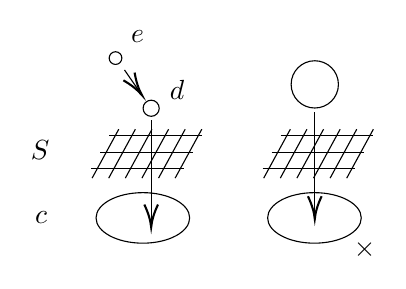
\begin{tikzpicture}[x=0.75pt,y=0.75pt,yscale=-1,xscale=1]
%uncomment if require: \path (0,300); %set diagram left start at 0, and has height of 300

%Shape: Ellipse [id:dp10401378338786049] 
\draw   (74,113.39) .. controls (74,106.67) and (84.1,101.22) .. (96.56,101.22) .. controls (109.01,101.22) and (119.11,106.67) .. (119.11,113.39) .. controls (119.11,120.11) and (109.01,125.56) .. (96.56,125.56) .. controls (84.1,125.56) and (74,120.11) .. (74,113.39) -- cycle ;
%Shape: Grid [id:dp09583060841478219] 
\draw  [draw opacity=0] (81.95,70.67) -- (126.56,70.67) -- (113.72,94.22) -- (69.11,94.22) -- cycle ; \draw   (84.95,70.67) -- (72.11,94.22)(92.95,70.67) -- (80.11,94.22)(100.95,70.67) -- (88.11,94.22)(108.95,70.67) -- (96.11,94.22)(116.95,70.67) -- (104.11,94.22)(124.95,70.67) -- (112.11,94.22) ; \draw   (80.31,73.67) -- (124.92,73.67)(75.95,81.67) -- (120.56,81.67)(71.59,89.67) -- (116.2,89.67) ; \draw    ;
%Shape: Circle [id:dp31189924819685966] 
\draw   (80.33,36.39) .. controls (80.33,34.7) and (81.7,33.33) .. (83.39,33.33) .. controls (85.08,33.33) and (86.44,34.7) .. (86.44,36.39) .. controls (86.44,38.08) and (85.08,39.44) .. (83.39,39.44) .. controls (81.7,39.44) and (80.33,38.08) .. (80.33,36.39) -- cycle ;
%Straight Lines [id:da12935033787340267] 
\draw    (87.72,42.11) -- (94.97,52.58) ;
\draw [shift={(96.11,54.22)}, rotate = 235.29] [color={rgb, 255:red, 0; green, 0; blue, 0 }  ][line width=0.75]    (10.93,-3.29) .. controls (6.95,-1.4) and (3.31,-0.3) .. (0,0) .. controls (3.31,0.3) and (6.95,1.4) .. (10.93,3.29)   ;
%Shape: Circle [id:dp7222065551952845] 
\draw   (96.67,60.56) .. controls (96.67,58.41) and (98.41,56.67) .. (100.56,56.67) .. controls (102.7,56.67) and (104.44,58.41) .. (104.44,60.56) .. controls (104.44,62.7) and (102.7,64.44) .. (100.56,64.44) .. controls (98.41,64.44) and (96.67,62.7) .. (96.67,60.56) -- cycle ;
%Straight Lines [id:da7276461675375434] 
\draw    (100.56,66.44) -- (100.56,115.89) ;
\draw [shift={(100.56,117.89)}, rotate = 270] [color={rgb, 255:red, 0; green, 0; blue, 0 }  ][line width=0.75]    (10.93,-3.29) .. controls (6.95,-1.4) and (3.31,-0.3) .. (0,0) .. controls (3.31,0.3) and (6.95,1.4) .. (10.93,3.29)   ;
%Shape: Ellipse [id:dp12697611260252684] 
\draw   (156.67,113.39) .. controls (156.67,106.67) and (166.77,101.22) .. (179.22,101.22) .. controls (191.68,101.22) and (201.78,106.67) .. (201.78,113.39) .. controls (201.78,120.11) and (191.68,125.56) .. (179.22,125.56) .. controls (166.77,125.56) and (156.67,120.11) .. (156.67,113.39) -- cycle ;
%Shape: Grid [id:dp9936460967678797] 
\draw  [draw opacity=0] (164.61,70.67) -- (209.22,70.67) -- (196.39,94.22) -- (151.78,94.22) -- cycle ; \draw   (167.61,70.67) -- (154.78,94.22)(175.61,70.67) -- (162.78,94.22)(183.61,70.67) -- (170.78,94.22)(191.61,70.67) -- (178.78,94.22)(199.61,70.67) -- (186.78,94.22)(207.61,70.67) -- (194.78,94.22) ; \draw   (162.98,73.67) -- (207.59,73.67)(158.62,81.67) -- (203.23,81.67)(154.26,89.67) -- (198.87,89.67) ; \draw    ;
%Shape: Circle [id:dp838751100400853] 
\draw   (168,49.06) .. controls (168,42.77) and (173.1,37.67) .. (179.39,37.67) .. controls (185.68,37.67) and (190.78,42.77) .. (190.78,49.06) .. controls (190.78,55.35) and (185.68,60.44) .. (179.39,60.44) .. controls (173.1,60.44) and (168,55.35) .. (168,49.06) -- cycle ;
%Straight Lines [id:da5932706956135338] 
\draw    (179.39,62.44) -- (179.39,111.89) ;
\draw [shift={(179.39,113.89)}, rotate = 270] [color={rgb, 255:red, 0; green, 0; blue, 0 }  ][line width=0.75]    (10.93,-3.29) .. controls (6.95,-1.4) and (3.31,-0.3) .. (0,0) .. controls (3.31,0.3) and (6.95,1.4) .. (10.93,3.29)   ;

% Text Node
\draw (43.33,109) node [anchor=north west][inner sep=0.75pt]   [align=left] {$\displaystyle c$};
% Text Node
\draw (41.33,75) node [anchor=north west][inner sep=0.75pt]   [align=left] {$\displaystyle S$};
% Text Node
\draw (113,123.67) node [anchor=north west][inner sep=0.75pt]   [align=left] {$\displaystyle \checkmark$};
% Text Node
\draw (197,123) node [anchor=north west][inner sep=0.75pt]   [align=left] {$\displaystyle \times $};
% Text Node
\draw (108.33,46) node [anchor=north west][inner sep=0.75pt]   [align=left] {$\displaystyle d$};
% Text Node
\draw (89.67,22) node [anchor=north west][inner sep=0.75pt]   [align=left] {$\displaystyle e$};


\end{tikzpicture}
    \end{center}

    % 这里, 我们认为指向 $c$ 的态射越复合就越小. 回忆环是一个对象的 $\mathsf {Ab}$-充实范畴, 那么其中的筛正是环的右理想; 筛的大小观念类似于 $p$-进度量下的整数越乘越小.

    一个筛越细, 能 ``通过'' 它的东西就越少, 这解释了\emph{细化}的含义; 反之, 所有东西都能通过的筛就是最粗的筛.
\end{remark}

\begin{example}
	[label={sieve-in-poset}]
	{(偏序集中的筛)}
	对于偏序集 $P$ 的元素 $p$, 记 $\downarrow p = \{x\in P\mid x\leq p\}$. 那么 $p$ 上的一个筛 $S$ 即是 $\downarrow p$ 的子集, 使得若 $x\in S$, $y\leq x$, 则 $y\in S$. 称这样的 $S$ 为 $\downarrow p$ 的\emph{向下封闭子集}.
\end{example}

\begin{example}
	[label={sieve-from-cover}]
	{(覆盖产生筛)}
	设 $X$ 为拓扑空间, $\{U_i\}$ 是其中开集 $V$ 的一个开覆盖. 那么
	$$
	\big\{W\subset V \mid \exists i, W \subset U_i\big\}
	$$
	构成 $\operatorname{Open}(X)$ 中 $V$ 上的一个筛. 直观上每个 $U_i$ 是筛上的一个 ``洞'', 比它小的对象能 ``通过'' 这个筛.
\end{example}

\begin{prop}
	[label={sieve-and-subfunctor}]
    {(筛与子函子)}
    范畴 $\mathcal C$ 的对象 $c$ 上的筛自然地一一对应于 $\yo(c)$ 的子函子.
\end{prop}

\begin{proof}
    设 $S$ 是 $c$ 上的筛, 那么
    $$
    X\colon \mathcal C^{\op}\to\mathsf {Set},\,X(d) := \{f\colon d\to c \mid f\in S\} \subset \operatorname{Hom}_{\mathcal C}(d,c) = \yo(c)(d)
    $$
    构成 $\yo(c)$ 的子函子.
    设 $X \to \yo(c)$ 为子函子, 那么
    $$
    S:=\big\{
        f \colon d\to c \mid f\in X(d)
    \big\}
    $$
    是 $c$ 上的筛. 很明显, 这两个对应是互逆的.
    注意 $X$ 的函子性恰好等价于筛 $S$ 为右理想.
    容易验证筛 $S$ 沿态射 $f\colon d\to c$ 的拉回等同于 $\yo(c)$ 的子对象 $X$ 沿 $f\colon \yo(d)\to \yo(c)$ 的拉回.
\end{proof}

在后文中, 我们将自由地运用上述对应, 将 $c$ 上的筛与 $\yo(c)$ 的子函子完全等同, 请读者务必熟悉.

%\begin{remark}
%    {}
%    若将 $\widehat {\mathcal C}$ 的对象称作 $\mathcal C$ 的 ``广义对象'', 那么 $\yo(c)$ 的子函子可称作 $c$ 的 ``广义子对象''.
%
%    $\mathcal C$ 的 ``广义对象'' $X$ 的子对象, 根据命题 \ref{subfunctor-description} 的描述, 也可视为 $X$ 上的 ``筛''.
%\end{remark}

\begin{example}
	[label={principal-sieve}]
	{(主筛)}
	对于范畴 $\mathcal C$ 中的态射 $f\colon c'\to c$,
	所有穿过 $f$ 的态射 $c''\to c'\overset{f}{\to} c$ 构成 $c$ 上的一个筛 $\downarrow f$, 称为\emph{主筛} (principal sieve).
	这类似于环的主理想.
	$\downarrow f$ 对应的 $\yo(c)$ 的子函子恰为 $\yo(f)\colon \yo(c') \to \yo(c)$ 的像.
\end{example}

\begin{example}
	[label={sieve-from-cover-subfunctor}]
	{(覆盖产生的筛对应的子函子)}
	继续例 \ref{sieve-from-cover}, 设 $S$ 为覆盖 $\{U_i\}$ 生成的筛 (视为 $\yo(V)$ 的子函子), 那么下图是余等化子.
	\begin{equation}
		\label{sieve-coeq}
		\begin{tikzcd}[ampersand replacement=\&]
			{\coprod_{i,j}\yo(U_i\cap U_j)} \& {\coprod_i \yo(U_i)} \& S
			\arrow[shift right, from=1-1, to=1-2]
			\arrow[shift left, from=1-1, to=1-2]
			\arrow[from=1-2, to=1-3]
		\end{tikzcd}
	\end{equation}
	这是因为, 由 $S$ 的定义, 对 $W\in\operatorname{Open}(X)$, 若存在 $i$, $W\subset U_i$, 则 $S(W)$ 是单元集; 否则 $S(W)$ 是空集. 由此可知下图是集合范畴中的余等化子.
	\[\begin{tikzcd}[ampersand replacement=\&, column sep=small]
		{\coprod_{i,j}\operatorname{Hom}_{\operatorname{Open}(X)}(W,U_i\cap U_j)} \& {\coprod_i \operatorname{Hom}_{\operatorname{Open}(X)}(W,U_i)} \& {S(W)}
		\arrow[shift right, from=1-1, to=1-2]
		\arrow[shift left, from=1-1, to=1-2]
		\arrow[from=1-2, to=1-3]
	\end{tikzcd}\]
	而预层的余极限是 ``逐点'' 的, 于是得 (\ref{sieve-coeq}).
	
	对 $X$ 上的任意预层 $F$, 以 $\operatorname{Hom}_{\operatorname{Presh}(X)}(-,F)$ 作用于 (\ref{sieve-coeq}), 可知下图是集合范畴中的等化子.
	\begin{equation}
		\begin{tikzcd}[ampersand replacement=\&]
			{\operatorname{Hom}_{\operatorname{Presh}(X)}(S,F)} \& {\prod_i F(U_i)} \& {\prod_{i,j}F(U_i\cap U_j)}
			\arrow[shift left, from=1-2, to=1-3]
			\arrow[shift right, from=1-2, to=1-3]
			\arrow[from=1-1, to=1-2]
		\end{tikzcd}
		\label{sieve-subfunctor-equalizer}
	\end{equation}
	因此态射集合 $\operatorname{Hom}_{\operatorname{Presh}(X)}(S,F)$ 表达了预层 $F$ 关于覆盖 $\{U_i\}$ 的下降资料 (descent data), 由覆盖 $\{U_i\}$ ``下降'' 到 $V$. 若 $F$ 为层, 就应该有 $$\operatorname{Hom}_{\operatorname{Presh}(X)}(S,F) \simeq F(V) \simeq \operatorname{Hom}_{\operatorname{Presh}(X)}(\yo(V),F).$$
\end{example}

\begin{example}
	[label={maximal-sieve}]
    {(极大筛)}
    所有指向 $c$ 的箭头的集合称为\emph{极大筛}, 也即最粗的筛.
    它对应 $\yo(c)$ 的子对象 $\yo(c)$ 自身.
    注意, $c$ 上的一个筛是极大筛当且仅当它包含 $\operatorname{id}_c$.
    设 $S$ 是 $c$ 上的筛, $f\colon d\to c$, 那么 $f\in S$ 当且仅当 $f^*S$ 为 $d$ 上的极大筛.
\end{example}

\subsubsection{预层范畴的子对象分类子}

假设 $\widehat{\mathcal C}$ 中存在子对象分类子 $\Omega$, 那么 $\Omega$ 是确定的: 由米田引理, 有自然同构
$$
\Omega(c) \simeq \operatorname{Hom}_{\widehat {\mathcal C}}(\yo(c),\Omega)
\simeq \operatorname{Sub}_{\widehat {\mathcal C}}(\yo(c))\simeq \{\text{$c$ 上的筛}\}.
$$
下面证明这个预层确实是 $\widehat{\mathcal C}$ 的子对象分类子.

\begin{prop}
	[label={presheaf-category-subobject-classifier}]
	{(预层范畴的子对象分类子)}
	在任意范畴 $\mathcal C$ 上, 定义预层 $\Omega\colon \mathcal C^{\op}\to\mathsf {Set}$, $\Omega(c) := \{\text{$c$ 上的筛}\}$, 且对态射 $f\colon d\to c$, $\Omega(f)\colon \Omega(c)\to \Omega(d)$ 为筛的拉回. 那么 $\Omega$ 是 $\widehat{\mathcal C}$ 的子对象分类子.
\end{prop}

\begin{proof}
    定义态射 $\top\colon 1 \to \Omega,$
    对每个对象 $c$ 选出 $\Omega(c)= \operatorname{Sub}_{\widehat {\mathcal C}}(\yo(c))$
    中的子对象 $\yo(c)$ 自身, 也即 $c$ 上的极大筛.
    设 $Y\to X$ 是 $\widehat{\mathcal C}$ 中的任意子对象.
    定义态射 $\chi \colon X \to \Omega$, 将 $x\in X(c)$ 对应到 $c$ 上的筛
    \begin{equation}
    	\chi_c(x) := \big\{f \colon d \to c \mid X(f)(x) \in Y(d)\big\}.
    	\tag{$\star$}
    \end{equation}
    注意 $\chi_c(x)$ 是极大筛当且仅当 $\operatorname{id}_c \in \chi_c(x)$, 也即 $x \in Y(c)$,
    所以子对象 $Y\to X$ 是如下的拉回.
    % https://q.uiver.app/#q=WzAsNCxbMCwxLCJYIl0sWzEsMSwiXFxPbWVnYSJdLFsxLDAsIjEiXSxbMCwwLCJZIl0sWzMsMF0sWzAsMSwiXFxjaGkiLDJdLFsyLDEsIlxcdG9wIl0sWzMsMl1d
    \[\begin{tikzcd}[ampersand replacement=\&]
    	Y \& 1 \\
    	X \& \Omega
    	\arrow[from=1-1, to=2-1]
    	\arrow["\chi"', from=2-1, to=2-2]
    	\arrow["\top", from=1-2, to=2-2]
    	\arrow[from=1-1, to=1-2]
    \end{tikzcd}\]
	这证明了 $\Omega$ 是 $\widehat{\mathcal C}$ 的子对象分类子, 且 $\top\colon 1\to\Omega$ 是万有子对象.
\end{proof}

\begin{remark}
	[label={presheaf-subobject-classifier-motivation}]
	{(特征函数的定义的解释)}
	假设下图中右侧方块以及长方形为拉回,
	可得左侧方块为拉回,
	% https://q.uiver.app/#q=WzAsNixbMSwwLCJZIl0sWzEsMSwiWCJdLFswLDEsIlxceW8oYykiXSxbMiwwLCIxIl0sWzIsMSwiXFxPbWVnYSJdLFswLDAsIlxcY2hpX2MoeCkiXSxbMyw0LCJcXHRvcCJdLFsxLDQsIlxcY2hpIiwyXSxbMCwzXSxbMCwxXSxbMiwxLCJ4IiwyXSxbNSwyXSxbNSwwXV0=
	\[\begin{tikzcd}[ampersand replacement=\&]
		{\chi_c(x)} \& Y \& 1 \\
		{\yo(c)} \& X \& \Omega
		\arrow["\top", from=1-3, to=2-3]
		\arrow["\chi"', from=2-2, to=2-3]
		\arrow[from=1-2, to=1-3]
		\arrow[from=1-2, to=2-2]
		\arrow["x"', from=2-1, to=2-2]
		\arrow[from=1-1, to=2-1]
		\arrow[from=1-1, to=1-2]
	\end{tikzcd}\]
	因此 $\chi_c(x) = \{f\in\yo(c)(d)\mid x\circ f\in Y(d)\}$.
	注意到对于 $x\in X(c)$, 有 $x\in Y(c)$ 当且仅当上图中存在提升 $\yo(c)\to Y$,
	当且仅当 $\chi_c(x) = \yo(c)$.
	这解释了态射 $\chi\colon X\to\Omega$ 的构造.
\end{remark}

综合上述论证, 我们得到
\begin{prop}{}
    $\widehat {\mathcal C}$ 是一个\topos{}.
\end{prop}

\begin{example}
	[label={G-set-topos}]
    {($G$-集)}
    例 \ref{G-set-presheaf-category} 介绍了 $G$-集范畴, 即 $\mathsf BG$ 上的预层范畴. 由于 $\mathsf BG$ 只有一个对象且态射均为自同构,
    其上仅有两个筛, 空集与极大筛.
    
    因此, $G$-集范畴的子对象分类子 $\Omega$ 是二元集合 $\{\top,\bot\}$, 其上带有 $G$ 的平凡作用.
    事实上, 一个 $G$-集 $X$ 的子对象 $Y$ 是其中 $G$-作用下封闭的子集. 其对应的特征函数 $X\to\{\top,\bot\}$ 就是子集 $Y$ 的特征函数.
\end{example}

%回忆\topos{}中的子对象分类子 $\Omega$ 有内蕴 Heyting 代数结构. 对于预层范畴的情形, 其结构态射可用筛具体写出.

%\begin{prop}
%	{}
%	设 $R,S$ 是范畴 $\mathcal C$ 对象 $c$ 上的筛, 即 $\Omega(c)$ 的元素.
%	\begin{itemize}
%		\item 
%		$R\land S$
%	\end{itemize}
%\end{prop}

\section{景}

\philoquote{Attempting to define a ``Weil cohomology'' with the formal properties 
necessary to establish the Weil conjectures, Grothendieck discovered \'etale 
cohomology, a fusion of ordinary sheaf cohomology and Galois cohomology. The definition required an extension of the concept of sheaf to the idea 
of a sheaf on a site --- a category equipped with an a priori notion of covering.}{Andr\'e Joyal, Myles Tierney, \cite{EGG}}

Grothendieck 意识到, 层的概念所需的关键信息是一个对象 $U$ 何时被一族进入 $U$ 的态射 (甚至不一定是 $U$ 的子对象) 所\emph{覆盖}.

\subsection{从覆盖到 Grothendieck 拓扑}

本小节有许多的定义, 在读者看来这些定义可能有些冗余. 这或许是历史的遗留, 但每个定义有各自的长处.

\begin{definition}{(覆盖结构)}
    范畴 $\mathcal C$ 上的一个\emph{覆盖结构} (coverage) $T$ 是如下资料: 对每个对象 $c$ 指定一个集合 $T(c)$, 其元素为态射族 $\{f_i \colon c_i \to c\}_{i\in I}$, 称为 $c$ 的 $T$-\emph{覆盖族} (covering family), 满足
    \begin{itemize}
    	\item (拉回下的稳定性) 若 $\{f_i \colon c_i \to c\}_{i\in I}\in T(c)$, 对任意态射 $g \colon d \to c$,
    	存在 $\{h_j \colon d_j \to d\}_{j\in J}\in T(d)$
    	使得每个 $gh_j$ 都穿过某个 $f_i$.
    \end{itemize}
	
    %带有覆盖结构的范畴 $(\mathcal C,T)$ 称为\emph{景} (site).
    对于两个覆盖结构 $T,T'$, 若 $T\subset T'$, 则称 $T'$ 较\emph{细} (fine).
\end{definition}

\begin{remark}
	{(具有拉回的范畴上的覆盖结构)}
	对于具有拉回的范畴 $\mathcal C$, 我们通常要求覆盖结构满足如下更强的条件.
	\begin{itemize}
		\item (拉回下的稳定性) 若 $\{f_i \colon c_i \to c\}_{i\in I}\in T(c)$, $g \colon d \to c$,
		则 $\{g^*(f_i) \colon d_i \to d\}_{i\in I}\in T(d)$.
	\end{itemize}
\end{remark}

%对于拓扑空间的开集范畴, 拉回下的稳定性相当于若一族开集覆盖了 $U$, 那么它们也覆盖了 $U$ 的任何子集.

%\begin{remark}{}
%    上面定义的覆盖结构有时也称为范畴上的 \emph{Grothendieck 拓扑}, 但这个词的含义有时要窄一些.
%\end{remark}

\begin{definition}
	[label={sheaf-condition}]
	{(关于态射族的层条件)}
	设 $F$ 是范畴 $\mathcal C$ 上的预层. 设 $M = \{f_i\colon c_i\to c\}_{i\in I}$ 是 $\mathcal C$ 中的一族共终点的态射. 称 $F$ 满足关于 $M$ 的\emph{层条件}, 是指对任意一组相容的元素 $(s_i\in F(c_i))_{i\in I}$,
	存在唯一的 $s\in F(c)$ 满足 $$F(f_i)(s)=s_i\,\forall i\in I.$$
	其中, 一组元素 $(s_i\in F(c_i))_{i\in I}$ \emph{相容}是指对任意态射 $f\colon d \to c_i$, $g\colon d \to c_j$, 有 $$F(f)(s_i) = F(g)(s_j) \in F(d).$$
	
	若将上面的 ``存在唯一'' 改为 ``存在至多一个'', 得到的条件称为\emph{分离性}条件.
	
	在 $\mathcal C$ 具有拉回的条件下, 层条件可简洁地表述为如下等化子,
	% https://q.uiver.app/#q=WzAsMyxbMCwwLCJGKGMpIl0sWzEsMCwiXFxwcm9kX3tpfSBGKGNfaSkiXSxbMiwwLCJcXHByb2Rfe2ksan0gRihjX2lcXHRpbWVzX2MgY19qKSJdLFsxLDIsIiIsMCx7Im9mZnNldCI6LTF9XSxbMSwyLCIiLDIseyJvZmZzZXQiOjF9XSxbMCwxXV0=
	\[\begin{tikzcd}[ampersand replacement=\&]
		{F(c)} \& {\prod_{i} F(c_i)} \& {\prod_{i,j} F(c_i\times_c c_j).}
		\arrow[shift left, from=1-2, to=1-3]
		\arrow[shift right, from=1-2, to=1-3]
		\arrow[from=1-1, to=1-2]
	\end{tikzcd}\]

	
	设 $S\to \yo(c)$ 是 $\{f_i\colon c_i\to c\}_{i\in I}$ 生成的筛对应的子函子 (命题 \ref{sieve-and-subfunctor}), 那么一组相容的元素等同于自然变换 $S\to F$,	从而层条件等价于自然变换 $S\to F$ 唯一地穿过 $\yo(c)$, 也即如下映射是同构.
	$$
	\operatorname{Hom}_{\widehat {\mathcal C}}(\yo(c),F) \to \operatorname{Hom}_{\widehat {\mathcal C}}(S,F)
	$$
	(分离性条件等价于它是单射.) 对比例 \ref{sieve-from-cover-subfunctor} 中的式 (\ref{sieve-subfunctor-equalizer}).
	$F$ 关于 $S$ 的层条件也可表述为 $F$ 是关于 $S\to \yo(c)$ 的\emph{局部对象} (定义 \ref{local-objects}), 这种表述的优势在于能一字不改地推广为 Lawvere--Tierney 拓扑的层条件 (定义 \ref{Lawvere--Tierney-topology-sheaf}).
\end{definition}

\begin{definition}
	{(关于覆盖的层条件)}
	设 $F$ 是范畴 $\mathcal C$ 上的预层. 设 $T$ 是范畴 $\mathcal C$ 上的覆盖结构. 称 $F$ 满足关于 $T$ 的\emph{层条件}就是指 $F$ 满足关于其中每个态射族的层条件.
\end{definition}

\begin{remark}
	{(覆盖结构的粗细)}
	由定义, 覆盖结构越\emph{细}, 对应的层条件就越\emph{强}, 层就越\emph{少}. 注意, 覆盖结构的粗细与筛的粗细是两个不同的概念. 对于覆盖结构 $T\subset T'$, 我们称 $T'$ 较细; 对于筛 $S\subset S'$, 我们称 $S$ 较细 (见注 \ref{sieve-intuition}).
\end{remark}

\begin{definition}
	{(层范畴)}
	设 $T$ 是范畴 $\mathcal C$ 上的覆盖结构. 定义\emph{层范畴} $\operatorname{Sh}(\mathcal C,T)$ 为 $\widehat {\mathcal C}$ 中满足关于 $T$ 的层条件的预层构成的全子范畴.
\end{definition}

``覆盖结构'' 是从 \emph{Grothendieck 拓扑}的概念中分离出的一个比较重要的条件. Grothendieck 拓扑的完整概念如下.

\begin{definition}
	[label={Grothendieck-topology}]
	{(Grothendieck 拓扑)}
	范畴 $\mathcal C$ 上的一个 \emph{Grothendieck 拓扑} (或 Grothendieck 覆盖结构) $J$ 是如下结构: 对每个对象 $c$ 指定一个集合 $J(c)$, 其元素为 $c$ 上的\emph{筛}, 称为\emph{覆盖筛} (covering sieve), 满足
	\begin{enumerate}[(1)]
		\item (极大筛) 任何对象 $c$ 上的极大筛 (定义 \ref{maximal-sieve}) 属于 $J(c)$;
		\item (拉回下的稳定性) 若 $S\in J(c)$, $f \colon d \to c$,
		则 $f^*S\in J(d)$.
		\item (传递性) 若 $S\in J(c)$, $R$ 是 $c$ 上的另一个筛, 使得对任意 $(f\colon d\to c)\in S$, 都有 $f^*R\in J(d)$, 那么 $R\in J(c)$.
	\end{enumerate}
\end{definition}

注意由定义可得对 $c$ 上的两个筛 $S\subset R$, 若 $S\in J(c)$, 则 $R\in J(c)$.
此外, 两个覆盖筛的交仍是覆盖筛.

\begin{propdef}
	[label={sieve-cover-arrow}]
	{(筛对态射的覆盖, Grothendieck 拓扑的等价条件)}
	固定范畴 $\mathcal C$ 上的 Grothendieck 拓扑 $J$, 我们称一个对象 $c$ 上的筛 $S$ \emph{覆盖}态射 $f\colon d\to c$ 是指 $f^*S\in J(d)$.
	例如 $S$ 覆盖 $\operatorname{id}_c$ 就是说 $S$ 覆盖 $c$.
	此时 Grothendieck 拓扑的条件等价于如下的形式.
	\begin{enumerate}[(1')]
		\item 筛 $S$ 覆盖它的所有元素;
		\item 若 $S$ 覆盖 $f$, 则 $S$ 也覆盖 $fg$ (只要 $f,g$ 可复合);
		\item (传递性) 若 $S$ 覆盖 $f$, $R$ 覆盖 $S$ 的每个元素, 则 $R$ 覆盖 $f$.
	\end{enumerate}
\end{propdef}

\begin{proof}
	~
	\begin{itemize}
		\item $\text{(1)(2)(3)} \Rightarrow \text{(1')(2')(3')}$.
		(1')(2') 是直接的; 只有 (3') 需要稍微说明.
		假设 $S$ 覆盖 $f\colon d\to c$ (即 $f^*S\in J(d)$) 且 $R$ 覆盖 $S$ 的每个元素. 对任意 $g\in f^*S$, 有 $fg\in S$, 从而 $R$ 覆盖 $fg$, $f^*R$ 覆盖 $g$.
		由 (3), $f^*R\in J(d)$.
		\item $\text{(1')(2')(3')} \Rightarrow \text{(1)(2)(3)}$. 只需要考虑 $\operatorname{id}_c$ 即可.
	\end{itemize}
\end{proof}

对于拓扑空间的开集范畴, ``极大筛是覆盖'' 相当于任何开集 $U$ 都覆盖了自己; 传递性相当于若一族开集覆盖了 $U$ 的每个局部, 那么它们也覆盖了 $U$.

%筛 $S$ 覆盖态射 $f\colon d\to c$ 在直观上说的是 $S$ 覆盖了 $f$ 的像 (不一定是范畴论意义下的像).

\begin{remark}
	[label={saturation-condition-covering}]
	{(关于饱和性条件)}
	Grothendieck 拓扑的定义中, 要求覆盖族是筛且满足\emph{极大筛}和\emph{传递性}的条件, 这些都是\emph{饱和性条件} (saturation condition), 假设一个覆盖结构不满足这些条件, 我们也可以关于这些条件取 ``闭包'' 而不影响层条件:
	\begin{itemize}
		\item (筛) 一族态射 $M= \{f_i\colon c_i \to c\}_{i\in I}$ 的层条件等价于其生成的筛的层条件;
		\item (极大筛) 极大筛的层条件是平凡的 (一族态射只要包含了 $\operatorname{id}_c$, 其层条件就是平凡的);
		\item (传递性) 若预层 $F$ 满足 $\{f_i\colon c_i\to c\}_{i\in I}$ 的层条件, 且对每个 $i$ 都有一族态射 $\{h_{ij}\colon c_{ij}\to c_i\}_{j\in I_i}$ 使得 $F$ 满足其层条件, 那么 $F$ 也满足复合态射族 $\{f_i\circ h_{ij}\colon c_{ij}\to c\}_{i\in I,j\in I_i}$ 的层条件. (见 Elephant \cite{Elephant} C2.1 节引理 7.)
	\end{itemize}
	因此在 Grothendieck 拓扑的定义中只有\emph{拉回下的稳定性}是关键的.
\end{remark}

\begin{prop}
	[label={sieve-and-sheaf-condition}]
	{(筛与层条件的关系)}
	\begin{enumerate}[(1)]
		\item 设 $R, S$ 是 $c$ 上的筛. 若预层 $F$ 满足关于 $R$ 的层条件, 且 $R\subset S$, 则 $F$ 也满足关于 $S$ 的层条件.
		\item 设 $R, S$ 是 $c$ 上的筛. 若预层 $F$ 满足关于 $R$ 的层条件, 且对任意 $f\in R$, $F$ 满足关于 $f^*S$ 的层条件, 则 $F$ 也满足关于 $S$ 的层条件.\label{sieve-transitive-sheaf-condition}
	\end{enumerate}
\end{prop}
\begin{proof}
	~
	\begin{enumerate}
		[(1)]
		\item 任意态射 $S\to F$ 复合 $R\hookrightarrow S$ 得到 $R\to F$, 从而唯一地延拓为 $\yo(c) \to F$.
		\item 考虑集合 $S'= \{fh\mid f\in R, h\in f^*S\}$. 由注 \ref{saturation-condition-covering} 中关于传递性的讨论, $F$ 满足关于 $S'$ 的层条件. 而 $S'\subset S$, 故 $S'$ 生成的筛包含于 $S$; 由 (1), $F$ 满足关于 $S$ 的层条件.
	\end{enumerate}
\end{proof}

\begin{prop}
	[label={finest-topology-sheaf}]
	{}
	设 $F$ 是范畴 $\mathcal C$ 上的预层, 则 $\mathcal C$ 上存在一个最细的 Grothendieck 拓扑 $J_F$ 使得 $F$ 满足关于 $J_F$ 的层条件.
\end{prop}
\begin{proof}
	定义覆盖结构 $J_F$ 如下,
	$$
	J_F(c) = \{\text{$c$ 上的筛 $S\hookrightarrow\yo(c)$} \mid \text{对任意 $f\colon d\to c$, $F$ 满足关于 $f^*S$ 的层条件}\}.
	$$
	由定义, 对任意 Grothendieck 拓扑 $J$, 若 $F$ 为 $J$-层, 则 (由 $J$-覆盖筛的拉回稳定性) $J\subset J_F$.
	我们只需验证 $J_F$ 为 Grothendieck 拓扑.
	\begin{itemize}
		\item (极大筛) 极大筛的拉回仍是极大筛, 极大筛的层条件是平凡的, 故极大筛均属于 $J_F$.
		\item (拉回下的稳定性) 假设 $S\in J_F(c)$, $f\colon d\to c$, 由于 $f^*S$ 的拉回也是 $S$ 的拉回, 故 $f^*S\in J_F(d)$.
		\item (传递性)
		假设 $S\in J_F(c)$,
		且 $R$ 是 $c$ 上的另一个筛,
		使得对任意 $(f\colon d\to c)\in S$, $f^*R\in J_F(d)$.
		%
		%		那么对任意 $h\colon d\to c$,
		%			$F$ 满足关于 $f^*S$ 的层条件,
		%			且对任意 $g\colon e\to d$,
		%			$F$ 满足关于 $g^*f^*R$ 的层条件.
		%
		%由注 \ref{saturation-condition-covering} 关于传递性的讨论,
		%
		
		由 $S\in J_F(c)$, 对任意 $h\colon b\to c$,
		$F$ 满足 $h^*S$ 的层条件.
		
		对任意 $(k\colon a\to b)\in h^*S$, $(hk\colon a\to c)\in S$.
		由 $R$ 的假设, $(hk)^*R = k^*h^*R\in J_F(a)$; 特别地, $F$ 满足关于 $k^*h^*R$ 的层条件.
		
		由以上结论及命题 \ref{sieve-and-sheaf-condition} (\ref{sieve-transitive-sheaf-condition}),
		$F$ 满足关于 $h^*R$ 的层条件.
		%
		这说明 $R\in J_F(c)$.
	\end{itemize}
\end{proof}

\begin{prop}
	[label={coverage-generated-Grothendieck-topology}]
	{(覆盖与 Grothendieck 拓扑的关系)}
	设范畴 $\mathcal C$ 上有覆盖结构 $T$. 那么存在 Grothendieck 拓扑 $J$ 给出与 $T$ 相同的层条件.
%	具体地,
%	$$
%	J(c)=\{\text{$c$ 上的筛 $S$} \mid \cdots\}.
%	$$
%	\todo{}
\end{prop}
\begin{proof}
	令 $\overline{T}$ 为 $T$ 中的覆盖族生成的筛的集合, 
	则 $T$ 的层条件等价于 $\overline{T}$ 的层条件.
	令 $J$ 为所有包含 $\overline{T}$ 的 Grothendieck 拓扑的交, 则 $J$ 为 Grothendieck 拓扑. ($J$ 的表达式可显式写出, 此处略去.)
	设 $F$ 为 $T$-层. 由命题 \ref{finest-topology-sheaf} 的证明, $\overline{T}\subset J_F$, 从而 $J\subset J_F$.
	这说明 $F$ 为 $J$-层. 故 $J$ 给出与 $T$ 相同的层条件.
	%\todo{}sieve-and-sheaf-condition
\end{proof}

\begin{remark}
	{}
	一般而言, 即使覆盖结构很简洁, 也难以根据命题 \ref{coverage-generated-Grothendieck-topology} 具体写出对应的 Grothendieck 拓扑. 覆盖结构与 Grothendieck 拓扑的关系正如一个群的生成元和群本身的关系.
\end{remark}

下面这个概念也被某些文献用作 Grothendieck 拓扑的定义.

\begin{definition}
	{(Grothendieck 拓扑基)}
	设范畴 $\mathcal C$ 有拉回. 其上的一组 \emph{Grothendieck 拓扑基} (basis for a Grothendieck topology, 又称 \emph{Grothendieck 预拓扑}, pretopology) $K$ 是如下结构:
	对每个对象 $c$ 指定一个集合 $K(c)$, 其元素为态射族 $\{f_i\colon c_i\to c\}_{i\in I}$, 满足
	\begin{itemize}
		\item (恒等) $\{\operatorname{id}_c\} \in K(c)$;
		\item (拉回下的稳定性) 若 $\{f_i\colon c_i\to c\}_{i\in I} \in K(c)$, $g\colon d\to c$, 则 $\{g^*f_i\}_{i\in I}\in K(d)$;
		\item (传递性) 若 $\{f_i\colon c_i\to c\}_{i\in I} \in K(c)$, 且对每个 $i\in I$, 有 $\{g_{ij}\colon d_{ij}\to c_i\}_{j\in I_i} \in K(c_i)$, 则 $\{f_i\circ g_{ij}\colon d_{ij}\to c\}_{i\in I,j\in I_i} \in K(c)$.
	\end{itemize}
\end{definition}

\begin{definition}
	{(基生成的 Grothendieck 拓扑)}
	Grothendieck 拓扑基 $K$ \emph{生成}的 Grothendieck 拓扑 $J$ 如下:
	$$
	J(c) = \{ \text{$c$ 上的筛 $S$} \mid \exists R\in K(c), R\subset S \}.
	$$
	为了表达的方便, 我们也将用覆盖结构或 Grothendieck 拓扑基来代指其生成的 Grothendieck 拓扑.
\end{definition}

%\begin{remark}
%	{}
%	引入\emph{覆盖结构}以及 \emph{Grothendieck 拓扑基}等概念的目的大约是
%	\begin{itemize}
%		\item 方便给出 Grothendieck 拓扑 (不需要给出所有的筛);
%		\item 方便验证层条件 (不需要对所有的筛验证).
%	\end{itemize}
%%	而 Grothendieck 拓扑的优势在于
%%	\begin{itemize}
%%		\item 唯一性 (命题 \ref{coverage-generated-Grothendieck-topology});
%%		\item 与后文介绍的 Lawvere--Tierney 拓扑 (定义 \ref{Lawvere--Tierney-topology}) 的关系.
%%	\end{itemize}
%	\emph{覆盖结构}与 Grothendieck 拓扑的关系正如一个群的生成元和群本身的关系.
%\end{remark}

\begin{definition}
	{(景)}
	带有 Grothendieck 拓扑的 (小) 范畴称为\emph{景}.
\end{definition}

\begin{definition}
	[label={convention-coverage}]
	{(Grothendieck 拓扑语境下的 ``覆盖'')}
	当范畴 $\mathcal C$ 上有 Grothendieck 拓扑 $J$ 时, 作如下约定: 称一族态射 $\{f_i\colon c_i\to c\}$ \emph{覆盖}了对象 $c$ 是指其生成的筛 $$\{h\colon d\to c\mid \text{$h$ 穿过某个 $f_i$}\}$$ 是 $J$-覆盖筛.
\end{definition}

\begin{remark}
	{(关于景的小性)}
	我们一般要求景是小的, 但是许多结论可以推广到所谓\emph{本质小}的景, 即其有一个小的 $J$-稠密子范畴 (定义 \ref{site-J-dense-subcategory}).
\end{remark}



\subsection{常见的景}

% 正如环中一族元素可以生成一个右理想, 范畴 $\mathcal C$ 中一族指向 $U$ 的箭头也可以生成一个筛. 容易看到, 将覆盖族替换为生成的筛, 不影响层的概念 (正如将环中的一族元素替换为其生成的理想, 不影响对应谱上的闭集一样). 因此我们不妨考虑仅由筛构成的覆盖结构.

\begin{example}
	{}
	每个范畴 $\mathcal C$ 都构成一个平凡的景, 其上的覆盖结构为空.
	该覆盖结构对应的 Grothendieck 拓扑称为\emph{平凡拓扑} $J_{\text{平凡}}$, 其中仅包含每个对象上的极大筛.
	一族态射 $\{f_i\colon c_i\to c\}$ 覆盖 $c$ 当且仅当某个 $f_i$ 穿过 $\operatorname{id}_c$, 即 $f_i$ 为收缩.
	由定义, 这个景上的层是 $\mathcal C$ 上的预层.
\end{example}

\begin{example}
    [label={topological-space-as-site}]
    {(拓扑空间)}
    拓扑空间 $X$ 的开集范畴 $\operatorname{Open}(X)$ 构成一个景, 其上的覆盖结构是\emph{开覆盖}.
    注意此时 ``拉回下的稳定性'' 即是说若一族开集 $\{U_i\}$ 覆盖了 $V$, 那么对于 $W\subset V$, $\{U_i\land W\}$ 覆盖了 $W$.
    %因为每个可表函子 $\yo(U)$ 都是层, 所以这个覆盖结构定义的 Grothendieck 拓扑是次典范的.
\end{example}

%\todo{解释景的小性}

\begin{example}
    {(拓扑空间范畴)}
    拓扑空间的范畴\footnotemark{}上有一个由\emph{开覆盖}确定的覆盖结构.
\end{example}

\footnotetext{$\mathsf {Top}$ 不是小范畴, 因为每个集合都能配上离散拓扑成为一个拓扑空间. 但是出于实用的目的, 我们可以考虑其中小的子范畴, 如可分 Hausdorff 空间范畴 (回忆, 可分空间是指有可数稠密子集的空间).}

\begin{example}
	[label={locale-as-site}]
    {(位象)}
    % 定义\emph{位象}是一个偏序集 $A$, 存在有限交与任意并 (若将偏序集视为范畴, 这个条件就是说存在有限极限与任意余极限), 且满足分配律
    % $$a \wedge \bigvee_{i\in I} b_i = \bigvee_{i\in I} (a\wedge b_i)\,(\forall a,b_i\in A),$$
    % 其中 $I$ 是任意集合.
    % 位象的态射 $A\to B$ 是偏序集的\emph{反向}态射 $B\to A$ (想象开集的拉回), 保持有限交与任意并.
    
    对于\fm{} $A$, 将其视为范畴, 我们定义 $A$ 上的覆盖结构:
    当一族态射 $\{U_i \to U\}_{i\in I}$ 满足 $U = \bigvee_{i\in I} U_i$ 时, 称其为覆盖族.
    由此, 每个位象都 (反变地) 对应一个景.
\end{example}

\begin{example}
    [label={cartsp-site}]
    {(Cartesius 空间)}
    考虑 Cartesius 空间\footnotemark{}的范畴 $\mathsf {CartSp}$, 其中的对象为 $\mathbb{R}^0,\mathbb{R}^1,\mathbb{R}^2,\cdots$,
    态射为光滑映射.
    称 $\mathbb{R}^n$ 的开覆盖 $\{U_i\}$ 为 \emph{好覆盖} (good cover) 是指 $U_i$ 同胚于 $\mathbb{R}^n$, 且任意有限个 $U_i$ 的交 (假若非空) 都同胚于 $\mathbb{R}^n$.
    这给出了 $\mathsf {CartSp}$ 上的一个覆盖结构, 称之为 \emph{Cartesius 空间景}.
    Cartesius 空间景上的层称作\emph{光滑空间} (smooth space), 记 $\mathsf {SmoothSp}$ 为光滑空间的范畴.
    
    记 $\mathsf {Man}$ 为 (光滑) 流形的范畴. 光滑空间是光滑流形的推广: 对于流形 $M$, 定义光滑空间 $$\underline{M}\colon \mathsf {CartSp}^\op\to\mathsf {Set},\ \mathbb{R}^n\mapsto \operatorname{Hom}_{\mathsf {Man}}(\mathbb{R}^n,M),$$
    这给出了嵌入 $\mathsf {Man}\to \mathsf {SmoothSp}$.
    光滑空间是\emph{广义微分几何} (diffeology) 的研究对象. 在量子场论中, 由于人们常常需要考虑 ``场的空间'' (例如两个流形之间的映射的空间), 操作其上的微分形式, 而它们不是传统意义上的流形, 故使用光滑空间的概念能够更清晰地显示几何意义. 参见 Fr\'ed\'eric Paugam \cite{MQF} 第 3 章.
    
    对于光滑空间 $X\colon \mathsf {CartSp}^\op\to\mathsf {Set}$, $X(\mathbb{R}^n)$ 是 ``$\mathbb{R}^n$ 到 $X$ 的光滑映射的集合'' (这不过是米田引理), 也即空间 $X$ 上 $n$ 维 ``广义坐标系'' 的集合. 层条件表示的是 ``广义坐标系'' 的\emph{粘合条件}, 即当 $\mathbb{R}^n=\bigcup U_i$ 为好覆盖时, 一族相容的广义坐标系 $U_i\to X$ 可粘合为广义坐标系 $\mathbb{R}^n\to X$.
    
    一个重要的光滑空间是 ``微分形式的模空间'' $\Omega^k$, 它作为 $\mathsf {CartSp}$ 上的预层将 $\mathbb{R}^n$ 对应到其上 $k$-形式的集合 $\Omega^k(\mathbb{R}^n)$. 称其为微分形式的模空间是因为, 对任意流形 $M$ 有自然同构
    \[\operatorname{Hom}_{\mathsf {SmoothSp}}(\underline{M},\Omega^k) \simeq \Omega^k(M).\]
    容易验证 $\Omega^k$ 满足层条件, 即对于 $\mathbb{R}^n$ 的好覆盖 $\{U_i\}$, 每个 $U_i$ 上相容的微分形式可以给出 $\mathbb{R}^n$ 整体上的微分形式.
\end{example}

\footnotetext{注. Cartesius 是法国数学家 Ren\'e Descartes (``笛卡尔'') 的姓氏的拉丁化写法. %这里的 $\mathbb{R}^n$ 起到的作用正合 Descartes 的原意, 即给出空间的一部分上的坐标.
}

\begin{example}
	{(超几何)}
	$\mathbb{Z}/2\mathbb{Z}$-分次向量空间范畴有一个对称幺半范畴结构, 其交换同构 $V\otimes W\to W\otimes V$ 在奇部分的作用为 $v\otimes w\mapsto -w\otimes v$. 关于此对称幺半范畴结构的交换代数称为\emph{超交换代数}\footnotemark{}. 超几何是超交换代数对应的几何, 是一些量子场论 (如超对称场论, 超引力) 使用的语言.
	考虑范畴 $\mathsf {SupCartSp}$ (超 Cartesius 空间), 其对象 $\mathbb{R}^{n|q} = \mathbb{R}^n\times\mathbb{R}^{0|q}$ 是 ``有 $n$ 个偶坐标和 $q$ 个奇坐标'' 的空间 (物理学家所使用的术语), 即超交换代数
	$C^\infty (\mathbb{R}^n)\otimes \wedge^\bullet (\mathbb{R}^q)^*$
	的形式对偶.
	
	定义 $\mathsf {SupCartSp}$ 上的覆盖结构 $\{\iota_i\times\operatorname{id}\colon U_i\times \mathbb{R}^{0|q}\to\mathbb{R}^{n}\times\mathbb{R}^{0|q}\}$, 其中 $\{\iota_i\colon U_i\to\mathbb{R}^n\}$ 构成 $\mathbb{R}^n$ 的好覆盖.
	于是 $\mathsf {SupCartSp}$ 成为一景, 其上的层称作\emph{超光滑空间} (super smooth space).
	Urs Schreiber \cite{HTTP} 介绍了物理中旋量场等结构用超几何语言的表述, 以及其它对象在\topos{}理论中的表述.
\end{example}
\footnotetext{对超几何与量子场论感兴趣的读者可阅读 IAS 的讲义 \cite{QFT}.}

\begin{example}
    [label={zariski-site}]
    {(Zariski 景)}
    %固定环 $k$,
    考虑\emph{有限表现} (finitely presented) 环 (形如 $\mathbb{Z}[x_1,\cdots,x_n]/(f_1,\cdots,f_m)$ 的环) 的范畴 $\mathsf {Ring}_{\text{fp}}$. 这是一个小范畴\footnotemark.
    考虑其对偶范畴 $\mathsf {Ring}_{\text{fp}}^{\op}$, 也即仿射概形的范畴.
    对于环 $A$, 我们记 $\operatorname{Spec} A \in \mathsf {Ring}_{\text{fp}}^{\op}$ 为 $A$ 在对偶范畴中的化身.

    回忆, Zariski 拓扑的标准开集 (但不一定是全部的开集) 形如 $\operatorname{Spec} A_f \to \operatorname{Spec}A$, 也即局部化的环同态 $A \to A_f$. 若 $n$ 个元素 $f_1,\cdots,f_n \in A$ 生成了单位理想 $(1)$ ($f_1,\cdots,f_n$ 构成了 $\operatorname{Spec}A$ 上的 ``单位分解''),
    规定 $\{\operatorname{Spec}A_{f_i} \to \operatorname{Spec}A\}$ 构成覆盖. 这定义了 $\mathsf {Ring}_{\text{fp}}^{\op}$ 上的一个覆盖结构, 这便是 \emph{Zariski 景}.
    Zariski 景可以提供\emph{综合代数几何} (synthetic algebraic geometry) 的模型
%
    %Zariski 景上的\emph{结构层} (structure sheaf) 是遗忘函子 $\mathsf{Ring}_{\text{fp}} \to \mathsf{Set}$.
    %\todo{这个层的意义}
    %这个层与综合微分几何中的 ``直线'' 有关
    (见定义 \ref{SDG-algebraic-model}; 关于综合代数几何, 见 \cite{FSAG}).
\end{example}

\footnotetext{严格地说, 它是本质小 (essentially small) 范畴, 也即它的对象模掉同构之后构成一个集合.}

\begin{example}
	[label={small-etale-site}]
	{(平展景)}
	{\small (本例需要一些背景知识.)} 平展景是 ``拓扑空间上开集范畴'' 在代数几何中的类比. 设 $X$ 为概形, 考虑概形范畴的俯范畴 $\mathsf {Sch}_{/X}$ 中由平展映射 $U\to X$ 构成的全子范畴 $\mathsf {Sch}_{/X,\text{\'et}}$. 这称作 $X$ 上的 (小)\emph{平展景} (small \'etale site).
\end{example}

\subsection{典范与次典范拓扑}

%如下定义出自 SGA 4 \cite{SGA4} II.2 节.

\begin{propdef}
	[label={canonical-topology}]
	{(次典范和典范 Grothendieck 拓扑)}
	对于范畴 $\mathcal C$ 上的 Grothendieck 拓扑 $J$, 若以下两个等价条件之一成立, 则称之为\emph{次典范} (subcanonical) Grothendieck 拓扑:
	\begin{itemize}
		\item 对每个 $J$-覆盖筛 $S = \{f_i\colon c_i\to c\}$, 考虑 $c_i$ 之间在 $c$ 上 (也即与 $f_i$ 相容) 的所有映射, $S$ 构成该图上的余极限余锥. 这样的筛又称为\emph{有效满} (effective-epimorphic) 的.
		\item 每个可表函子 $\yo(c)$ 都是层, 也即米田嵌入 $\mathcal C\hookrightarrow\widehat {\mathcal C}$ 穿过 $\operatorname{Sh}(\mathcal C,J)$.
	\end{itemize}
	定义\emph{典范 Grothendieck 拓扑}是最细的次典范 Grothendieck 拓扑. (回忆, 称一个 Grothendieck 拓扑较细是指其中覆盖筛较多).
\end{propdef}
\begin{proof}
	设 $S$ 为 $c$ 上的筛, $S$ 是有效满的当且仅当对任意对象 $d$, 任意态射 $S\to\yo(d)$ 唯一地延拓为态射 $\yo(c) \to \yo(d)$;
	这就是说每个可表函子 $\yo(d)$ 都满足关于 $S$ 的层条件. 因此, 定义中的两个条件等价.
	
	由命题 \ref{finest-topology-sheaf}, 对每个 $c\in\mathcal C$ 存在一个使得 $\yo(c)$ 为层的最细的 Grothendieck 拓扑 $J_{\yo(c)}$.
	进而存在使得所有 $\yo(c)$ 同时为层的最细的 Grothendieck 拓扑 $\bigcap_{c\in\mathcal C} J_{\yo(c)}$. 它就是最细的次典范 Grothendieck 拓扑.
\end{proof}

\begin{example}
	{(常见的次典范 Grothendieck 拓扑)}
	\begin{itemize}
		\item 一个拓扑空间上的 Grothendieck 拓扑 (例 \ref{topological-space-as-site}) 是次典范的.
		\item Zariski 景 (例 \ref{zariski-site}) 是次典范的.
	\end{itemize}
\end{example}

\begin{example}
	{(位象上的典范拓扑)}
	位象 (\fm{}) 视为景 (例 \ref{locale-as-site}), 其上的 Grothendieck 拓扑是典范的, 因为\fm{}中一族元素的余极限是它们的并. 换言之, 位象的每个开子空间都可视为其上的层.
\end{example}

\begin{example}
	[label={canonical-topology-on-topos}]
	{(Grothendieck \topos{}上的典范拓扑)}
	一个 Grothendieck \topos{} $\operatorname{Sh}(\mathcal C,J)$ 本身也可视为一个景, 其上的典范 Grothendieck 拓扑可描述如下: 一个筛 $\{f_i\colon U_i\to X\mid i\in I\}$ 是覆盖筛当且仅当下列等价条件之一成立.
	\begin{itemize}
		\item 筛 $\{f_i\colon U_i\to X\mid i\in I\}$ 构成余极限余锥;
		\item $\bigvee_{i\in I}\operatorname{im}f_i=X$;
		\item 对任意态射 $g,h\colon X\to Y$, 若 $gf_i=hf_i\,(\forall i\in I)$, 则 $g=h$. 满足这个条件的态射族又称为\emph{联合满射族} (jointly epic family).
	\end{itemize}
%	它, 当且仅当 $\bigvee_{i\in I}\operatorname{im}f_i=X$.
%	(证明这两个条件等价是容易的. 假设一个筛 $\{f_i\colon U_i\to X\mid i\in I\}$ 构成余极限余锥, 由于每个 $f_i$ 都穿过 $\bigvee_{i\in I}\operatorname{im}f_i$, 余极限的泛性质告诉我们 $\operatorname{id}_X$ 也穿过 $\bigvee_{i\in I}\operatorname{im}f_i$. 另一方面, 假设 $\bigvee_{i\in I}\operatorname{im}f_i=X$, $gf_i$ 那么 $\operatorname{eq}$)
	
	%\todo{证明?}
	$\operatorname{Sh}(\mathcal C,J)$ 作为景, 其上的层范畴 $\operatorname{Sh}(\operatorname{Sh}(\mathcal C,J),\text{典范})$ 等价于 $\operatorname{Sh}(\mathcal C,J)$ 本身.
\end{example}

%\begin{prop}
%	{(Grothendieck \topos{}上的典范 Grothendieck 拓扑)}
%	设 $\mathcal C$ 为 Grothendieck \topos{}
%\end{prop}

\section{层化与 Grothendieck $+$构造}

%局部化是另一种等价的给出 ``范畴上的拓扑'' 的方式.

% 附录

回忆拓扑空间上一个开覆盖 $\{U_i\}$ 生成的筛 $S$ 可表示为余极限 $\operatorname{colim}\yo(U_i)$ (例 \ref{sieve-from-cover-subfunctor}). 自由余完备化 $\yo$ 不保持余极限, 而层化的效果即是使 $S\to\yo(c)$ 变为同构, \emph{层化弥补了自由余完备化所破坏的余极限}. 一种通用的将某些态射变为同构的方法是\emph{局部化} (附录 \ref{reflective-subcategory-and-localization} 节). 事实上, 层范畴是预层范畴的局部化, 而在层范畴中 $S$ 与 $\yo(c)$ 变成了同构的对象.
% 下面这一段参考 nLab,
% https://ncatlab.org/nlab/show/sheafification#ExistenceOfLeftAdjoint
%
% SGL V.3 定理 1
%
使用 Adámek 与 Rosický \cite{LPAC} 引入的可表现范畴的一般理论 (附录 \ref{appendix-presentable-categories} 节), 可以得到层范畴的一种简单描述. 层范畴 $\operatorname{Sh}(\mathcal C,J)$ 是 $\widehat {\mathcal C}$ 中关于所有 $J$-覆盖筛 $S\to\yo(c)$ 的局部对象的全子范畴. 由命题 \ref{local-object-reflective-subcategory}, $\operatorname{Sh}(\mathcal C,J)$ 是 $\widehat {\mathcal C}$ 的自反子范畴 (\cite{LPAC} 第 2 章 2D, 2E 节对此还有一种更加抽象的证明).
由命题 \ref{reflective-subcategories-are-localizations}, $\operatorname{Sh}(\mathcal C,J)$ 是 $\widehat {\mathcal C}$ 关于 $W = \{(S\to\yo(c))\in J(c)\}$ 生成的强饱和态射族 $\overline{W}$ (注 \ref{strongly-saturated-class-of-morphisms}) 的局部化.
可以证明 $\overline{W}$ 是 $W$ 关于箭头范畴中 (小) 余极限的完备化. $\overline{W}$ 中的元素形如
\[
\operatorname{colim}_i S_i \to \operatorname{colim}_i \yo(c_i).
\]
可以证明这个态射族具有右分式计算 (定义 \ref{calculus-of-fractions}),
从而 $\operatorname{Sh}(\mathcal C,J)$ 等价于分式计算给出的范畴 $\widehat {\mathcal C}[\overline{W}^{-1}]$:
\begin{equation}
	\operatorname{Hom}_{\widehat {\mathcal C}[\overline{W}^{-1}]}
	(X,Y)=\operatorname{colim}_{(X'\to X)\in\overline{W}}\operatorname{Hom}_{\widehat {\mathcal C}}(X',Y).
	\tag{$\star$}
\end{equation}
我们不会给出上述论证的全部细节 (参见 \cite{nlab:sheafification}), 而是采取另一种较具体的方式构造层化, 它被称为 \emph{Grothendieck $+$构造} (plus construction), 其与 $(\star)$ 至少在精神上是相似的.
在证明层化的性质之后, 我们几乎不会再使用 $+$ 构造; 因此知道这种构造的存在就足够了.

\begin{definition}
	[label={Grothendieck-plus-construction}]
	{(Grothendieck $+$构造)}
	设 $J$ 为范畴 $\mathcal C$ 上的 Grothendieck 拓扑, $X$ 为 $\mathcal C$ 上的预层, 定义预层 $X^+$,
	\[
	\operatorname{Hom}_{\widehat {\mathcal C}}(\yo(c),X^+) = X^+(c) := \operatorname{colim}_{(S\to \yo(c))\in J(c)}\operatorname{Hom}_{\widehat {\mathcal C}} (S,X).
	\]
	$X^+\colon \mathcal {C}^{\op}\to\mathsf {Set}$ 的函子性来自拉回稳定性: 对任意态射 $f\colon c'\to c$, 有映射
	$X^+(f)\colon X^+(c) \to X^+(c')$,
	$[S\to X]\mapsto [f^*S\to S\to X]$.
	很明显, 有典范的态射 $\eta_X\colon X \to X^+$ 将元素 $\yo(c) \to X$ 映射到 $[\yo(c) \to X]$, 并且 $\eta_X$ 关于 $X$ 有自然性, 即对于预层态射 $X\to Y$ 有交换图
	% https://q.uiver.app/#q=WzAsNCxbMCwwLCJYIl0sWzEsMCwiWSJdLFswLDEsIlheKyJdLFsxLDEsIlleKyJdLFswLDIsIlxcZXRhX1giLDJdLFsxLDMsIlxcZXRhX1kiXSxbMCwxXSxbMiwzXV0=
	\[\begin{tikzcd}[ampersand replacement=\&]
		X \& Y \\
		{X^+} \& {Y^+.}
		\arrow[from=1-1, to=1-2]
		\arrow["{\eta_X}"', from=1-1, to=2-1]
		\arrow["{\eta_Y}", from=1-2, to=2-2]
		\arrow[from=2-1, to=2-2]
	\end{tikzcd}\]
	%换言之, $\eta_F\colon F(c)\to F^+(c)$ 将 $x\in F(c)$ 映射到
\end{definition}

对于覆盖筛 $S\to \yo(c)$, $\operatorname{Hom}_{\widehat {\mathcal C}} (S,X)$ 的元素是对所有 $(f\colon d\to c)\in S$ 选取相容的一族元素 $X(d)$ (见定义 \ref{sheaf-condition}). 因此 $X^+(c)$ 的元素也可理解为 $X$ 在 $c$ 上 ``相容族'' 的等价类.
典范的映射 $\eta_X\colon X(c)\to X^+(c)$ 将 $x\in X(c)$ 映射到 $x$ 产生的相容族 $(X(f)(x))_{f\in S}$.

另一个有用的事实是, 对元素 $x\colon \yo(c)\to X^+$ 的任意代表 $S \to X$ ($S\in J(c)$),
有如下交换图.
% https://q.uiver.app/#q=WzAsNCxbMCwwLCJTIl0sWzEsMCwiWCJdLFswLDEsIlxceW8oYykiXSxbMSwxLCJYXisiXSxbMCwyLCIiLDAseyJzdHlsZSI6eyJ0YWlsIjp7Im5hbWUiOiJob29rIiwic2lkZSI6InRvcCJ9fX1dLFswLDEsImZcXG1hcHN0byB4X2YiXSxbMSwzLCJcXGV0YV9YIl0sWzIsMywieCIsMl1d
\[\begin{tikzcd}[ampersand replacement=\&]
	S \& X \\
	{\yo(c)} \& {X^+}
	\arrow[hook, from=1-1, to=2-1]
	\arrow["{f\mapsto x_f}", from=1-1, to=1-2]
	\arrow["{\eta_X}", from=1-2, to=2-2]
	\arrow["x"', from=2-1, to=2-2]
\end{tikzcd}\]
直接验证上图交换: 对任意 $(f\colon d\to c)\in S$, 有 $f^*S = \yo(d)$, 从而 $[x_f\colon \yo(d)\to X] = [f^*S \to S\to X]$.

\begin{prop}
	[label={plus-finite-limits}]
	{}
	$+$ 构造保持有限极限.
\end{prop}
\begin{proof}
	注意到余极限 $\operatorname{colim}_{(S\to \yo(c))\in J(c)}$ 的指标范畴为偏序集, 其中任意两个覆盖筛有共同的加细, 这说明该余极限为滤余极限. 结论来自滤余极限的一般性质 (命题 \ref{lambda-filtered-colimit-commutes-with-lambda-small-limit}).
\end{proof}

\begin{prop}
	{}
	在定义 \ref{Grothendieck-plus-construction} 中, $F$ 是层当且仅当 $\eta_F\colon F\to F^+$ 为同构,
	$F$ 是分离对象当且仅当 $\eta_F\colon F\to F^+$ 为单射.
\end{prop}
\begin{proof}
	由 Grothendieck $+$构造的定义以及层条件 (分离条件) 的定义即得.
\end{proof}

一次 $+$ 构造的结果 $F^+$ 不一定是层, 但下面的命题表明 $F^+$ 离层进了一步, 而 $F^{++}$ 必然是层.

%
%\begin{prop}
%	{}
%	设 $J$ 为范畴 $\mathcal C$ 上的 Grothendieck 拓扑, 则嵌入 $i\colon \text{Sh}(\mathcal C,J)\hookrightarrow \widehat {\mathcal C}$ 有左伴随 $a$, 满足
%	\[
%	a(F)(c) = \operatorname{colim}_{}
%	\]
%	\todo{}
%\end{prop}

\begin{prop}
	[label={double-plus-good}] % doubleplusgood
	{}
	对预层 $F$, $F^+$ 分离; 进一步, 当 $F$ 分离时, $F^{+}$ 是层.
\end{prop}
\begin{proof}~
%	对预层的态射 $f\colon X\to Y$, 若存在如下虚线态射, 则称 $f$ 为 ``$+$ 关联'' 的.
%	% https://q.uiver.app/#q=WzAsNCxbMCwwLCJYIl0sWzEsMCwiWSJdLFswLDEsIlheKyJdLFsxLDEsIlleKyJdLFswLDIsIlxcZXRhX1giLDJdLFswLDEsImYiXSxbMSwzLCJcXGV0YV9ZIl0sWzIsMywiZl4rIiwyXSxbMSwyLCJcXGV4aXN0cyIsMSx7InN0eWxlIjp7ImJvZHkiOnsibmFtZSI6ImRhc2hlZCJ9fX1dXQ==
%	\[\begin{tikzcd}[ampersand replacement=\&]
%		X \& Y \\
%		{X^+} \& {Y^+}
%		\arrow["{\eta_X}"', from=1-1, to=2-1]
%		\arrow["f", from=1-1, to=1-2]
%		\arrow["{\eta_Y}", from=1-2, to=2-2]
%		\arrow["{f^+}"', from=2-1, to=2-2]
%		\arrow["\exists"{description}, dashed, from=1-2, to=2-1]
%	\end{tikzcd}\]
%	首先, 由定义可以验证 $\eta_{X^+} = (\eta_X)^+$, 从而 $\eta_X$ 是 ``$+$ 关联'' 的.
	\begin{itemize}
		\item $F^+$ 分离. 设 $x_1\colon S_1\to F$, $x_2\colon S_2\to F$ ($S_1,S_2\in J(c)$) 是 $F^+(c)$ 的两个元素 (的代表),
		两者在某个覆盖 $S\in J(c)$ 上相等, 即对任意 $(f\colon d\to c)\in S$, $f^*S_1\to S_1\overset{x_1}{\to} F$ 与 $f^*S_2\to S_2\overset{x_2}{\to} F$ 代表 $F^+(d)$ 的同一个元素, 而这表示存在 $S_f\in J(d)$ 使下图交换.
		% https://q.uiver.app/#q=WzAsNixbMCwxLCJTX2YiXSxbMSwwLCJmXipTXzEiXSxbMSwyLCJmXipTXzIiXSxbMiwwLCJTXzEiXSxbMiwyLCJTXzIiXSxbMywxLCJGIl0sWzAsMiwiIiwwLHsic3R5bGUiOnsidGFpbCI6eyJuYW1lIjoiaG9vayIsInNpZGUiOiJ0b3AifX19XSxbMCwxLCIiLDIseyJzdHlsZSI6eyJ0YWlsIjp7Im5hbWUiOiJob29rIiwic2lkZSI6ImJvdHRvbSJ9fX1dLFsxLDNdLFsyLDRdLFszLDUsInhfMSJdLFs0LDUsInhfMiIsMl1d
		\[\begin{tikzcd}[ampersand replacement=\&,sep=small]
			\& {\!f^*S_1} \& {S_1} \\
			{S_f} \&\&\& F \\
			\& {\!f^*S_2} \& {S_2}
			\arrow[hook, from=2-1, to=3-2]
			\arrow[hook', from=2-1, to=1-2]
			\arrow[from=1-2, to=1-3]
			\arrow[from=3-2, to=3-3]
			\arrow["{x_1}", from=1-3, to=2-4]
			\arrow["{x_2}"', from=3-3, to=2-4]
		\end{tikzcd}\]
		由传递性, 所有 $S_f$ (与 $f$ 复合后) 构成 $c$ 的覆盖筛, 故 $x_1,x_2$ 代表了 $F^+(c)$ 的同一个元素.
		\item 假设 $F$ 分离, 我们证明 $F^+$ 为层.
		首先注意到若 $x_1\colon S_1\to F$, $x_2\colon S_2\to F$ ($S_1,S_2\in J(c)$) 代表了 $F^+(c)$ 的同一个元素,
		由于 $F$ 分离, $x_1,x_2$ 必须在 $S_1\cap S_2$ 的每个元素上取值相等.
		(对任意 $(f\colon d\to c)\in S_1\cap S_2$, 在 $d$ 上使用分离性条件.)
		因此 $F^+(c)$ 的一个元素 ($F$ 在 $c$ 上的相容族的等价类) 的所有代表的并是一个典范的代表, 即 $c$ 上一个极大的相容族.
		
		设 $S\in J(c)$, $S\to F^+$ 是任意态射, 即对每个 $(f\colon d\to c)\in S$
		有 $F^+(d)$ 的一个元素, 以 $d$ 上的极大相容族 $S_f \to F$ 为代表.
		%所有 $S_f$ (与 $f$ 复合后) 构成 $c$ 的覆盖筛.
		这样我们便得到了 $F$ 在 $c$ 上的一个相容族
		\[
		\Big(\bigcup_{(f\colon d\to c)\in S\hspace{-2.5em}} f\circ S_f\Big) \to F,\quad
		(f\circ S_f :=\{fg\mid g\in S_f\})
		\]
		它代表了 $F^+(c)$ 的一个元素, 以延拓 $S\to F^+$.
	\end{itemize}
\end{proof}

\begin{prop}
	[label={presh-Sh-exact-localization}]
	{}
	$\operatorname{Sh}(\mathcal C,J)$ 是 $\widehat {\mathcal C}$ 的正合局部化 (定义 \ref{reflective-subcategory}),
	% https://q.uiver.app/#q=WzAsMixbMCwwLCJcXG9wZXJhdG9ybmFtZXtTaH0oXFxtYXRoc2YgQyxKKSJdLFsxLDAsIlxcd2lkZWhhdCB7XFxtYXRoc2YgQ30iXSxbMCwxLCJpIiwyLHsib2Zmc2V0IjoyLCJzdHlsZSI6eyJ0YWlsIjp7Im5hbWUiOiJob29rIiwic2lkZSI6InRvcCJ9fX1dLFsxLDAsImEiLDIseyJvZmZzZXQiOjJ9XSxbMywyLCIiLDAseyJsZXZlbCI6MSwic3R5bGUiOnsibmFtZSI6ImFkanVuY3Rpb24ifX1dXQ==
	\[\begin{tikzcd}[ampersand replacement=\&]
		{\operatorname{Sh}(\mathcal C,J)} \& {\widehat {\mathcal C},}
		\arrow[""{name=0, anchor=center, inner sep=0}, "i"', shift right=2, hook, from=1-1, to=1-2]
		\arrow[""{name=1, anchor=center, inner sep=0}, "a"', shift right=2, from=1-2, to=1-1]
		\arrow["\dashv"{anchor=center, rotate=-90}, draw=none, from=1, to=0]
	\end{tikzcd}\]
	且反映函子 $a$ 由两次 $+$ 构造给出.
\end{prop}
\begin{proof}
	对预层 $X\in\widehat {\mathcal C}$ 与层 $F\in\operatorname{Sh}(\mathcal C,J)$,
	由于 $\eta_F$ 为同构,
	态射 $X\to F$ 对应于交换图
	% https://q.uiver.app/#q=WzAsNCxbMCwwLCJYIl0sWzEsMCwiRiJdLFswLDEsIlheKyJdLFsxLDEsIkZeKyJdLFsxLDMsIlxcc2ltZXEiXSxbMCwyLCJcXGV0YV9YIiwyXSxbMCwxXSxbMiwzXV0=
	\[\begin{tikzcd}[ampersand replacement=\&]
		X \& F \\
		{X^+} \& {F^+}
		\arrow["\simeq", from=1-2, to=2-2]
		\arrow["{\eta_X}"', from=1-1, to=2-1]
		\arrow[from=1-1, to=1-2]
		\arrow[from=2-1, to=2-2]
	\end{tikzcd}\]
	即任何态射 $X\to F$ 都穿过 $\eta_X\colon X\to X^+$;
	进一步, 由下图知穿过的方式是唯一的.
	% https://q.uiver.app/#q=WzAsNSxbMCwwLCJTIl0sWzEsMCwiWCJdLFswLDEsIlxceW8oYykiXSxbMSwxLCJYXisiXSxbMiwwLCJGIl0sWzAsMiwiIiwwLHsic3R5bGUiOnsidGFpbCI6eyJuYW1lIjoiaG9vayIsInNpZGUiOiJ0b3AifX19XSxbMCwxXSxbMSwzXSxbMiwzXSxbMSw0XSxbMiw0LCJcXGV4aXN0cyAhIiwyLHsibGFiZWxfcG9zaXRpb24iOjcwLCJzdHlsZSI6eyJib2R5Ijp7Im5hbWUiOiJkYXNoZWQifX19XV0=
	\[\begin{tikzcd}[ampersand replacement=\&]
		S \& X \& F \\
		{\yo(c)} \& {X^+}
		\arrow[hook, from=1-1, to=2-1]
		\arrow[from=1-1, to=1-2]
		\arrow[from=1-2, to=2-2]
		\arrow[from=2-1, to=2-2]
		\arrow[from=1-2, to=1-3]
		\arrow["{\exists !}"'{pos=0.7}, dashed, from=2-1, to=1-3]
	\end{tikzcd}\]
	
	同理, %任何态射 $X^+\to F$ 也唯一地穿过 $X^+\to X^{++}$.
	这说明任何态射 $X\to F$ 唯一地穿过 $X\to X^+\to X^{++}$.
	命题 \ref{double-plus-good} 说明 $X^{++}$ 是层, 因此 $++$ 是 $\operatorname{Sh}(\mathcal C,J)\hookrightarrow \widehat {\mathcal C}$ 的左伴随.
	由于 $+$ 构造保持有限极限 (命题 \ref{plus-finite-limits}), 两次 $+$ 构造当然也保持有限极限.
\end{proof}


%\subsection{层化}
%
%设 $\mathcal C$ 为小范畴, $J$ 为 Grothendieck 拓扑.
%
%\begin{prop}
%	[label={sheafification}]
%	{(层化)}
%	层范畴到预层范畴的嵌入 $i\colon \operatorname{Sh}(\mathcal C,J)\to \widehat {\mathcal C}$ 有左伴随 $a\colon \widehat {\mathcal C}\to\operatorname{Sh}(\mathcal C,J)$,
%	\[\begin{tikzcd}[ampersand replacement=\&]
%		{\operatorname{Sh}(\mathcal C,J)} \& {\widehat {\mathcal C},}
%		\arrow[""{name=0, anchor=center, inner sep=0}, "a", shift left=2, from=1-2, to=1-1]
%		\arrow[""{name=1, anchor=center, inner sep=0}, "i", shift left=2, hook, from=1-1, to=1-2]
%		\arrow["\dashv"{anchor=center, rotate=90}, draw=none, from=0, to=1]
%	\end{tikzcd}\]
%	称为\emph{层化} (sheafification).
%	称层范畴是预层范畴的自反局部化 (定义 \ref{reflective-subcategory}).
%	进一步, 层化是\emph{正合局部化}, 即层化保持有限极限.
%\end{prop}
%
%% https://mathoverflow.net/questions/128446/general-theory-of-left-exact-localization
%
%\begin{proof}
%	我们直接构造层化.
%	
%	设 $F$ 是 $\mathcal C$ 上的预层.
%	对于对象 $c$ 的覆盖 $S \in T(c)$,
%	记 $\operatorname{Match}(S,F)$
%	为 $S$ 上相容族的集合 (定义 \ref{sheaf-condition}),
%	定义一个预层 $F^+$,
%	$$
%	F^+(c):=\operatorname{colim}_{S\in T(c)}\operatorname{Match}(S,F),
%	$$
%	\todo{证明}
%	\todo{用分式计算}
%\end{proof}

注意到对覆盖筛 $S\to \yo(c)$, $a(S) \to a(\yo(c))$ 是同构. 这是由于自然同构
\[
\operatorname{Hom}_{\operatorname{Sh}(\mathcal C,J)}(a(S),-) \simeq \operatorname{Hom}_{\widehat {\mathcal C}}(S,i(-))
\simeq \operatorname{Hom}_{\widehat {\mathcal C}}(\yo(c),i(-)) \simeq \operatorname{Hom}_{\operatorname{Sh}(\mathcal C,J)}(a(\yo(c)),-).
\]
这是局部化的一般现象.

\begin{definition}
	[label={sheafified-yoneda}]
	{(景到层范畴的米田嵌入)}
	定义景 $(\mathcal C,J)$ 的米田嵌入 $\yo_{(\mathcal C,J)}$ 为 $\mathcal C$ 的米田嵌入 $\yo\colon \mathcal C\to \widehat {\mathcal C}$ 与层化 $a\colon \widehat {\mathcal C}\to\operatorname{Sh}(\mathcal C,J)$ 的复合.
\end{definition}

由于米田嵌入 $\yo\colon \mathcal C\to\widehat {\mathcal C}$ 与层化均保持有限极限, 景的米田嵌入也保持有限极限.

\begin{prop}
	[label={sheaf-as-colimit-of-sheafified-representables}]
	{}
	层范畴 $\operatorname{Sh}(\mathcal C,J)$ 的对象 $F$ 可表示为形如 $\yo_{(\mathcal C,J)}(c)$ 的对象的余极限:
	$$
	F \simeq \operatorname{colim}_{\yo_{(\mathcal C,J)}(c) \to F}\yo_{(\mathcal C,J)}(c).
	$$
\end{prop}
\begin{proof}
	\begin{align*}
		F&\simeq a(F)&\text{($F$ 为层)}\\
		&\simeq a\big({\operatorname{colim}_{\yo(c)\to F}^{\widehat {\mathcal C}}\yo(c)}\big)&\text{(命题 \ref{presheaf-as-colimit-of-representables})}\\
		&\simeq \operatorname{colim}_{\yo_{(\mathcal C,J)}(c)\to F}^{\operatorname{Sh}(\mathcal C,J)}\yo_{(\mathcal C,J)}(c)&\text{(左伴随保持余极限)}.
	\end{align*}
	另见命题 \ref{presheaf-reflective-subcategory-presentable} 的证明.
\end{proof}

下面的命题体现了层化的一种直观, 它将 $J$-覆盖变为 ``真正的'' 覆盖, 即范畴论意义上的满射.
\begin{prop}
	[label={cover-sheafified}]
	{}
	在景 $(\mathcal C,J)$ 中, 一族态射 $\{f_i\colon c_i\to c\}$ 覆盖 $c$ (定义 \ref{convention-coverage}) 当且仅当典范的态射
	\begin{equation}
		\widetilde{f}\colon \coprod_{i}\yo_{(\mathcal C,J)}(c_i)\to\yo_{(\mathcal C,J)}(c)
		\tag{$\star$}
	\end{equation}
	为满射.
\end{prop}
\begin{proof}
	此处仅证明 ``$\Rightarrow$'' 部分, ``$\Leftarrow$'' 的证明在下一节的命题 \ref{cover-sheafified-continued}. 假设 $\{f_i\colon c_i\to c\}$ 覆盖 $c$, 即这族态射生成的筛 $S$ 是 $J$-覆盖筛. 注意到 $\widehat {\mathcal C}$ 中自然的映射 $$f\colon\coprod_i \yo(c_i) \to S$$ 为满射. 由于层化保持余极限与满射 (命题 \ref{adjoints-preserve-mono-epi}), 而 $S$ 的层化为 $\yo_{(\mathcal C,J)}(c)$, 故对上述映射层化即得 $(\star)$ 为满射.
\end{proof}


\section{Grothendieck \topos{}}

%\subsection{层范畴的性质}

本节的目标是证明对于 (小) 景 $(\mathcal C,J)$, 层范畴 $\operatorname{Sh}(\mathcal C,J)$ 为\topos{}.

\subsection{层范畴中的极限与余极限}

\begin{prop}
	[label={sheaf-limit}]
	{}
	层范畴 $\operatorname{Sh}(\mathcal C,J)$ 存在任意极限, 且极限等同于作为预层的极限.
\end{prop}

\begin{proof}
	设 $X = \lim _i X_i$ 是预层的极限, 而每个 $X_i$ 是层. 对任意覆盖筛 $S\to \yo(c)$, 任意态射 $S\to X$ 给出一族态射 $S\to X_i$, 由层条件唯一地延拓为一族态射 $\yo(c)\to X_i$, 即 $\yo(c)\to X$.
	这个命题是局部对象的性质 (命题 \ref{local-objects-closed-limits}) 以及自反子范畴的性质 (命题 \ref{co-complete-reflective-subcategory}) 的特例.
\end{proof}

特别地, 我们有如下几条推论.

\begin{prop}
	{}
	\begin{itemize}
		\item 对象 $X\in \operatorname{Sh}(\mathcal C,J)$ 的子对象偏序集 $\operatorname{Sub}(X)$ 具有任意交. 而任意并可用交表示, 故 $\operatorname{Sub}(X)$ 也具有任意并. 注意嵌入函子 $i\colon \operatorname{Sh}(\mathcal C,J) \hookrightarrow\widehat {\mathcal C}$ 保持单射 (命题 \ref{adjoints-preserve-mono-epi}).
		\item $\operatorname{Sh}(\mathcal C,J)$ 的终对象是 $1\in\widehat {\mathcal C}$.
	\end{itemize}
\end{prop}

% 由于层的拉回也是预层的拉回, 由单射的拉回刻画 (命题 \ref{mono-epi-pullback-pushout}), 层范畴中的子对象放在预层范畴中仍是子对象.

\subsection{层范畴中的子对象分类子}

%回忆预层范畴 $\widehat {\mathcal C}$ 的子对象分类子为 $\Omega(c) = \{\text{$c$ 上的筛}\}$, 因为 $\yo(c)$ 的子对象等同于 $c$ 上的筛. 固定范畴 $\mathcal C$ 上的 Grothendieck 拓扑 $J$,
本小节描述 $\operatorname{Sh}(\mathcal C,J)$ 的子对象分类子.

% 由定义, $\operatorname{Sh}(\mathcal C,J)$ 是 $\widehat {\mathcal C}$ 的全子范畴

%\begin{prop}
%	{}
%	在预层的拉回图
%	% https://q.uiver.app/#q=WzAsNCxbMCwxLCJYIl0sWzEsMSwiWSJdLFsxLDAsIloiXSxbMCwwLCJXIl0sWzAsMV0sWzIsMV0sWzMsMF0sWzMsMl1d
%	$\begin{tikzcd}[ampersand replacement=\&,sep=1em]
	%		W \& Z \\
	%		X \& Y
	%		\arrow[from=2-1, to=2-2]
	%		\arrow[from=1-2, to=2-2]
	%		\arrow[from=1-1, to=2-1]
	%		\arrow[from=1-1, to=1-2]
	%	\end{tikzcd}$
%	中, 若 $X,Y,Z$ 为层, 则 $W$ 为层.
%\end{prop}
%
%\begin{proof}
%	设 $S\in J(c)$ 是任意覆盖筛, 视为 $\yo(c)$ 的子函子.
%	分别以
%	$\operatorname{Hom}_{\widehat {\mathcal C}}(\yo(c),-)$,
%	$\operatorname{Hom}_{\widehat {\mathcal C}}(S,-)$
%	作用于上述拉回图
%	(注意这类函子保持极限),
%	得到立方体
%	% https://q.uiver.app/#q=WzAsOCxbMSwxLCJcXG9wZXJhdG9ybmFtZXtIb219KFxceW8oYyksWCkiXSxbMywxLCJcXG9wZXJhdG9ybmFtZXtIb219KFxceW8oYyksWSkiXSxbMiwwLCJcXG9wZXJhdG9ybmFtZXtIb219KFxceW8oYyksWikiXSxbMCwwLCJcXG9wZXJhdG9ybmFtZXtIb219KFxceW8oYyksVykiXSxbMSwzLCJcXG9wZXJhdG9ybmFtZXtIb219KFMsWCkiXSxbMywzLCJcXG9wZXJhdG9ybmFtZXtIb219KFMsWSkiXSxbMiwyLCJcXG9wZXJhdG9ybmFtZXtIb219KFMsWikiXSxbMCwyLCJcXG9wZXJhdG9ybmFtZXtIb219KFMsVykiXSxbMCwxXSxbMiwxXSxbMywwXSxbMywyXSxbNyw0XSxbNCw1XSxbNyw2XSxbNiw1XSxbMyw3XSxbMCw0XSxbMiw2XSxbMSw1XV0=
%	\[\begin{tikzcd}[ampersand replacement=\&,column sep=-2em,row sep=small]
	%		{\operatorname{Hom}(\yo(c),W)} \&\& {\operatorname{Hom}(\yo(c),Z)} \\
	%		\& {\operatorname{Hom}(\yo(c),X)} \&\& {\operatorname{Hom}(\yo(c),Y)} \\
	%		{\operatorname{Hom}(S,W)} \&\& {\operatorname{Hom}(S,Z)} \\
	%		\& {\operatorname{Hom}(S,X)} \&\& {\operatorname{Hom}(S,Y),}
	%		\arrow[from=2-2, to=2-4]
	%		\arrow[from=1-3, to=2-4]
	%		\arrow[from=1-1, to=2-2]
	%		\arrow[from=1-1, to=1-3]
	%		\arrow[from=3-1, to=4-2]
	%		\arrow[from=4-2, to=4-4]
	%		\arrow[from=3-1, to=3-3]
	%		\arrow[from=3-3, to=4-4]
	%		\arrow[from=1-1, to=3-1]
	%		\arrow[from=2-2, to=4-2]
	%		\arrow[from=1-3, to=3-3]
	%		\arrow[from=2-4, to=4-4]
	%	\end{tikzcd}\]
%	其上下两面均为拉回图.
%	由层条件的等价表述 (定义 \ref{sheaf-condition}),
%	立方体的竖直方向箭头有三个为同构, 从而第四个也为同构, 这证明了 $W$ 是层.
%\end{proof}
%
%上述论证中的拉回图可替换为任何极限.

%假设 $\operatorname{Sh}(\mathcal C,J)$ 有子对象分类子 $\Omega_J$,
%那么 $\Omega_J(c)$ 等同于 $\yo(c)$
%
%\begin{prop}
%	{}
%	设 $F$ 是 $(\mathcal C,J)$ 上的层.
%	
%\end{prop}

%\todo{层范畴的子对象分类子, J-closed}


回忆 $\mathcal C$ 上预层范畴的子对象分类子 $\Omega$ 为 $\Omega(c) = \{\text{$c$ 上的筛}\}$ (命题 \ref{presheaf-category-subobject-classifier}). $\operatorname{Sh}(\mathcal C,J)$ 的子对象分类子 $\Omega_J$ 是 $\Omega$ 的一个子函子.

\begin{definition}
	[label={closure-closed-sieve}]
	{(筛的闭包, 闭筛)}
	设 $J$ 是范畴 $\mathcal C$ 上的 Grothendieck 拓扑. 对于 $c$ 上的筛 $S$, 定义其\emph{闭包} $\overline{S}$ 为 $S$ 覆盖的态射的集合, 也即
	$$
	\overline{S} = \{f\colon d\to c\mid f^*S\in J(d)\}.
	$$
	若 $\overline{S}=S$, 则称 $S$ 为 $J$-\emph{闭筛} (closed sieve).
\end{definition}

\begin{prop}
	[label={closed-sieve-properties}]
	{(闭筛的性质)}
	设 $J$ 是范畴 $\mathcal C$ 上的 Grothendieck 拓扑. 对于 $c$ 上的筛 $S$,
	\begin{itemize}
		\item $S\leq \overline{S}$ (作为 $\yo(c)$ 的子对象);
		\item $\overline{S}$ 是闭筛, 即 $\overline{\overline{S}}=\overline{S}$;
		\item 拉回保持筛的闭包, 即 $f^*\overline{S}=\overline{f^*S}$;
		\item $S\in J(c)$ 当且仅当 $\overline{S}$ 是极大筛.
	\end{itemize}
\end{prop}
\begin{proof}
	由 Grothendieck 拓扑以及筛的闭包的定义即证.
\end{proof}

%\begin{definition}
%	{}
%	闭筛的拉回仍是闭筛, 从而可定义子函子 $\Omega_J \hookrightarrow\Omega$,
%	$$
%	\Omega_J(c) = \{\text{$c$ 上的闭筛}\}.
%	$$
%\end{definition}
%\begin{proof}
%	设 $S\hookrightarrow\yo(c)$ 是闭筛, $h\colon c'\to c$ 为任意态射.
%	若 $h^*S$ 覆盖 $g\colon d\to c'$,
%	则 $S$ 覆盖 $gh\colon d\to c$;
%	由 $S$ 为闭筛知 $hg\in S$,
%	即 $g\in h^*S$, 这证明了 $h^*S$ 为闭筛.
%\end{proof}

在 \ref{section-LT-topology} 节我们将讲到, 对于 Grothendieck 拓扑 $J$ 确定的 Lawvere--Tierney 拓扑 $j\colon \Omega\to\Omega$ (命题 \ref{Lawvere--Tierney-subsumes-Grothendieck}), 筛的闭包正是子对象的闭包运算 (命题 \ref{Lawvere--Tierney-closure}).

%\begin{prop}
%	{}
%	对任意筛 $S\to\yo(c)$, 其闭包 $\overline{S}$ 为闭筛. 闭筛的闭包为自身.
%\end{prop}
%\begin{proof}
%	由命题 \ref{Lawvere--Tierney-closure} 与 \ref{Lawvere--Tierney-subsumes-Grothendieck}, $\overline{S}$ 是被 $S$ 覆盖的态射的集合, 因此当 $S$ 是闭筛时, $\overline{S}=S$.
%	由传递性 (命题 \ref{sieve-cover-arrow} (3)), 被 $\overline{S}$ 覆盖的态射也被 $S$ 覆盖. 故 $\overline{S}$ 为闭筛.
%\end{proof}

\begin{example}
	[label={closed-sieve-on-topological-space}]
	{(拓扑空间上的闭筛)}
	在拓扑空间 $X$ 上, 开集 $U$ 上的筛 $S$ 是闭筛当且仅当 $S$ 关于任意并封闭, 从而等价于 $S$ 是某个子开集 $V\subset U$ 生成的\emph{主筛} (定义 \ref{principal-sieve}).
	注意, 闭筛的 ``闭'' 与闭子空间的 ``闭'' 无关.
\end{example}

\begin{propdef}
	[label={sheaf-subobject-classifier-closed-sieve}]
	{}
	设 $J$ 是范畴 $\mathcal C$ 上的 Grothendieck 拓扑. 定义子函子 $\Omega_J\hookrightarrow\Omega$, $$\Omega_J(c) = \{\text{$c$ 上的闭筛}\},$$ 其中 $\Omega_J$ 构成函子是由于拉回保持筛的闭包. 那么 $\Omega_J$ 是 $J$-层, 且是 $\operatorname{Sh}(\mathcal C,J)$ 的子对象分类子.
\end{propdef}
\begin{proof}
	首先说明 $\Omega_J$ 是层.
	对任意覆盖筛 $R\in J(c)$,
	设有一族相容的 $J$-闭筛 $$(S_f\in\Omega_J(d))_{(f\colon d\to c)\in R},\quad g^*S_f = S_{fg}.$$
	%令 $$S = \{g\colon d\to c \mid g^*R\subset S_g\},$$
	令 $ S = \left\{fg\mid f\in R,g\in S_f\right\}, $
	我们断言 $\overline{S}\in\Omega_J(c)$ 是唯一相容的元素.
	\begin{itemize}
		\item 先证明对任意 $f\in R$, $f^*S = S_f$.
		由定义, 对任意 $g\in S_f$ 有 $g\in f^*S$.
		另一方面, 对任意 $h\in f^*S$,
		存在 $f'\in R, g\in S_{f'}$ 使得 $fh=f'g$,
		那么 $h^*S_f = g^*S_{f'}$ 为极大筛, $h\in S_f$.
		\item 对任意 $f\in R$, $f^*\overline{S} = S_f$. 这是由于拉回保持闭包, 以及 $S_f$ 为闭筛.
		\item 满足上述条件的 $c$ 上的闭筛 $\overline{S}$ 是唯一的.
		设 $P,Q$ 是 $c$ 上的两个闭筛, 满足对任意 $f\in R$, $f^*P=f^*Q$.
		那么 $R\cap P = R\cap Q$.
		由于 $R$ 是覆盖筛, $R$ 覆盖 $P$ 的每个元素; 由于 $P$ 是闭筛, $P$ 覆盖 $P$ 的每个元素. 从而 $R\cap P$ 覆盖 $P$ 的每个元素.
		这说明 $P$ 恰为 $R\cap P$ 覆盖的态射的集合. 同理, 可得 $P=Q$.
	\end{itemize}

	然后说明 $\Omega_J$ 是子对象分类子.
	设 $X$ 为层, $Y\hookrightarrow X$ 为 $\widehat {\mathcal C}$ 中的子对象, 其特征函数 $\chi\colon X\to\Omega$ 满足对任意对象 $c\in\mathcal C$ 与 $x\in X(c)$ 下图的两个方块均为拉回 (注 \ref{presheaf-subobject-classifier-motivation}).
	% https://q.uiver.app/#q=WzAsNixbMSwwLCJZIl0sWzEsMSwiWCJdLFswLDEsIlxceW8oYykiXSxbMCwwLCJcXGNoaV9jKHgpIl0sWzIsMSwiXFxPbWVnYSJdLFsyLDAsIjEiXSxbMywyXSxbMiwxLCJ4IiwyXSxbMywwXSxbMCwxXSxbMSw0LCJcXGNoaSIsMl0sWzAsNV0sWzUsNF1d
	\[\begin{tikzcd}[ampersand replacement=\&]
		{\chi_c(x)} \& Y \& 1 \\
		{\yo(c)} \& X \& \Omega
		\arrow[from=1-1, to=2-1]
		\arrow["x"', from=2-1, to=2-2]
		\arrow[from=1-1, to=1-2]
		\arrow[from=1-2, to=2-2]
		\arrow["\chi"', from=2-2, to=2-3]
		\arrow[from=1-2, to=1-3]
		\arrow[from=1-3, to=2-3]
	\end{tikzcd}\]
	我们证明 $Y$ 为层当且仅当对任意对象 $c$ 与 $x\in X(c)$, $\chi_c(x)$ 是闭筛.
	\begin{itemize}
		\item 假设 $Y$ 为层.
		对任意 $f\colon d\to c$, 若 $\chi_c(x)$ 覆盖了 $f$, 则在如下拉回图中 $S\in J(d)$.
		% https://q.uiver.app/#q=WzAsOCxbMiwwLCJZIl0sWzIsMSwiWCJdLFsxLDEsIlxceW8oYykiXSxbMSwwLCJcXGNoaV9jKHgpIl0sWzMsMSwiXFxPbWVnYSJdLFszLDAsIjEiXSxbMCwxLCJcXHlvKGQpIl0sWzAsMCwiUyJdLFszLDJdLFsyLDEsIngiLDJdLFszLDBdLFswLDFdLFsxLDQsIlxcY2hpIiwyXSxbMCw1XSxbNSw0XSxbNiwyLCJmIiwyXSxbNyw2XSxbNywzXSxbNiwwLCJcXGV4aXN0cyAhIiwyLHsibGFiZWxfcG9zaXRpb24iOjcwLCJzdHlsZSI6eyJib2R5Ijp7Im5hbWUiOiJkYXNoZWQifX19XSxbNiwzLCIiLDIseyJzdHlsZSI6eyJib2R5Ijp7Im5hbWUiOiJkYXNoZWQifX19XV0=
		\[\begin{tikzcd}[ampersand replacement=\&,sep=scriptsize]
			S \& {\chi_c(x)} \& Y \& 1 \\
			{\yo(d)} \& {\yo(c)} \& X \& \Omega
			\arrow[from=1-2, to=2-2]
			\arrow["x"', from=2-2, to=2-3]
			\arrow[from=1-2, to=1-3]
			\arrow[from=1-3, to=2-3]
			\arrow["\chi"', from=2-3, to=2-4]
			\arrow[from=1-3, to=1-4]
			\arrow[from=1-4, to=2-4]
			\arrow["f"', from=2-1, to=2-2]
			\arrow[from=1-1, to=2-1]
			\arrow[from=1-1, to=1-2]
			\arrow["{\exists !}"'{pos=0.7}, dashed, from=2-1, to=1-3]
			\arrow[dashed, from=2-1, to=1-2]
		\end{tikzcd}\]
		由 $Y$ 为层, 存在唯一的态射 $\yo(d)\to Y$ 使上图交换.
		由拉回的泛性质它给出了态射 $\yo(d)\to \chi_c(x)$.
		这说明 $S = \yo(d)$, 即 $f\in \chi_c(x)$, 这便证明了 $\chi_c(x)$ 是闭筛.
		\item 假设对任意对象 $c$ 与 $x\in X(c)$, $\chi_c(x)$ 是闭筛.
		对任意覆盖筛 $S\in J(c)$ 考虑下图,
		% https://q.uiver.app/#q=WzAsNyxbMiwyLCJYIl0sWzIsMSwiWSJdLFszLDIsIlxcT21lZ2EiXSxbMywxLCIxIl0sWzEsMiwiXFx5byhjKSJdLFswLDAsIlMiXSxbMSwxLCJcXGNoaV9jKHgpIl0sWzEsMF0sWzAsMiwiXFxjaGkiLDJdLFsxLDNdLFszLDJdLFs1LDRdLFs1LDFdLFs2LDRdLFs0LDAsIngiLDJdLFs2LDFdLFs1LDYsIiIsMCx7InN0eWxlIjp7ImJvZHkiOnsibmFtZSI6ImRhc2hlZCJ9fX1dLFs0LDEsIlxcZXhpc3RzISIsMix7InN0eWxlIjp7ImJvZHkiOnsibmFtZSI6ImRhc2hlZCJ9fX1dXQ==
		\[\begin{tikzcd}[ampersand replacement=\&,sep=scriptsize]
			S \\
			\& {\chi_c(x)} \& Y \& 1 \\
			\& {\yo(c)} \& X \& \Omega
			\arrow[from=2-3, to=3-3]
			\arrow["\chi"', from=3-3, to=3-4]
			\arrow[from=2-3, to=2-4]
			\arrow[from=2-4, to=3-4]
			\arrow[bend right,from=1-1, to=3-2]
			\arrow[bend left,from=1-1, to=2-3]
			\arrow[from=2-2, to=3-2]
			\arrow["x"', from=3-2, to=3-3]
			\arrow[from=2-2, to=2-3]
			\arrow[dashed, from=1-1, to=2-2]
			\arrow["{\exists!}"', dashed, from=3-2, to=2-3]
		\end{tikzcd}\]
		闭筛 $\chi_c(x)$ 包含了覆盖筛 $S$, 因此 $\chi_c(x)$ 是极大筛,
		存在态射 $\yo(c)\to Y$ 使上图交换. 这证明了 $Y$ 是层.
	\end{itemize}
\end{proof}

如下命题是层范畴中子对象分类子的应用, 它补全了命题 \ref{cover-sheafified} 的证明.
\begin{prop}
	[label={cover-sheafified-continued}]
	{}
	在景 $(\mathcal C,J)$ 中, 对于一族态射 $\{f_i\colon c_i\to c\}$, 若典范的态射
	\begin{equation}
		\widetilde{f}\colon \coprod_{i}\yo_{(\mathcal C,J)}(c_i)\to\yo_{(\mathcal C,J)}(c)
		\tag{$\star$}
	\end{equation}
	为满射, 则 $\{f_i\colon c_i\to c\}$ 覆盖 $c$ (定义 \ref{convention-coverage}).
\end{prop}
\begin{proof}
	假设 $(\star)$ 为满射. 我们证明 $\{f_i\colon c_i\to c\}$ 生成的筛 $S$ 为覆盖筛, 即证明 $S$ 的闭包 $\overline{S}$ 为极大筛.
	首先, 由于 $\overline{S}\hookrightarrow\yo(c)$ 是闭筛, 其对应的态射 $\chi_{\overline{S}}\colon\yo(c)\to\Omega$ 穿过 $\Omega_J\hookrightarrow\Omega$. 由于 $\Omega_J$ 是 $J$-层, 它进而穿过 $\eta_{\yo(c)}\colon\yo(c)\to\yo_{(\mathcal C,J)}(c)$, 如下图的最底下一行所示.
	\[\begin{tikzcd}[ampersand replacement=\&]
		{\coprod_i \yo(c_i)} \&\& 1 \\
		\& {\coprod_i \yo_{(\mathcal C,J)}(c_i)} \\
		{\yo(c)} \& {\yo_{(\mathcal C,J)}(c)} \& {\Omega_J} \& \Omega
		\arrow["{(1)}", dashed, from=1-1, to=1-3]
		\arrow["{\eta_P}", from=1-1, to=2-2]
		\arrow["{f}"', from=1-1, to=3-1]
		\arrow["\top", from=1-3, to=3-3]
		\arrow["{(2)}", dashed, from=2-2, to=1-3]
		\arrow["{(\star)}"', two heads, from=2-2, to=3-2]
		\arrow["{\eta_{\yo(c)}}", from=3-1, to=3-2]
		\arrow["{\chi_{\overline{S}}}"', bend right=10, from=3-1, to=3-4]
		\arrow["{(3)}"', dashed, from=3-2, to=1-3]
		\arrow["{}", from=3-2, to=3-3]
		\arrow["i", hook, from=3-3, to=3-4]
	\end{tikzcd}\]
	在上图中,
	\begin{itemize}
		\item 由于 $S\leq\overline{S}$, 存在态射 (1);
		\item 由于层化的性质, 存在态射 (2);
		\item 由于 $(\star)$ 为满射, 存在态射 (3).
	\end{itemize}
%	由层化的性质, 以 (1) (2) (3) 的顺序可得虚线态射存在.
%	\todo{SGL III.7.7}
	因此 $\overline{S}$ 为极大筛, 命题得证.
\end{proof}

上述命题可推广为\emph{局部满射}的判定. 局部满射指的是预层范畴中层化之后变为满射的态射.

\begin{propdef}
	{(局部满射)}
	设 $(\mathcal C,J)$ 为景.
	\begin{itemize}
		\item 对于 $c\in\mathcal C$, $A\in\widehat {\mathcal C}$, 称态射 $f\colon A\to \yo(c)$ 为\emph{局部满射}是指 $\operatorname{im}f$ 为 $c$ 的覆盖筛.
		\item \todo{CaS 16.1}
	\end{itemize}
\end{propdef}

\subsection{层范畴中的指数对象}

\begin{prop}
	[label={sheaf-exponential-ideal}]
	{}
	设 $J$ 是范畴 $\mathcal C$ 上的 Grothendieck 拓扑, $F$ 是 $J$-层, $X$ 是预层, 那么预层的指数对象 $F^X$ 是层.
\end{prop}
\begin{proof}
	对任意覆盖筛 $(S\to\yo(c))\in J(c)$, 态射 $S\to F^X$ 等同于 $S\times X\to F$,
	而 $S\times X$ 是 $\yo(c)\times X$ 的稠密子对象,
	故 $S\times X\to F$	 唯一地延拓为 $\yo(c)\times X\to F$, 即 $\yo(c)\to F^X$, 故 $F^X$ 是层.
	
	上述命题是正合局部化的一般性质 (命题 \ref{exponential-ideal-cartesian-closed-reflective-subcategory}) 的特例. 命题 \ref{sublocale-exponential-ideal} 是它在位象理论中的类比.
\end{proof}

于是我们得到如下命题.

\begin{prop}
	{}
	层范畴 $\operatorname{Sh}(\mathcal C,J)$ 具有指数对象, 且等同于预层的指数对象.
\end{prop}

%\subsubsection{层范畴中的米田引理}
%
%\begin{prop}
%	{}
%	
%\end{prop}

\subsection{Grothendieck \topos{}}
\begin{definition}
	[label={Grothendieck-topos-definition}]
	{(Grothendieck \topos{})}
	对于范畴 $\mathcal E$, 若存在景 $(\mathcal C,J)$ 使得 $\mathcal E \simeq\operatorname{Sh}(\mathcal C,J)$, 则称之为 \emph{Grothendieck \topos{}}.
\end{definition}

\begin{remark}
	{}
	对于 Grothendieck \topos{} $\mathcal E$, 定义 \ref{Grothendieck-topos-definition} 中的景 $(\mathcal C,J)$ 远远不是唯一确定的. 这就如同一个群的生成元集合不是唯一确定的. 例如, 一个景的稠密子范畴对应的层范畴和原景上的层范畴等价, 这个命题称为\emph{比较原理} (命题 \ref{comparison-lemma}).
\end{remark}

%\todo{把比较原理放在景的态射那一节, 由更一般的道理推出?}



%\todo{在哪里讲稠密子范畴?}

\begin{example}
	[label={sheaf-topos-on-topological-space}]
	{(拓扑空间上的层\topos{})}
	对于拓扑空间 (或位象) $X$, $\operatorname{Sh}(X)$ 是\topos{}, 其子对象分类子 $\Omega$ (作为预层) 为
	$$
	\Omega(U) = \{\text{$U$ 的开子集}\}.
	$$
	这与命题 \ref{sheaf-subobject-classifier-closed-sieve} 的结论相符, 见例 \ref{closed-sieve-on-topological-space} 的讨论.
\end{example}

\begin{remark}
	{(``小'' \topos{}与 ``大'' \topos{})}
	层以及层\topos{}有两种不同的风味.
	一种是\emph{一个空间}上的层 (例 \ref{topological-space-as-site}),
	一种是\emph{一类空间的范畴}上的层, 如 $\mathsf {CartSp}$ 上的层 (例 \ref{cartsp-site}).
	Grothendieck 称前者的\topos{}为\emph{小\topos{}} (petit topos),
	后者的\topos{}为\emph{大\topos{}} (gros topos).
	这种区分不是绝对的, 而仅仅是看法的不同.
	任何一个固定的\topos{}都有两种看法:
	``小'' \topos{}的看法将它看成一个广义空间 (上的层范畴),
	而 ``大'' \topos{}的看法将它看成一类广义空间构成的范畴. 两种看法可以转化: 若将一个\topos{}视为一个广义空间, 那么它 (作为范畴) 等价于其上 ``平展空间'' 的范畴 (注 \ref{over-topos-etale-remark}).
\end{remark}



\subsection{位象型\topos{}}

\topos{}可以视为 ``空间'' 概念的推广, 因为由一个空间上的层\topos{}可以重构出这个空间.
对于拓扑空间或位象 $X$, 回忆 $\operatorname{Sh}(X)$ 的终对象 $1$ 是在所有开子集上取值为 $1$ 的层, 故 $\operatorname{Sh}(X)$ 的子终对象 (定义 \ref{subterminal-object-definition}) 是在每个开集上取值 $0$ 或 $1$ 的层. 由层条件, 当一个子终层 ($\operatorname{Sh}(X)$ 的子终对象) 在若干开子集 $U_i\in\mathcal O(X)$ 上取值为 $1$ 时, 它在 $\bigvee_i U_i$ 上取值也为 $1$; 因此存在这个层取值为 $1$ 的最大开子集. 这证明了如下的重构定理:

\begin{prop}
	{(由层\topos{}重构位象)}
	拓扑空间或位象 $X$ 上的层\topos{} $\operatorname{Sh}(X)$ 的子终对象一一对应于 $X$ 的开子集. 换言之, $X$ 的开子集\fm{}同构于 $\operatorname{Sh}(X)$ 的子终对象的格:
	$$
	X \simeq \operatorname{Sub}_{\operatorname{Sh}(X)}(1).
	$$
\end{prop}

对于一般的 Grothendieck \topos{} $\mathcal C$, 其子终对象又称为\emph{开子空间} (法 ouvert, 见 SGA 4 \cite{SGA4}), 而子终对象的格 $\operatorname{Sub}_{\mathcal C}(1)$ 对应的位象称为其\emph{底层位象} (underlying locale), 或称\emph{位象反映} (localic reflection).

\begin{definition}
	{(位象型\topos{})}
	若一个\topos{}等价于形如 $\operatorname{Sh}(X)$ 的范畴 ($X$ 为位象), 则称之为\emph{位象型\topos{}} (localic topos).
\end{definition}

\begin{prop}
	{(位象型\topos{}的判定)}
	设 $\mathcal C$ 为 Grothendieck \topos{}, 那么如下条件等价:
	\begin{enumerate}
		[(1)]
		\item $\mathcal C$ 为位象型\topos{};
		\item 存在偏序集 $P$ 以及其上的 Grothendieck 拓扑 $J$ 使得 $\mathcal C\simeq\operatorname{Sh}(P,J)$;
		\item $\mathcal C$ 由其子终对象生成, 即对 $\mathcal C$ 中两个态射 $f,g\colon X\to Y$, 若对任意 $x\colon U\to X$ ($U$ 为子终对象) 都有 $fx=gx$, 则 $f=g$.
		%\todo{在附录中仔细介绍一族对象生成范畴}
	\end{enumerate}
\end{prop}
\begin{proof}~
	\begin{itemize}
		\item 由定义, $(1)\Rightarrow (2)$.
		\item $(2)\Rightarrow (3)$ 是因为, 对于 $p\in P$, $a\yo(p) \to 1$ 为子终对象, 而层的态射 $X\to Y$ 由所有映射 $X(p)\to Y(p)$ 决定.
		\item $(3)\Rightarrow (1)$. 设 $\mathcal C$ 由其子终对象生成. % 回忆 $\operatorname{Sub}(1)$ 为\fm{}.
		Giraud 定理的证明 (\ref{Giraud-theorem}) 表明 $\mathcal C\simeq\operatorname{Sh}(\operatorname{Sub}(1))$, 故 $\mathcal C$ 为位象型\topos{}.
	\end{itemize}
\end{proof}

\begin{example}
	{(非位象型 Grothendieck \topos{}的例子)}
	设 $G$ 为群, $G$-集范畴 $G\mathsf {Set} = \mathsf {Fun}(\mathsf BG^{\op},\mathsf {Set})$ 是 Grothendieck \topos{}, 但当 $G$ 非平凡时, $G\mathsf {Set}$ 不是位象型\topos{}. 这是因为, $G\mathsf {Set}$ 的子终对象仅有空集 $0$ 和单元集 $1$, 而 $G$-集合态射 $1\to S$ 是 $S$ 在 $G$-作用下的不动点. 一个 $G$-集合一般不能由它的不动点决定 ($G$-集合可以完全没有不动点), 因此 $G\mathsf {Set}$ 不能由子终对象生成.
	
	考虑一个带有 $G$-作用的拓扑空间 $X$ ($G$ 视为离散群). $G$-等变层范畴 $\operatorname{Sh}_G(X)$ (定义 \ref{equivariant-sheaf}) 是 Grothendieck \topos{}, 但不一定是位象型\topos{}. 事实上, $\operatorname{Sh}_G(X)$ 的底层位象为商空间 $X/G$.
\end{example}

\section{Lawvere--Tierney 拓扑, 内蕴层化与局部化}

\subsection{Lawvere--Tierney 拓扑}

\label{section-LT-topology}

回忆 $\widehat {\mathcal C}$ 的子对象分类子 $\Omega$ 满足 $\Omega(c) = \{\text{$c$ 上的筛}\}$ (命题 \ref{presheaf-category-subobject-classifier}). Grothendieck 拓扑 $J$ 给每个对象 $c$ 赋予一族筛, 也即赋予一个子集 $J(c)\subset \Omega(c)$. 由拉回下的稳定性, $J$ 构成 $\Omega$ 的子函子. 而由 $\Omega$ 为子对象分类子, $J\hookrightarrow \Omega$ 进一步对应一个态射 $j\colon \Omega \to \Omega$.
这个态射可以承载 Grothendieck 拓扑的所有信息, 而其好处在于仅涉及了\topos{}中的子对象分类子, 从而可在任何\topos{} (而不仅是预层范畴) 中谈论.
下面的概念即是态射 $j$ 在一般\topos{}中的刻画.

\begin{definition}
	[label={Lawvere--Tierney-topology}]
	{(Lawvere--Tierney 拓扑)}
	\topos{}上的一个 \emph{Lawvere--Tierney 拓扑} (或称\emph{内蕴 Grothendieck 拓扑}, \emph{局部算子}, local operator, \emph{局部模态}, local modality) 是一个态射 $j\colon \Omega\to \Omega$, 满足如下条件:
	%	\begin{minipage}
		%		{0.4\textwidth}
		%		\begin{enumerate}[(1)]
			%			\item $\top\in J$, 即 $(\top\colon 1\to \Omega) \leq J$;
			%			\item $\forall \varphi,\psi\in J$ ... ;
			%			\item
			%		\end{enumerate}
		%	\end{minipage}
	%	\begin{minipage}
		%		{0.55\textwidth}
		\begin{enumerate}[(1)]
			\item $j\circ \top = \top$;
			\item $j\circ j = j$;
			\item $j$ 保持 $\land$, 即 $j\circ \land = \land\circ (j\times j)$.
		\end{enumerate}
		%	\end{minipage}
\end{definition}

\begin{prop}
	{}
	%(等价的条件是 $j$ 保持 $\Omega$ 上内蕴的序关系)
	将定义 \ref{Lawvere--Tierney-topology} 中的条件 (3) 改为
	\begin{enumerate}
		\item[(3')]
		$j$ 保持 $\Omega$ 上内蕴的序关系 $\Rightarrow \colon\Omega\times\Omega\to\Omega$,
		即 $j\circ{\Rightarrow} \leq {\Rightarrow}\circ (j\times j)$,
	\end{enumerate}
	($\Rightarrow$ 的定义见 \ref{Omega-implication})得到的定义是等价的.
	\todo{检查}
\end{prop}
我们将用内语言证明这个命题, 见命题 \ref{internal-LT-equivalent-definition}.

%\todo{Lawvere--Tierney 拓扑的例子, 子位象与内核}


\begin{remark}
	[label={Lawvere--Tierney-topology-as-modality}]
	{}
	Lawvere 指出 Lawvere--Tierney 拓扑 $j$ 应视为一种模态 (\ref{appendix-modal-logic} 节). 逻辑学中, \emph{模态}是将命题变为命题的算子 (在\topos{}中即态射 $\Omega\to\Omega$), 表达某命题\emph{以某种特定方式}成立. 在这里, 模态 $j$ 表达的是某命题\emph{在局部上}成立 (即该命题在某个覆盖的每一部分上成立; 例如流形是\emph{局部上}同胚于欧氏空间的空间, 局部常值函数是\emph{局部上}常值的函数).
	条件 $j\circ j = j$ 表示 ``$p$ 在局部上在局部上成立'' 等同于 ``$p$ 在局部上成立''.
	条件 $j\circ \land = \land\circ (j\times j)$ 表示 ``$p\land q$ 在局部上成立'' 等同于 ``$p,q$ 都在局部上成立''.
	参见 \cite{177894}.
\end{remark}

由米田引理, 态射 $\Omega\to\Omega$ 等同于自然变换 $\operatorname{Sub}\to \operatorname{Sub}$, 即子对象的一种运算.

\begin{propdef}
	[label={Lawvere--Tierney-closure}]
	{(Lawvere--Tierney 拓扑与 ``闭包'')}
	Lawvere--Tierney 拓扑 $j$ 等同于每个对象 $X$ 的子对象格 $\operatorname{Sub}(X)$ 上的一个 ``闭包'' 运算\footnotemark{}
	$A\mapsto \overline{A}$, 使得 $\overline{A}$ 的特征函数为 $\chi_{\overline{A}} = j\circ \chi_A$, 且满足如下条件:
	
	%\begin{minipage}
	%	{0.65\textwidth}
	\begin{enumerate}
		\item[(0)] (自然性) 对态射 $f\colon Y\to X$, 有 $\overline{f^*A}=f^*\overline{A}$;
		\item[(1)] 对于 $1$ 的子对象有 $\overline{1}=1$ (或等价地, 对任意子对象 $A\to X$, 有 $A \leq \overline{A}$);
		\item[(2)] $\overline{\overline{A}}=\overline{A}$;
		\item[(3)] $\overline{A\land B} = \overline{A}\land\overline{B}$.% (等价的条件是, 若 $A\leq B$, 则 $\overline{A}\leq\overline{B}$).
		% 如何陈述保序的条件?
	\end{enumerate}
	%\end{minipage}
	%	\begin{minipage}
		%		{0.3\textwidth}
		%		% https://q.uiver.app/#q=WzAsOCxbMCwyLCJYIl0sWzEsMywiWCJdLFswLDAsIkEiXSxbMiwwLCIxIl0sWzIsMiwiXFxPbWVnYSJdLFszLDMsIlxcT21lZ2EiXSxbMywxLCIxIl0sWzEsMSwiXFxvdmVybGluZXtBfSJdLFswLDEsIlxcb3BlcmF0b3JuYW1le2lkfSIsMl0sWzQsNSwiaiIsMl0sWzIsMCwiIiwyLHsic3R5bGUiOnsidGFpbCI6eyJuYW1lIjoiaG9vayIsInNpZGUiOiJib3R0b20ifX19XSxbMiw3XSxbNywxLCIiLDAseyJzdHlsZSI6eyJ0YWlsIjp7Im5hbWUiOiJob29rIiwic2lkZSI6ImJvdHRvbSJ9fX1dLFsxLDUsIlxcY2hpX3tcXG92ZXJsaW5le0F9fSIsMl0sWzAsNCwiXFxjaGlfQSIsMix7ImxhYmVsX3Bvc2l0aW9uIjo4MH1dLFsyLDNdLFszLDZdLFs2LDUsIlxcdG9wIl0sWzcsNl0sWzMsNCwiXFx0b3AiLDAseyJsYWJlbF9wb3NpdGlvbiI6ODB9XV0=
		%		\[\begin{tikzcd}[ampersand replacement=\&,column sep=1em,row sep=1em]
			%			A \&\& 1 \\
			%			\& {\overline{A}} \&\& 1 \\
			%			X \&\& \Omega \\
			%			\& X \&\& \Omega
			%			\arrow["{\operatorname{id}}"', from=3-1, to=4-2]
			%			\arrow["j"', from=3-3, to=4-4]
			%			\arrow[hook', from=1-1, to=3-1]
			%			\arrow[from=1-1, to=2-2]
			%			\arrow[hook', from=2-2, to=4-2]
			%			\arrow["{\chi_{\overline{A}}}"', from=4-2, to=4-4]
			%			\arrow["{\chi_A}"'{pos=0.8}, from=3-1, to=3-3]
			%			\arrow[from=1-1, to=1-3]
			%			\arrow[from=1-3, to=2-4]
			%			\arrow["\top", from=2-4, to=4-4]
			%			\arrow[from=2-2, to=2-4]
			%			\arrow["\top"{pos=0.8}, from=1-3, to=3-3]
			%		\end{tikzcd}\]
		%	\end{minipage}
	
	因此 Lawvere--Tierney 拓扑也称作\emph{万有闭包运算} (universal closure operation).
	称满足 $\overline{A}=A$ 的子对象 $A$ 为\emph{闭子对象} (closed subobject).
\end{propdef}

上述命题中的条件 $(1) (2) (3)$ 分别对应定义 \ref{Lawvere--Tierney-topology} 中的条件 $(1) (2) (3)$.
其中条件 $(1)$ 等价于 $A\subset \overline{A}$ 是因为自然性 (对态射 $A\to X$, $A\to 1$ 分别使用自然性条件).
这三个条件也对应位象理论中 ``内核'' 的条件 (定义 \ref{nuclei}).

\begin{example}
	{(子位象, 内核与 Lawvere--Tierney 拓扑)}
	设 $Y\to X$ 是子位象, 对应内核 $j\colon \mathcal O(X)\to\mathcal O(X)$ (命题 \ref{nucleus-one-to-one-sublocale}).
	回忆 $\operatorname{Sh}(X)$ 的子对象分类子 $\Omega$ 满足 $\Omega(U) = \{\text{$U$ 的开子空间}\}$ (例 \ref{sheaf-topos-on-topological-space}).
	定义态射 $j\colon \Omega\to \Omega$,
	$j(U)(V)= (Y\Rightarrow V)\land U$. 我们验证 $j$ 是 $\operatorname{Sh}(X)$ 上的 Lawvere--Tierney 拓扑:
	\begin{itemize}
		\item $j(U)(U)=(Y\Rightarrow U)\land U = U$, 即 $j\circ\top = \top$;
		\item $j(U)\circ j(U) (V) = \big[Y\Rightarrow((Y\Rightarrow V)\land U)\big]\land U = (Y\Rightarrow V)\land U$, 即 $j\circ j = j$;
		\item $j(U)(V\land W) = (Y\Rightarrow (V\land W))\land U = (Y\Rightarrow V)\land (Y\Rightarrow W)\land U = j(U)(V)\land j(U)(W),$ 即 $j$ 保持 $\land$.
	\end{itemize}
	%\todo{Omega 是什么?}
\end{example}

\footnotetext{这个闭包的概念与拓扑学上的闭包不是一回事.}

\begin{definition}
	{(稠密子对象)}
	对于子对象 $A\hookrightarrow X$, 若 $\overline{A}=X$, 则称之为\emph{稠密子对象} (稠密单射).
\end{definition}

\begin{remark}
	{}
	可以证明子对象 $A\hookrightarrow X$ 的闭包是 $A$ 能稠密地嵌入的最大子对象. 这是由于闭包运算的自然性: 设 $A\leq B\hookrightarrow X$, 则 $B\land \overline{A}$ 等于 $A$ 在 $B$ 中的闭包. 因此 $B\leq \overline{A}$ 当且仅当 $A\hookrightarrow B$ 稠密. 这说明给定稠密单射的全体就决定了闭包运算.
\end{remark}

\begin{definition}
	[label={Lawvere--Tierney-topology-sheaf}]
	{(关于 Lawvere--Tierney 拓扑的层)}
	设 $j$ 是\topos{} $\mathcal E$ 上的 Lawvere--Tierney 拓扑. 定义关于 $j$ 的\emph{层}为关于所有稠密单射的\emph{局部对象} (定义 \ref{local-objects}). 具体地, 对于 $\mathcal E$ 的对象 $F$, 若所有稠密子对象 $A\hookrightarrow X$ 诱导的映射
	$$
	\operatorname{Hom}(X,F) \to \operatorname{Hom}(A,F)
	$$
	均为同构, 则称 $F$ 为 $j$-\emph{层}. 相应地, 若上述映射均为单射, 则称 $F$ 为 $j$-\emph{分离}对象.
	分别记 $j$-层的全子范畴和 $j$-分离对象的全子范畴为 $\operatorname{Sh}_j\mathcal C$, $\operatorname{Sep}_j\mathcal C$.
\end{definition}

我们说明 $j$-层条件是预层范畴中的层条件 (\ref{sheaf-condition}) 在一般\topos{}中的推广.

\begin{prop}
	[label={Lawvere--Tierney-subsumes-Grothendieck}]
	{(Lawvere--Tierney 拓扑是 Grothendieck 拓扑的推广)}
	范畴 $\mathcal C$ 上的 Grothendieck 拓扑 $J$ 确定了 $\widehat {\mathcal C}$ 上的 Lawvere--Tierney 拓扑 $j$,
	使得 $j$ 是子对象 $J\hookrightarrow\Omega$ 的特征函数;
	具体地, 对 $\mathcal C$ 的对象 $c$,
	$$
	j_c\colon \Omega(c) \to \Omega(c), S\mapsto \{f\colon d\to c\mid f^*S \in J(d)\}. %= \{f\mid\text{$S$ 覆盖了 $f$}\}.
	$$
	换言之, $j$ 将每个筛 $S$ 替换为 $S$ 覆盖的所有态射的集合 (定义 \ref{sieve-cover-arrow}).
	进一步, 关于 $J$ 的层条件等价于 $j$-层条件.
\end{prop}

\begin{proof}
	由命题 \ref{presheaf-category-subobject-classifier} 的证明,
	子对象 $J\hookrightarrow\Omega$ 的特征函数 $j\colon \Omega\to\Omega$ 满足
	\[
	j_c(S) = \{f\colon d\to c \mid \Omega(f)(S) \in J(d)\},
	\]
	而 $\Omega(f)(S)$ 按定义为筛的拉回 $f^*S$, 故得 $j_c$ 的表达式.
	
	容易验证 $j$ 满足 Lawvere--Tierney 拓扑的条件:
	\begin{itemize}
		\item $j\circ \top = \top$, 因为 $j_c(\text{极大筛}) = \text{极大筛}$;
		\item $jj=j$, 即命题 \ref{sieve-cover-arrow} 中的传递性;
		\item $j$ 保持 $\land$, 因为 $j$ 保持包含关系, 即当 $S\subset T$ 时 $j(S)\subset j(T)$.
	\end{itemize}
	
	下面说明两种层条件等价.
	%   对 $\mathcal C$ 的任意对象 $c$, 下图为拉回 (预层的极限逐点计算),
	%	% https://q.uiver.app/#q=WzAsNCxbMCwwLCJKKGMpIl0sWzAsMSwiXFxPbWVnYShjKSJdLFsxLDAsIjEiXSxbMSwxLCJcXE9tZWdhKGMpIl0sWzAsMV0sWzEsMywial9jIiwyXSxbMCwyXSxbMiwzXV0=
	%	\[\begin{tikzcd}[ampersand replacement=\&]
		%		{J(c)} \& 1 \\
		%		{\Omega(c)} \& {\Omega(c)}
		%		\arrow[from=1-1, to=2-1]
		%		\arrow["{j_c}"', from=2-1, to=2-2]
		%		\arrow[from=1-1, to=1-2]
		%		\arrow[from=1-2, to=2-2]
		%	\end{tikzcd}\]
	%	其中 $1\to\Omega(c)$ 选出 $c$ 上的极大筛.
	%	这说明
	%	$$
	%	\begin{aligned}
		%		J(c) &= \{S\in\Omega(c)\mid j_c(S) = \text{极大筛}\}\\
		%		&= \{S\in\operatorname{Sub}(\yo(c))\mid \overline{S}=\yo(c)\} = \{\text{$\yo(c)$ 的稠密子对象}\}.
		%	\end{aligned}
	%	$$
	一个关键的观察是 $\yo(c)$ 的稠密子对象等同于 $c$ 的 $J$-覆盖筛. 这是因为, $j$ 是 $J\hookrightarrow\Omega$ 的特征函数, 而由特征函数的构造 (见命题 \ref{presheaf-category-subobject-classifier} 的证明), 对于 $c$ 上的筛 $S$, $S\in J(c)$ 当且仅当 $j_c(S)$ 是极大筛, 当且仅当 $\overline{S}=\yo(c)$.
	特别地, $j$-层条件 (关于稠密单射的局部对象) 蕴涵 $J$-层条件 (关于 $S\to \yo(c)$ 的局部对象).
	
	另一方面, 设预层 $F$ 满足 $J$-层条件. 我们要证明 $F$ 是关于 $\widehat {\mathcal C}$ 中任意稠密单射 $A\to X$ 的局部对象,
	也即态射 $A\to F$ 可唯一地延拓为 $X\to F$.
	由于稠密子对象的拉回仍稠密 (闭包运算的自然性), 对 $x\in X(c)$,
	$A\to X$ 沿 $x\colon \yo(c)\to X$ 的拉回 $x^*A$ 为 $\yo(c)$ 的稠密子对象, 即 $c$ 的 $J$-覆盖筛.
	% https://q.uiver.app/#q=WzAsNSxbMCwxLCJcXHlvKGMpIl0sWzEsMSwiWCJdLFsxLDAsIkEiXSxbMCwwLCJ4XipBIl0sWzIsMCwiRiJdLFswLDEsIngiLDJdLFszLDBdLFszLDJdLFsyLDFdLFsyLDRdLFswLDQsIlxcZXhpc3RzICEiLDIseyJsYWJlbF9wb3NpdGlvbiI6ODAsInN0eWxlIjp7ImJvZHkiOnsibmFtZSI6ImRhc2hlZCJ9fX1dXQ==
	\[\begin{tikzcd}[ampersand replacement=\&]
		{x^*A} \& A \& F \\
		{\yo(c)} \& X
		\arrow["x"', from=2-1, to=2-2]
		\arrow[from=1-1, to=2-1]
		\arrow[from=1-1, to=1-2]
		\arrow[from=1-2, to=2-2]
		\arrow[from=1-2, to=1-3]
		\arrow["{\exists !}"'{pos=0.8}, dashed, from=2-1, to=1-3]
	\end{tikzcd}\]
	如图, $F$ 的 $J$-层条件说明态射 $x^*A\to F$ 可唯一地延拓为 $\yo(c)\to F$, 这便唯一确定了自然变换 $X\to F$.\footnote{此处可作如下解释. $X$ 可表示为 $\yo(c)$ 的余极限 (命题 \ref{presheaf-as-colimit-of-representables}), 故态射 $X\to F$ 由所有态射 $\yo(c)\to F$ 唯一确定. 当然, 这个事实有更直接的解释: 预层的态射 $X\to F$ 由每个分量的态射 $X(c)\to F(c)$ 决定.}
\end{proof}

上述命题的另一个方向是 $\widehat {\mathcal C}$ 上的所有 Lawvere--Tierney 拓扑都是来自 $\mathcal C$ 上的 Grothendieck 拓扑.
\begin{prop}
	[label={LT-presheaf-topos-Grothendieck}]
	{}
	预层范畴 $\widehat {\mathcal C}$ 上的 Lawvere--Tierney 拓扑 $j$ 确定了 $\mathcal C$ 上的 Grothendieck 拓扑 $J$, 使得对于 $S\in\Omega(c)$,
	$$
	S\in J(c)\ \text{当且仅当}\ j_c(S) =\text{极大筛}.
	$$
\end{prop}



\subsection{层范畴的性质}

\subsubsection{层范畴中的有限极限}

\begin{prop}
	[label={j-sheaf-finite-limits}]
	{}
	设 $j\colon \Omega\to\Omega$ 是\topos{} $\mathcal C$ 上的 Lawvere--Tierney 拓扑, 则 $\operatorname{Sh}_j\mathcal C$ 具有有限极限, 且等同于 $\mathcal C$ 中的有限极限.
\end{prop}
\begin{proof}
	这是局部对象的性质 (命题 \ref{local-objects-closed-limits}).
\end{proof}

由单射的拉回刻画 (命题 \ref{mono-epi-pullback-pushout}), 有如下推论.
\begin{prop}
	[label={j-sheaf-mono}]
	{}
	设 $j\colon \Omega\to\Omega$ 是\topos{} $\mathcal C$ 上的 Lawvere--Tierney 拓扑, 则 $\operatorname{Sh}_j\mathcal C$ 中一个态射是单射当且仅当它作为 $\mathcal C$ 中的态射是单射.
\end{prop}

\subsubsection{层范畴中的子对象}

\begin{propdef}
	[label={closed-subobject-classifier}]
	{(闭子对象分类子)}
	设 $j\colon \Omega\to\Omega$ 是\topos{} $\mathcal C$ 上的 Lawvere--Tierney 拓扑.
	定义 $\Omega_j\hookrightarrow\Omega$ 为 $j$ 的不动点集, 也即 $\Omega_j = \operatorname{eq}(\operatorname{id},j\colon \Omega\rightrightarrows \Omega)$.
	那么 $\Omega_j$ 是 ``闭子对象分类子'': 对任意对象 $X$, 有自然同构
	\[
	\{\text{$X$ 的闭子对象}\} \simeq \operatorname{Hom}_{\mathcal C}(X,\Omega_j).
	\]
\end{propdef}
\begin{proof}
	对 $X$ 的任意子对象 $A\hookrightarrow X$, 由 $\overline{A}$ 的定义, $\overline{A}$ 的特征函数为 $j\circ\chi_A$.
	因此 $\overline{A}=A$ 当且仅当 $j\circ \chi_A = \chi_A$. 由 $\Omega_j$ 的定义, $j\circ \chi_A = \chi_A$ 当且仅当 $\chi_A$ 穿过 $\Omega_j\hookrightarrow\Omega$. 这说明 $\Omega_j$ 分类了闭子对象.
\end{proof}

注意 $\Omega_j$ 的构造与 ``内核对应的子位象'' (定义 \ref{nucleus-to-sublocale}) 相似.

\begin{prop}
	[label={closed-subobject-j-sheaf}]
	{}
	设 $j\colon \Omega\to\Omega$ 是\topos{} $\mathcal C$ 上的 Lawvere--Tierney 拓扑,
	$X$ 为 $j$-层.
	那么 $X$ 的子对象 $A\hookrightarrow X$ 是闭子对象当且仅当 $A$ 是 $j$-层.
\end{prop}
\begin{proof}~
	\begin{itemize}
		\item 假设 $A\hookrightarrow X$ 是闭子对象.
		对任意稠密子对象 $B\hookrightarrow Y$,
		设有态射 $f\colon B\to A$, 则由 $X$ 为 $j$-层, 存在唯一的 $g\colon Y\to X$ 使下图交换.
		% https://q.uiver.app/#q=WzAsNCxbMCwwLCJCIl0sWzAsMSwiWSJdLFsxLDAsIkEiXSxbMSwxLCJYIl0sWzAsMSwiIiwwLHsic3R5bGUiOnsidGFpbCI6eyJuYW1lIjoiaG9vayIsInNpZGUiOiJ0b3AifX19XSxbMSwzLCJnIiwyXSxbMCwyLCJmIl0sWzIsMywiIiwyLHsic3R5bGUiOnsidGFpbCI6eyJuYW1lIjoiaG9vayIsInNpZGUiOiJ0b3AifX19XSxbMSwyLCJcXGV4aXN0cyAhIiwxLHsic3R5bGUiOnsiYm9keSI6eyJuYW1lIjoiZGFzaGVkIn19fV1d
		\[\begin{tikzcd}[ampersand replacement=\&]
			B \& A \\
			Y \& X
			\arrow[hook, from=1-1, to=2-1]
			\arrow["g"', from=2-1, to=2-2]
			\arrow["f", from=1-1, to=1-2]
			\arrow[hook, from=1-2, to=2-2]
			\arrow["{\exists !}"{description}, dashed, from=2-1, to=1-2]
		\end{tikzcd}\]
		这表示 $B \leq g^*A$. 因为 $B\hookrightarrow Y$ 稠密, 而 $g^*A$ 为 $Y$ 的闭子对象, 所以 $g^*A=Y$, 也即存在上图中的态射 $Y\to A$. 由 $A\hookrightarrow X$ 为单射, 这个态射 $Y\to A$ 是唯一的.
		这证明了 $A$ 为 $j$-层.
		\item 假设 $A$ 为 $j$-层. 由下图中 $A\hookrightarrow\overline{A}$ 为稠密单射, 知 $\overline{A}\hookrightarrow X$ 穿过 $A\hookrightarrow X$ ($X$ 为 $j$-层保证了右下方三角形交换), 故 $\overline{A}=A$.
		% https://q.uiver.app/#q=WzAsNCxbMCwwLCJBIl0sWzAsMSwiXFxvdmVybGluZXtBfSJdLFsxLDAsIkEiXSxbMSwxLCJYIl0sWzAsMSwiIiwwLHsic3R5bGUiOnsidGFpbCI6eyJuYW1lIjoiaG9vayIsInNpZGUiOiJ0b3AifX19XSxbMSwzLCIiLDIseyJzdHlsZSI6eyJ0YWlsIjp7Im5hbWUiOiJob29rIiwic2lkZSI6InRvcCJ9fX1dLFswLDIsIlxcb3BlcmF0b3JuYW1le2lkfSJdLFsyLDMsIiIsMix7InN0eWxlIjp7InRhaWwiOnsibmFtZSI6Imhvb2siLCJzaWRlIjoidG9wIn19fV0sWzEsMiwiXFxleGlzdHMgISIsMSx7InN0eWxlIjp7ImJvZHkiOnsibmFtZSI6ImRhc2hlZCJ9fX1dXQ==
		\[\begin{tikzcd}[ampersand replacement=\&]
			A \& A \\
			{\overline{A}} \& X
			\arrow[hook, from=1-1, to=2-1]
			\arrow[hook, from=2-1, to=2-2]
			\arrow["{\operatorname{id}}", from=1-1, to=1-2]
			\arrow[hook, from=1-2, to=2-2]
			\arrow["{\exists !}"{description}, dashed, from=2-1, to=1-2]
		\end{tikzcd}\]
	\end{itemize}
\end{proof}

\begin{prop}
	[label={Omega-j-j-sheaf}]
	{}
	定义 \ref{closed-subobject-classifier} 中的 $\Omega_j$ 是 $j$-层.
\end{prop}
\begin{proof}
	我们要证明任意稠密子对象 $m\colon A\hookrightarrow X$ 给出同构 $m^*\colon \operatorname{Hom}(X,\Omega_j) \to \operatorname{Hom}(A,\Omega_j)$;
	由命题 \ref{closed-subobject-classifier},
	这等价于
	\[
	m^*\colon \{\text{$X$ 的闭子对象}\} \to \{\text{$A$ 的闭子对象}\}, \,U\mapsto U\land A
	\]
	为双射.
	对 $A$ 的闭子对象 $B\hookrightarrow A$,
	回忆 $\exists_m B$ 表示 $B\hookrightarrow A \to X$ 作为 $X$ 的子对象 (定义 \ref{image-vs-exists}). 那么
	$$
	m^*\overline{\exists_m B} = \overline{m^*\exists_m B} = \overline{\exists_m B \land A} = \overline{B} = B.
	$$
	另一方面, 对于 $X$ 的闭子对象 $Y\hookrightarrow X$,
	$$
	\overline{\exists_m m^*Y} = \overline{Y\land A} = \overline{Y} \land \overline{A} = Y\land X = Y.
	$$
	这证明了所需的双射.
\end{proof}

\begin{prop}
	{}
	$\Omega_j$ 是 $\operatorname{Sh}_j\mathcal C$ 的子对象分类子.
\end{prop}
\begin{proof}
	由命题 \ref{j-sheaf-mono}, \ref{closed-subobject-classifier}, \ref{closed-subobject-j-sheaf}, \ref{Omega-j-j-sheaf} 即证.
\end{proof}

\subsubsection{层范畴中的指数对象}

\begin{prop}
	[label={sheaf-exponential-ideal-Lawvere--Tierney}]
	{}
	设 $j$ 是\topos{} $\mathcal C$ 上的 Lawvere--Tierney 拓扑, $F$ 是 $j$-层, $X$ 是任意对象, 那么指数对象 $F^X$ 是 $j$-层.
\end{prop}

这个命题与 \ref{sheaf-exponential-ideal} 一样是正合局部化的性质 (命题 \ref{exponential-ideal-cartesian-closed-reflective-subcategory}) 的特例.

\subsection{层化与局部化}

\cite{SGL} V.3 节构造了\topos{}关于 Lawvere--Tierney 拓扑 $j$ 的层化.
%首先研究分离对象.
%
%\begin{prop}
%	{(分离对象的判定)}
%	对于\topos{}的对象 $X$, 如下条件等价.
%	\begin{itemize}
%		\item $X$ 为 $j$-分离对象;
%		\item 对角线 $X \to X\times X$ 是 $j$-闭子对象.
%	\end{itemize}
%\end{prop}
%\begin{proof}
%	
%\end{proof}

\begin{prop}
	[label={Lawvere--Tierney-topology-sheaves-subtopos}]
	{}
	设 $j$ 为\topos{} $\mathcal C$ 上的 Lawvere--Tierney 拓扑, 则 $\operatorname{Sh}_j\mathcal C$ 为 $\mathcal C$ 的自反局部化.
\end{prop}

% Elephant A4.4.4 (p197)

我们在此不证明这个命题, 而将在下一章使用内语言完成层化的构造.


\section{\topos{}之间的态射}

\subsection{几何态射}

几何态射是\topos{}之间的态射, 它推广了拓扑空间的连续映射诱导的\topos{}之间的伴随 \ref{inverse-direct-adjoint}.

\[\begin{tikzcd}[ampersand replacement=\&]
	{\text{拓扑空间}} \& {\text{连续映射}} \\
	{\text{\topos{}}} \& {\text{几何态射}}
	\arrow[squiggly, from=1-2, to=2-2]
	\arrow[squiggly, from=1-1, to=2-1]
\end{tikzcd}\]

\begin{definition}
    [label={geometric-morphism}]
    {(几何态射)}
    设 $\mathcal C,\mathcal D$ 为\topos{}.
    定义 $\mathcal C$ 到 $\mathcal D$ 的\emph{几何态射} (geometric morphism) $f$ 为一对伴随
    % https://q.uiver.app/#q=WzAsMixbMCwwLCJcXG1hdGhzZiBDIl0sWzEsMCwiXFxtYXRoc2YgRCJdLFswLDEsImZfKiIsMix7Im9mZnNldCI6Mn1dLFsxLDAsImZeKiIsMix7Im9mZnNldCI6Mn1dLFszLDIsIiIsMix7ImxldmVsIjoxLCJzdHlsZSI6eyJuYW1lIjoiYWRqdW5jdGlvbiJ9fV1d
    \[\begin{tikzcd}[ampersand replacement=\&]
    	{\mathcal C} \& {\mathcal D,}
    	\arrow[""{name=0, anchor=center, inner sep=0}, "{f_*}"', shift right=2, from=1-1, to=1-2]
    	\arrow[""{name=1, anchor=center, inner sep=0}, "{f^*}"', shift right=2, from=1-2, to=1-1]
    	\arrow["\dashv"{anchor=center, rotate=-90}, draw=none, from=1, to=0]
    \end{tikzcd}\]
    且满足 $f^*$ 保持有限极限.
    % (我们有时也称这个性质为\emph{左正合}.)
    称 $f_*$ 为态射 $f$ 的\emph{直像}部分,
    $f^*$ 为 \emph{逆像}部分. 几何态射的复合即是伴随的复合: 对于几何态射 $f\colon \mathcal C\to \mathcal D$, $g\colon \mathcal D\to\mathcal E$, 令
    \[
    (gf)_* = g_*f_*,\quad (gf)^* = f^*g^*.
    \]
    由于 $f^*,g^*$ 均保持有限极限, 当然 $(gf)^*$ 也保持有限极限, 于是有几何态射 $gf\colon\mathcal C\to\mathcal E$.
    
    设 $f,g\colon \mathcal C\to\mathcal D$ 为几何态射, 定义 $f$ 到 $g$ 的\emph{几何变换}为自然变换 $f^* \to g^*$, 也即自然变换 $g_*\to f_*$ (命题 \ref{adjoint-natural-transformation}).
    由此, \topos{}, 几何态射与几何变换构成 $2$-范畴 $\Top$.
\end{definition}

\begin{remark}
    {}
    上面的定义中, 我们将这对伴随称为 \emph{$\mathcal C$ 到 $\mathcal D$ 的态射}, 因为这使得拓扑空间到层\topos{}的对应是协变的.
    %另外, 左伴随 $f^*$ 保持任意余极限, 这与拓扑空间以及位象的态射的性质相似.
    几何态射有另一种等价的定义, 只提到逆像部分 $f^*$, 且要求它存在右伴随. 右伴随若存在则是唯一的 (差一个唯一的自然同构), 因此该定义没有本质的不同.
    由于 Grothendieck \topos{}满足伴随函子定理 (\ref{adjoint-functor-theorem}) 的条件, Grothendieck \topos{}之间的几何态射 $\mathcal C\to\mathcal D$ 只需要一个保持有限极限和任意余极限的函子 $f^*\colon \mathcal D\to\mathcal C$.
    这与位象的态射 (保持有限交与任意并的函子, 定义 \ref{frame-definition}) 相似 (命题 \ref{morphism-of-locales-as-adjunction}).
\end{remark}

回忆任何拓扑空间到一个点有唯一的映射, 其直像函子为整体截面函子 (例 \ref{global-sections}). 类似地, 任何 (Grothendieck) \topos{}到一点上的层\topos $\mathsf {Set}=\operatorname{Sh}(\text{pt})$ 有整体截面给出的唯一的几何态射.

\begin{propdef}
	[label={global-sections-geometric-morphism}]
    {(整体截面几何态射)}
    Grothendieck \topos{} $\mathcal C$ 到 $\mathsf {Set}$ 有 (自然同构意义下) 唯一的几何态射
    % https://q.uiver.app/#q=WzAsMixbMCwwLCJcXG1hdGhzZiBDIl0sWzEsMCwiXFxtYXRoc2Yge1NldH0iXSxbMSwwLCJMIiwyLHsib2Zmc2V0IjoyfV0sWzAsMSwiXFxHYW1tYSIsMix7Im9mZnNldCI6Mn1dLFsyLDMsIiIsMix7ImxldmVsIjoxLCJzdHlsZSI6eyJuYW1lIjoiYWRqdW5jdGlvbiJ9fV1d
    \[\begin{tikzcd}[ampersand replacement=\&]
    	{\mathcal C} \& {\mathsf {Set},}
    	\arrow[""{name=0, anchor=center, inner sep=0}, "\Delta"', shift right=2, from=1-2, to=1-1]
    	\arrow[""{name=1, anchor=center, inner sep=0}, "\Gamma"', shift right=2, from=1-1, to=1-2]
    	\arrow["\dashv"{anchor=center, rotate=-90}, draw=none, from=0, to=1]
    \end{tikzcd}\]
    称为\emph{整体截面几何态射} (global sections geometric morphism). %整体截面的名称来自拓扑空间上的层\topos{} (例 \ref{global-sections}).
\end{propdef}

\begin{proof}
    由于 $\Delta$ 作为左伴随保持余极限 (命题 \ref{adjoints-preserve-limits}),
    且由定义, $\Delta$ 保持有限极限 (特别地, 保持终对象 $1$), 故对任意集合 $S$ 有自然同构
    $$
        \Delta(S) \simeq \Delta \Big(\coprod_{s\in S} 1\Big)
        \simeq \coprod_{s\in S} \Delta(1)
        \simeq \coprod_{s\in S} 1,
    $$
    即 $\Delta$ (在自然同构意义下) 唯一确定. 那么其右伴随也唯一确定. 具体地, $\Gamma$ 是由 $1\in\mathcal C$ 表示的函子
    $$\Gamma = \operatorname{Hom}_{\mathcal C}(1,-),$$
    这是因为
    \begin{align*}
    	\operatorname{Hom}_{\mathcal C}(\Delta(S),X)&
    	\simeq
    	\prod_{s\in S}\operatorname{Hom}_{\mathcal C}(1,X)\\
    	&\simeq
    	\operatorname{Hom}_{\mathsf {Set}}(S,\operatorname{Hom}_{\mathcal C}(1,X)).
    \end{align*}
\end{proof}

\begin{remark}
	[label={notation-constant-sheaf}]
	{(常值层)}
	在层范畴的情形, 上述命题中的左伴随 $\Delta$ 给出 ``常值层'' (例 \ref{global-sections}). 对于集合 $S$, 有时我们也将上述命题中的 $\Delta(S)$ 记为 $\underline{S}$.
	对于集合 $S$ 的元素 $s\colon 1\to S$, 记其对应的整体元素为 $\underline{s}:= L(s) \colon 1\to \underline{S}$.
\end{remark}

位象 $X$ 的点是终位象 $1$ 到 $X$ 的映射 (定义 \ref{points-of-locale}); 类似地可定义\topos{}的点.

\begin{definition}
	{(\topos{}的点)}
	\topos{} $\mathcal C$ 的一个\emph{点}是
	$\mathsf {Set}$ (即 $\operatorname{Sh}(\text{pt})$) 到 $\mathcal C$ 的一个几何态射 $p\colon \operatorname{Sh}(\text{pt}) \to \mathcal C$.
	%若这个几何态射是本质的, 则称之为\emph{本质点}.
	该几何态射的逆像部分 $p^*\colon \mathcal C\to \mathsf {Set}$ 称为\emph{茎}.
\end{definition}

\begin{example}
	{}
	拓扑空间 $X$ 的一个点 $x$ 给出\topos{} $\operatorname{Sh}(X)$ 的一个点 (例 \ref{topological-space-point-stalk-skyscraper}).
\end{example}

% 清晰空间 (定义 \ref{sober-space}) 或

\begin{prop}
	{}
	设 $X$ 是位象, 则层\topos{} $\operatorname{Sh}(X)$ 的点等同于 $X$ 的点.
\end{prop}

我们将在 \ref{section-site-morphism} 节讨论更多\topos{}的点.

\begin{example}
	{(\topos{}的俯范畴)}
	\topos{} $\mathcal C$ 中的态射 $f\colon X\to Y$ 给出俯范畴之间的几何态射 $f\colon \mathcal C/X \to \mathcal C/Y$ (命题 \ref{over-topos-essential-geometric-morphism}).
	俯范畴 $\mathcal C/X$ 可视为 $\Top/\mathcal C$ 的对象,
	有 $2$-函子 $\mathcal C \to \Top/\mathcal C, X \mapsto \mathcal C/X$.
	($2$-范畴的相关概念见 \ref{section-2-categories} 节.)
\end{example}

\begin{example}
	{(连续映射作为几何态射)}
	拓扑空间的连续映射 $f\colon X\to Y$ 给出层\topos{}之间的几何态射 $f\colon \operatorname{Sh}(X)\to \operatorname{Sh}(Y)$ (命题 \ref{inverse-direct-adjoint}, \ref{etale-space-pullback-preserve-finite-limite}).
\end{example}

\subsection{逻辑态射}

\topos{}之间还有另一种态射的概念, 侧重于它的范畴结构, 故称为逻辑态射.

\begin{definition}
	{(逻辑态射)}
	设 $\mathcal C,\mathcal D$ 为\topos{}. 定义 $\mathcal C$ 到 $\mathcal D$ 的\emph{逻辑态射} (logical morphism) 为保持有限极限, 子对象分类子和指数对象的函子 $f\colon \mathcal C\to\mathcal D$.
\end{definition}

\begin{example}
	{}
	对于\topos{} $\mathcal C$ 中的态射 $f\colon X\to Y$, 拉回 $f^*\colon \mathcal C/Y \to \mathcal C/X$ 为逻辑态射, 因为它保持极限, 将子对象分类子 $\Omega\times Y\to Y$ 变为子对象分类子 $\Omega\times X\to X$, 且保持指数对象 (命题 \ref{pullback-preserve-exponential-objects}).
\end{example}

逻辑态射的意义在于它保持内语言中成立的语句, 见 \ref{logical-functor-internal} 节.

\subsection{嵌入与满射}

类比于子位象 (定义 \ref{sublocales}), 我们有子\topos{}.

\begin{definition}
	{(子\topos{}, 几何嵌入)}
	对于几何态射 $f\colon \mathcal C\to\mathcal D$, 对应伴随 \[\begin{tikzcd}[ampersand replacement=\&]
		{\mathcal C} \& {\mathcal D,}
		\arrow[""{name=0, anchor=center, inner sep=0}, "{f_*}"', shift right=2, from=1-1, to=1-2]
		\arrow[""{name=1, anchor=center, inner sep=0}, "{f^*}"', shift right=2, from=1-2, to=1-1]
		\arrow["\dashv"{anchor=center, rotate=-90}, draw=none, from=1, to=0]
	\end{tikzcd}\]
	若 $f_*$ 全忠实, 即 $\mathcal C$ 为 $\mathcal D$ 的正合局部化 (定义 \ref{reflective-subcategory}),
	则称 $f$ 为\emph{子\topos{}} (subtopos), 或\emph{几何嵌入} (geometric embedding).
\end{definition}

\begin{example}
	{}
	层\topos{} $\operatorname{Sh}(\mathcal C,J) \hookrightarrow \widehat {\mathcal C}$ 是重要的子\topos{} (命题 \ref{presh-Sh-exact-localization}).
	更一般地, 对于\topos{} $\mathcal C$ 上的 Lawvere--Tierney 拓扑 $j$, $\operatorname{Sh}_j\mathcal C \hookrightarrow\mathcal C$ 是子\topos{} (命题 \ref{Lawvere--Tierney-topology-sheaves-subtopos}).
\end{example}

% nLab 此处引用 SGL VII.4

类比于位象的满射 (定义 \ref{surjection-of-locales}), 我们有\topos{}的满射.

\begin{definition}
	{(\topos{}的满射)}
	对于几何态射 $f\colon \mathcal C\to\mathcal D$, 对应伴随 \[\begin{tikzcd}[ampersand replacement=\&]
		{\mathcal C} \& {\mathcal D,}
		\arrow[""{name=0, anchor=center, inner sep=0}, "{f_*}"', shift right=2, from=1-1, to=1-2]
		\arrow[""{name=1, anchor=center, inner sep=0}, "{f^*}"', shift right=2, from=1-2, to=1-1]
		\arrow["\dashv"{anchor=center, rotate=-90}, draw=none, from=1, to=0]
	\end{tikzcd}\]
	若 $f^*$ 忠实,
	则称 $f$ 为\topos{}的\emph{满射}.
\end{definition}


\begin{prop}
	{}
	对于\topos{} $\mathcal C$ 中的态射 $f\colon X\to Y$,
	\begin{itemize}
		\item 若 $f$ 单, 则 $f\colon \mathcal C/X \to \mathcal C/Y$ 是嵌入 (也即 $\Pi_f$ 全忠实);
		\item 若 $f$ 满, 则 $f\colon \mathcal C/X \to \mathcal C/Y$ 是满射 (也即 $f^*$ 忠实).
	\end{itemize}
\end{prop}
\begin{proof}~
	\begin{itemize}
		\item 由伴随三元组的性质 (命题 \ref{adjoint-triple-full-faithful}), $\Pi_f$ 全忠实当且仅当 $\Sigma_f$ 全忠实.
		而 $\Sigma_f$ 将 $Z\to X$ 对应到复合 $Z\to X\overset{f}{\to} Y$, 故 $f$ 为单射保证了 $\Sigma_f$ 全忠实.
		\item 设 $f\colon X\to Y$ 是满射, 我们要证明 $f^*\colon \mathcal C/Y \to \mathcal C/X$ 忠实.
		设 $U\to Y, V\to Y$ 是 $\mathcal C/Y$ 的两个对象, 由于拉回保持满射
		(命题 \ref{pullback-preserve-epis}), 在下图中 $f^*V\to V$, $f^*U\to U$ 均为满射; 从而任意两个态射 $g,h\colon U\to V$ 相等当且仅当对应的态射 $f^*g,f^*h\colon f^*U\to f^*V$ 相等. 这说明 $f^*$ 忠实.
		% https://q.uiver.app/#q=WzAsNixbMSwyLCJYIl0sWzMsMiwiWSJdLFszLDEsIlYiXSxbMiwwLCJVIl0sWzEsMSwiZl4qViJdLFswLDAsImZeKlUiXSxbMywyLCJnIl0sWzIsMV0sWzAsMSwiZiIsMix7InN0eWxlIjp7ImhlYWQiOnsibmFtZSI6ImVwaSJ9fX1dLFszLDFdLFs1LDQsImZeKmciXSxbNCwwXSxbNSwwXSxbNCwyLCIiLDEseyJzdHlsZSI6eyJoZWFkIjp7Im5hbWUiOiJlcGkifX19XSxbNSwzLCIiLDEseyJzdHlsZSI6eyJoZWFkIjp7Im5hbWUiOiJlcGkifX19XV0=
		\[\begin{tikzcd}[ampersand replacement=\&,sep=small]
			{f^*U} \&\& U \\
			\& {f^*V} \&\& V \\
			\& X \&\& Y
			\arrow["g", from=1-3, to=2-4]
			\arrow[from=2-4, to=3-4]
			\arrow["f"', two heads, from=3-2, to=3-4]
			\arrow[from=1-3, to=3-4]
			\arrow["{f^*g}", from=1-1, to=2-2]
			\arrow[from=2-2, to=3-2]
			\arrow[from=1-1, to=3-2]
			\arrow[two heads, from=2-2, to=2-4]
			\arrow[two heads, from=1-1, to=1-3]
		\end{tikzcd}\]
	\end{itemize}
\end{proof}


\subsection{满--单分解}

类比于位象的满--单分解 (命题 \ref{locale-epi-mono-decomposition-existence}),
我们有\topos{}的满--单分解.

\begin{prop}
	[label={factorization-theorem-geometric-morphism-uniqueness}]
	{(几何态射的满--单分解, 存在性)}
	设 $f\colon \mathcal C\to\mathcal D$ 为几何态射,
	则存在 $\mathcal D$ 上的 Lawvere--Tierney 拓扑 $j$ 使得
	$f\colon \mathcal C\to \mathcal D$ 分解为满射 $\mathcal C\to\operatorname{Sh}_j\mathcal D$ 与嵌入 $\operatorname{Sh}_j\mathcal D \hookrightarrow \mathcal D$ 的复合.
\end{prop}

\begin{proof}
	\todo{SGL VII.4}
	%$(2)\Rightarrow (1)$ 是明显的, 我们证明 $(1)\Rightarrow (2)$.
	要定义 Lawvere--Tierney 拓扑 $j$, 只需定义子对象的万有闭包运算 (\ref{Lawvere--Tierney-closure}).
	对于 $\mathcal D$ 中的子对象 $A\to X$, 定义 $\overline{A}$ 为如下的拉回,
	% https://q.uiver.app/#q=WzAsNCxbMSwwLCJmXypmXipBIl0sWzEsMSwiZl8qZl4qWCJdLFswLDEsIlgiXSxbMCwwLCJcXG92ZXJsaW5le0F9Il0sWzIsMSwiXFxldGFfWCIsMl0sWzMsMl0sWzMsMF0sWzAsMV1d
	\[\begin{tikzcd}[ampersand replacement=\&]
		{\overline{A}} \& {f_*f^*A} \\
		X \& {f_*f^*X}
		\arrow["{\eta_X}"', from=2-1, to=2-2]
		\arrow[from=1-1, to=2-1]
		\arrow[from=1-1, to=1-2]
		\arrow[from=1-2, to=2-2]
	\end{tikzcd}\]
	其中 $\eta$ 为伴随 $f^*\dashv f_*$ 的单位. (对比位象的满--单分解, 命题 \ref{locale-epi-mono-decomposition-existence}, 使用的内核 $j=f_*f^*$.) 首先证明一个引理,
	\begin{equation}
		A\leq\overline{B}\,\Leftrightarrow\, f^*A\leq f^*B.
		\tag{$\star$}
	\end{equation}
	假设 $A\leq\overline{B}$, 则有交换图 % https://q.uiver.app/#q=WzAsNCxbMCwwLCJBIl0sWzEsMCwiZl8qZl4qQiJdLFswLDEsIlgiXSxbMSwxLCJmXypmXipYIl0sWzAsMl0sWzAsMV0sWzEsM10sWzIsM11d
	$\begin{tikzcd}[ampersand replacement=\&,sep=small]
		A \& {f_*f^*B} \\
		X \& {f_*f^*X}
		\arrow[from=1-1, to=2-1]
		\arrow[from=1-1, to=1-2]
		\arrow[from=1-2, to=2-2]
		\arrow[from=2-1, to=2-2]
	\end{tikzcd}$,
	进一步由伴随 $f^*\dashv f_*$ 得交换图
	% https://q.uiver.app/#q=WzAsMyxbMCwwLCJmXipBIl0sWzEsMCwiZl4qQiJdLFsxLDEsImZeKlgiXSxbMCwxXSxbMSwyXSxbMCwyXV0=
	$\begin{tikzcd}[ampersand replacement=\&,sep=small]
		{f^*A} \& {f^*B} \\
		\& {f^*X}
		\arrow[from=1-1, to=1-2]
		\arrow[from=1-2, to=2-2]
		\arrow[from=1-1, to=2-2]
	\end{tikzcd}$, 即 $f^*A \leq f^*B$. 反之, 若 $f^*A \leq f^*B$, %由 $\overline{B}$ 的定义即得 $A\leq \overline{B}$, 
	下图中存在唯一的态射 $A\to\overline{B}$.
	% https://q.uiver.app/#q=WzAsNixbMiwyLCJmXypmXipYIl0sWzEsMiwiWCJdLFsxLDEsIlxcb3ZlcmxpbmV7Qn0iXSxbMiwxLCJmXypmXipCIl0sWzAsMCwiQSJdLFsxLDAsImZfKmZeKiBBIl0sWzEsMCwiXFxldGFfWCIsMl0sWzIsMV0sWzIsM10sWzMsMF0sWzQsMV0sWzQsMiwiIiwxLHsic3R5bGUiOnsiYm9keSI6eyJuYW1lIjoiZGFzaGVkIn19fV0sWzQsNSwiXFxldGFfQSJdLFs1LDMsIiIsMCx7InN0eWxlIjp7ImJvZHkiOnsibmFtZSI6ImRhc2hlZCJ9fX1dLFs1LDBdXQ==
	\[\begin{tikzcd}[ampersand replacement=\&,sep=small]
		A \& {f_*f^* A} \\
		\& {\overline{B}} \& {f_*f^*B} \\
		\& X \& {f_*f^*X}
		\arrow["{\eta_X}"', from=3-2, to=3-3]
		\arrow[from=2-2, to=3-2]
		\arrow[from=2-2, to=2-3]
		\arrow[from=2-3, to=3-3]
		\arrow[from=1-1, to=3-2]
		\arrow[dashed, from=1-1, to=2-2]
		\arrow["{\eta_A}", from=1-1, to=1-2]
		\arrow[from=1-2, to=2-3]
		\arrow[from=1-2, to=3-3]
	\end{tikzcd}\]
	从而 $(\star)$ 得证.
%	设 $A\leq\overline{B}$, 则有如下的对应,
%	% https://q.uiver.app/#q=WzAsOSxbMSwxLCJYIl0sWzIsMCwiXFxvdmVybGluZXtCfSJdLFswLDAsIkEiXSxbNCwwLCJBIl0sWzYsMCwiZl8qIGZeKiBCIl0sWzUsMSwiZl8qZl4qIFgiXSxbOCwwLCJmXipBIl0sWzEwLDAsImZeKkIiXSxbOSwxLCJmXipYIl0sWzEsMF0sWzIsMF0sWzIsMV0sWzMsNV0sWzMsNF0sWzQsNV0sWzYsOF0sWzYsN10sWzcsOF0sWzksMTIsIiIsMCx7InNob3J0ZW4iOnsic291cmNlIjo0MCwidGFyZ2V0Ijo0MH0sImxldmVsIjoxLCJzdHlsZSI6eyJib2R5Ijp7Im5hbWUiOiJzcXVpZ2dseSJ9fX1dLFsxNCwxNSwiIiwyLHsic2hvcnRlbiI6eyJzb3VyY2UiOjQwLCJ0YXJnZXQiOjQwfSwibGV2ZWwiOjEsInN0eWxlIjp7ImJvZHkiOnsibmFtZSI6InNxdWlnZ2x5In19fV1d
%	\[\begin{tikzcd}[ampersand replacement=\&,column sep=tiny]
%		A \&\& {\overline{B}} \&\& A \&\& {f_* f^* B} \&\& {f^*A} \&\& {f^*B} \\
%		\& X \&\&\&\& {f_*f^* X} \&\&\&\& {f^*X}
%		\arrow[""{name=0, anchor=center, inner sep=0}, from=1-3, to=2-2]
%		\arrow[from=1-1, to=2-2]
%		\arrow[from=1-1, to=1-3]
%		\arrow[""{name=1, anchor=center, inner sep=0}, from=1-5, to=2-6]
%		\arrow[from=1-5, to=1-7]
%		\arrow[""{name=2, anchor=center, inner sep=0}, from=1-7, to=2-6]
%		\arrow[""{name=3, anchor=center, inner sep=0}, from=1-9, to=2-10]
%		\arrow[from=1-9, to=1-11]
%		\arrow[from=1-11, to=2-10]
%		\arrow[shorten <=39pt, shorten >=39pt, squiggly, from=0, to=1]
%		\arrow[shorten <=41pt, shorten >=41pt, squiggly, from=2, to=3]
%	\end{tikzcd}\]
	现在说明 $A\mapsto \overline{A}$ 满足万有闭包运算的条件.
	\begin{itemize}
		\item 自然性. 注意到 $f_*f^*$ 保持拉回, 对 $\mathcal D$ 中任意态射 $\varphi\colon Y\to X$ 以及子对象 $A\to X$ 考虑下图,
		其中前后左右四个面为拉回, 故 $\overline{\varphi^* A} \simeq \varphi^* \overline{A}$.
		% https://q.uiver.app/#q=WzAsOCxbMiwyLCJmXypmXipZIl0sWzMsMywiZl8qZl4qWCJdLFsxLDMsIlgiXSxbMCwyLCJZIl0sWzMsMSwiZl8qZl4qQSJdLFsxLDEsIlxcb3ZlcmxpbmV7QX0iXSxbMiwwLCJmXypmXiogKFxcdmFycGhpXiogQSkiXSxbMCwwLCJcXG92ZXJsaW5le1xcdmFycGhpXiogQX0iXSxbMiwxLCJcXGV0YV9YIiwyXSxbMywyLCJcXHZhcnBoaSIsMl0sWzMsMCwiXFxldGFfQSIsMCx7ImxhYmVsX3Bvc2l0aW9uIjo3MH1dLFswLDFdLFs1LDJdLFs1LDRdLFs0LDFdLFs2LDBdLFs2LDRdLFs3LDNdLFs3LDZdLFs3LDVdXQ==
		\[\begin{tikzcd}[ampersand replacement=\&,sep=tiny]
			{\overline{\varphi^* A}} \&\& {f_*f^* (\varphi^* A)} \\
			\& {\overline{A}} \&\& {f_*f^*A} \\
			Y \&\& {f_*f^*Y} \\
			\& X \&\& {f_*f^*X}
			\arrow["{\eta_X}"', from=4-2, to=4-4]
			\arrow["\varphi"', from=3-1, to=4-2]
			\arrow["{\eta_Y}"{pos=0.7}, from=3-1, to=3-3]
			\arrow[from=3-3, to=4-4]
			\arrow[from=2-2, to=4-2]
			\arrow[from=2-2, to=2-4]
			\arrow[from=2-4, to=4-4]
			\arrow[from=1-3, to=3-3]
			\arrow[from=1-3, to=2-4]
			\arrow[from=1-1, to=3-1]
			\arrow[from=1-1, to=1-3]
			\arrow[from=1-1, to=2-2]
		\end{tikzcd}\]
		\item $A\leq \overline{A}$. 由 $(\star)$, 这等价于 $f^*A\leq f^*A$. 
		\item $\overline{\overline{A}}=\overline{A}$. 由 $(\star)$, $f^*\overline{A}\leq f^* A$; 同理, 
		$f^*\overline{\overline{A}}\leq f^*\overline{A}\leq f^* A$; 再由 $(\star)$ 得 $\overline{\overline{A}}\leq\overline{A}$.
		\item $\overline{A\land B}=\overline{A}\land\overline{B}$. 因为 $f_*f^*$ 保持拉回, 下图的上下左右前后六个面均为拉回.
		% https://q.uiver.app/#q=WzAsOCxbMiwyLCJmXypmXipCIl0sWzMsMywiZl8qZl4qWCJdLFsxLDMsIlgiXSxbMCwyLCJcXG92ZXJsaW5le0J9Il0sWzMsMSwiZl8qZl4qQSJdLFsxLDEsIlxcb3ZlcmxpbmV7QX0iXSxbMiwwLCJmXypmXiogKEFcXGxhbmQgQikiXSxbMCwwLCJcXG92ZXJsaW5le0F9XFxsYW5kXFxvdmVybGluZXtCfSJdLFsyLDEsIlxcZXRhX1giLDJdLFszLDJdLFszLDAsIiIsMCx7ImxhYmVsX3Bvc2l0aW9uIjo3MH1dLFswLDFdLFs1LDJdLFs1LDRdLFs0LDFdLFs2LDBdLFs2LDRdLFs3LDNdLFs3LDZdLFs3LDVdXQ==
		\[\begin{tikzcd}[ampersand replacement=\&,sep=tiny]
			{\overline{A}\land\overline{B}} \&\& {f_*f^* (A\land B)} \\
			\& {\overline{A}} \&\& {f_*f^*A} \\
			{\overline{B}} \&\& {f_*f^*B} \\
			\& X \&\& {f_*f^*X}
			\arrow["{\eta_X}"', from=4-2, to=4-4]
			\arrow[from=3-1, to=4-2]
			\arrow[from=3-1, to=3-3]
			\arrow[from=3-3, to=4-4]
			\arrow[from=2-2, to=4-2]
			\arrow[from=2-2, to=2-4]
			\arrow[from=2-4, to=4-4]
			\arrow[from=1-3, to=3-3]
			\arrow[from=1-3, to=2-4]
			\arrow[from=1-1, to=3-1]
			\arrow[from=1-1, to=1-3]
			\arrow[from=1-1, to=2-2]
		\end{tikzcd}\]
	\end{itemize}
%	首先, 由交换图
%	% https://q.uiver.app/#q=WzAsNCxbMSwwLCJmXypmXipBIl0sWzEsMSwiZl8qZl4qWCJdLFswLDEsIlgiXSxbMCwwLCJBIl0sWzIsMSwiXFxldGFfWCIsMl0sWzMsMl0sWzMsMCwiXFxldGFfQSJdLFswLDFdXQ==
%	\[\begin{tikzcd}[ampersand replacement=\&]
%		A \& {f_*f^*A} \\
%		X \& {f_*f^*X}
%		\arrow["{\eta_X}"', from=2-1, to=2-2]
%		\arrow[from=1-1, to=2-1]
%		\arrow["{\eta_A}", from=1-1, to=1-2]
%		\arrow[from=1-2, to=2-2]
%	\end{tikzcd}\]
%	知 $A\leq \overline{A}$.
	
	由 $(\star)$,
	对于 $\mathcal D$ 中的稠密子对象 $A\to X$ 有 $f^*A=f^*X$, 即 $f^*$ 将稠密单射变为同构.
	考虑下图, 其中上下两边为伴随给出的自然同构.
	% https://q.uiver.app/#q=WzAsNCxbMSwwLCJcXG9wZXJhdG9ybmFtZXtIb219X3tcXG1hdGhzZiBEfShYLGZfKlkpIl0sWzAsMCwiXFxvcGVyYXRvcm5hbWV7SG9tfV97XFxtYXRoc2YgQ30oZl4qWCxZKSJdLFswLDEsIlxcb3BlcmF0b3JuYW1le0hvbX1fe1xcbWF0aHNmIEN9KGZeKkEsWSkiXSxbMSwxLCJcXG9wZXJhdG9ybmFtZXtIb219X3tcXG1hdGhzZiBEfShBLGZfKlkpIl0sWzEsMl0sWzEsMCwiXFxzaW1lcSJdLFswLDNdLFsyLDMsIlxcc2ltZXEiLDJdXQ==
	\[\begin{tikzcd}[ampersand replacement=\&]
		{\operatorname{Hom}_{\mathcal C}(f^*X,Y)} \& {\operatorname{Hom}_{\mathcal D}(X,f_*Y)} \\
		{\operatorname{Hom}_{\mathcal C}(f^*A,Y)} \& {\operatorname{Hom}_{\mathcal D}(A,f_*Y)}
		\arrow[from=1-1, to=2-1]
		\arrow["\simeq", from=1-1, to=1-2]
		\arrow[from=1-2, to=2-2]
		\arrow["\simeq"', from=2-1, to=2-2]
	\end{tikzcd}\]
	对任意稠密子对象 $A\to X$, 此图的四条边均为同构, 这说明 $f_*Y$ 是 $j$-层, 从而 $f_*$ 穿过 $\operatorname{Sh}_j\mathcal D\hookrightarrow\mathcal D$.
\end{proof}


\begin{prop}
	{}
	对于子\topos{} $f\colon \mathcal C\to\mathcal D$, 存在 $\mathcal D$ 上的 Lawvere--Tierney 拓扑 $j$ 使得 $f_*\colon \mathcal C\to \mathcal D$ 等价于 $\operatorname{Sh}_j\mathcal D \hookrightarrow\mathcal D$.
\end{prop}

\subsection{群作用与张量--同态伴随}

几何态射有一类重要且有推广价值的例子: 带有群作用的集合范畴之间的几何态射.

设 $G$ 是群. 回忆在例 \ref{G-set-presheaf-category} 中我们定义 $G\mathsf {Set}$ 为单对象范畴 $\mathsf BG$ 上的预层范畴, 也即具有 $G$-\emph{右}作用的集合的范畴.

如下是一个常见的构造, 它与模的张量积有相似的性质.

\begin{definition}
	[label={group-action-tensor}]
    {(张量积)}
    设集合 $X$ 具有 $G$-右作用, $Z$ 具有 $G$-左作用.
    定义 $X$ 与 $Z$ 在 $G$ 上的\emph{张量积} $X\otimes_G Z$ 如下:
    $$
    X\otimes_G Z := X\times Z \Bigg/
    {
    \big(
    (x\cdot g,z)\sim (x,g\cdot z)
    \big)
    \atop
    (x\in X,g\in G,z\in Z)
    }.
    $$
    以范畴语言, $X\otimes_G Z$ 可表示为如下余等化子:
    \begin{equation}
    	\begin{tikzcd}[ampersand replacement=\&]
    		{X\times G\times Z} \& {X\times Z} \& {X\otimes_G Z,}
    		\arrow[shift left, from=1-1, to=1-2]
    		\arrow[shift right, from=1-1, to=1-2]
    		\arrow[dashed, from=1-2, to=1-3]
    	\end{tikzcd}
    	\label{tensor-coeq}
    \end{equation}
    其中左边两个映射分别是 $G$ 右作用于 $X$ 和左作用于 $Z$.
\end{definition}

以范畴语言叙述的目的是表明上述定义可以一字不改地应用于任何\topos{}.

在上述定义中若 $X,Z$ 没有其它结构, 那么 $X\otimes_G Z$ 只是一个集合; 若 $Z$ 还有另一个群 $H$ 的右作用, 且与 $G$-左作用交换 (类似于两个环上的双模), 那么 $X\otimes_G Z$ 继承这个 $H$-右作用:
将 $({-})\times H$ 作用于图 (\ref{tensor-coeq}), 使用 $({-})\times H$ 保持余极限的性质.
我们可将这个事实表述如下.

\begin{propdef}
	[label={group-action-tensor-general}]
	{(张量积)}
	设 $X\colon \mathsf B G^{\op}\to\mathsf {Set}$,
	$Z \colon \mathsf BG\times \mathsf BH^{\op}\to\mathsf {Set}$,
	则可定义
	$X\otimes_G Z \colon \mathsf BH^{\op} \to\mathsf {Set}$.
	具体地,
	$H$ 在其上的右作用为 $(x,z)\cdot h := (x,z\cdot h)$.
	这定义了函子
	$$
	-\otimes_G Z \colon G\mathsf {Set} \to H\mathsf {Set}.
	$$
\end{propdef}



与张量积密切相关的是同态集.

\begin{definition}
	[label={group-action-hom}]
    {(同态集)}
    设 $Z,Y$ 均有 $H$-右作用. 定义\emph{同态集} $\operatorname{Hom}_H(Z,Y)$ 如下:
    $$
    \operatorname{Hom}_H(Z,Y):=\operatorname{Hom}_{H\mathsf {Set}}(Z,Y)=\Bigg\{
    f\colon Z\to Y\,\bigg|\,
    {
    f(z\cdot h)=f(z)\cdot h
    \atop
    (z\in Z,h\in H)
    }
    \Bigg\}.
    $$
    以范畴语言, $\operatorname{Hom}_H(Z,Y)$ 可表示为如下等化子:
    % https://q.uiver.app/#q=WzAsMyxbMCwwLCJcXG9wZXJhdG9ybmFtZXtIb219X0coWCxZKSJdLFsxLDAsIlleWCJdLFsyLDAsIllee1hcXHRpbWVzIEd9Il0sWzAsMSwiIiwwLHsic3R5bGUiOnsiYm9keSI6eyJuYW1lIjoiZGFzaGVkIn19fV0sWzEsMiwiIiwwLHsib2Zmc2V0IjotMX1dLFsxLDIsIiIsMCx7Im9mZnNldCI6MX1dXQ==
    \begin{equation}
    	\begin{tikzcd}[ampersand replacement=\&]
    		{\operatorname{Hom}_H(Z,Y)} \& {Y^Z} \& {Y^{Z\times H},}
    		\arrow[dashed, from=1-1, to=1-2]
    		\arrow[shift left, from=1-2, to=1-3]
    		\arrow[shift right, from=1-2, to=1-3]
    	\end{tikzcd}
    	\label{hom-equalizer}
    \end{equation}
    其中右边两个映射分别对应 $Y^Z\times Z\times H$ 到 $Y$ 的两个映射:
    一个是 $H$ 右作用于 $Z$ 再使用取值映射 $\operatorname{ev}\colon Y^Z\times Z\to Y$ (定义 \ref{evaluation-map}); 另一个是先取值, $H$ 再右作用于 $Y$.
\end{definition}

在上述定义中若 $Z,Y$ 没有其它结构, 那么 $\operatorname{Hom}_H(Z,Y)$ 只是一个集合; 若 $Z$ 还有另一个群 $G$ 的左作用, 且与 $H$-右作用交换, 那么 $\operatorname{Hom}_H(Z,Y)$ 将获得一个 $G$-右作用: 将 $({-})\times G$ 作用于图 \ref{hom-equalizer}, 使用 $({-})\times G$ 保持等化子的性质 (``极限与极限交换'').
我们可将这个事实表述如下.
\begin{propdef}
	[label={group-action-hom-general}]
	{(同态 ``集'')}
	设 $Z\colon \mathsf BH^{\op} \times \mathsf BG  \to\mathsf {Set}$,
	$Y\colon \mathsf BH^{\op}\to\mathsf {Set}$,
	则可定义 $\operatorname{Hom}_H(Z,Y)\colon \mathsf BG^{\op}\to\mathsf {Set}$. 具体地,
	$G$ 在其上的右作用为
	$(f\cdot g)(z) := f(g\cdot z)$.
	这定义了函子
	$$
	\operatorname{Hom}_H(Z,-)\colon H\mathsf {Set} \to G\mathsf {Set}.
	$$
\end{propdef}

不出意外地, 上面定义的两个函子是一对伴随.

\begin{prop}
	[label={group-action-tensor-hom}]
    {(张量--同态伴随)}
    设 $X$ 上有 $G$-右作用, $Y$ 上有 $H$-右作用,
    $Z$ 上有互相交换的 $G$-左作用与 $H$-右作用, 那么有自然同构
    $$
    \operatorname{Hom}_{H\mathsf {Set}}(X\otimes_G Z,Y)\simeq \operatorname{Hom}_{G\mathsf {Set}}(X,\operatorname{Hom}_H(Z,Y)),
    $$
    也即有伴随
    % https://q.uiver.app/#q=WzAsMixbMCwwLCJHXFxtYXRoc2Yge1NldH0iXSxbMSwwLCJIXFxtYXRoc2Yge1NldH0iXSxbMCwxLCJcXG90aW1lc19HIFoiLDAseyJvZmZzZXQiOi0yfV0sWzEsMCwiXFxvcGVyYXRvcm5hbWV7SG9tfV9IKFosLSkiLDAseyJvZmZzZXQiOi0yfV0sWzIsMywiIiwwLHsibGV2ZWwiOjEsInN0eWxlIjp7Im5hbWUiOiJhZGp1bmN0aW9uIn19XV0=
\[\begin{tikzcd}[ampersand replacement=\&]
	{G\mathsf {Set}} \& {H\mathsf {Set}.}
	\arrow[""{name=0, anchor=center, inner sep=0}, "{(-)\otimes_G Z}", shift left=2, from=1-1, to=1-2]
	\arrow[""{name=1, anchor=center, inner sep=0}, "{\operatorname{Hom}_H(Z,-)}", shift left=2, from=1-2, to=1-1]
	\arrow["\dashv"{anchor=center, rotate=-90}, draw=none, from=0, to=1]
\end{tikzcd}\]
\end{prop}

设 $\phi\colon G\to H$ 是群同态, 这个同态给 $H$ 赋予了两个方向的 $G$-作用.
我们记 ${_\phi H}$ 为 $H$ 带有 $G$-左作用与 $H$-右作用,
记 $H_\phi$ 为 $H$ 带有 $H$-左作用与 $G$-右作用.

\begin{prop}
	[label={group-homomorphism-adjoint-triple}]
    {}
    群同态 $\phi\colon G\to H$ 诱导了三元伴随
    % https://q.uiver.app/#q=WzAsMixbMCwwLCJHXFxtYXRoc2Yge1NldH0iXSxbMiwwLCJIXFxtYXRoc2Yge1NldH0iXSxbMSwwLCJcXHBoaV4qIiwxLHsibGFiZWxfcG9zaXRpb24iOjMwfV0sWzAsMSwiXFxwaGlfKiIsMSx7ImxhYmVsX3Bvc2l0aW9uIjozMCwib2Zmc2V0Ijo1fV0sWzAsMSwiXFxwaGlfISIsMSx7ImxhYmVsX3Bvc2l0aW9uIjozMCwib2Zmc2V0IjotNX1dLFsyLDMsIiIsMCx7ImxldmVsIjoxLCJzdHlsZSI6eyJuYW1lIjoiYWRqdW5jdGlvbiJ9fV0sWzQsMiwiIiwwLHsibGV2ZWwiOjEsInN0eWxlIjp7Im5hbWUiOiJhZGp1bmN0aW9uIn19XV0=
\[\begin{tikzcd}[every label/.append style = {font = \small},background color=\propcolor,ampersand replacement=\&]
	{G\mathsf {Set}} \&\& {H\mathsf {Set},}
	\arrow[""{name=0, anchor=center, inner sep=0}, "{\phi^*}"'{description,pos=0.3}, from=1-3, to=1-1]
	\arrow[""{name=1, anchor=center, inner sep=0}, "{\phi_*}"{description,pos=0.3}, shift right=5, from=1-1, to=1-3]
	\arrow[""{name=2, anchor=center, inner sep=0}, "{\phi_!}"{description,pos=0.3}, shift left=5, from=1-1, to=1-3]
	\arrow["\dashv"{anchor=center, rotate=-90}, draw=none, from=0, to=1]
	\arrow["\dashv"{anchor=center, rotate=-90}, draw=none, from=2, to=0]
\end{tikzcd}\]
其中
$$
\begin{array}{lll}
    \phi_! &= ({-})\otimes_G {_\phi H},& \\
    \phi^* &= \operatorname{Hom}_H ({_\phi H},-)&\simeq (-)\otimes_H H_\phi, \\
    \phi_* &&= \operatorname{Hom}_G (H_\phi,-).
\end{array}
$$
% https://q.uiver.app/#q=WzAsNixbMCwxLCJHXFxtYXRoc2Yge1NldH0iXSxbNiwxLCJIXFxtYXRoc2Yge1NldH0iXSxbMCwwXSxbNiwwXSxbMCwyXSxbNiwyXSxbMSwwLCIoLSlcXG90aW1lc19IIEhfXFxwaGk9XFxwaGleKj1cXG9wZXJhdG9ybmFtZXtIb219X0ggKHtfXFxwaGkgSH0sLSkiLDJdLFsyLDMsIlxccGhpXyE9ICh7LX0pXFxvdGltZXNfSCB7X1xccGhpIEh9Il0sWzQsNSwiXFxwaGlfKj1cXG9wZXJhdG9ybmFtZXtIb219X0ggKEhfXFxwaGksLSkiXSxbNyw2LCIiLDAseyJsZXZlbCI6MSwic3R5bGUiOnsibmFtZSI6ImFkanVuY3Rpb24ifX1dLFs2LDgsIiIsMCx7ImxldmVsIjoxLCJzdHlsZSI6eyJuYW1lIjoiYWRqdW5jdGlvbiJ9fV1d
\end{prop}

由此, $\phi^*$ 作为 $\phi_!$ 的右伴随保持极限, 从而伴随 $\phi^*\dashv\phi_*$ 满足几何态射的条件.

\begin{prop}
    {}
    群同态 $\phi\colon G\to H$ 诱导了 $G\mathsf{Set}$ 到 $H\mathsf{Set}$ 的几何态射 $(\phi^*,\phi_*)$.
\end{prop}

\begin{example}
	[label={group-homomorphism-adjoint-triple-example-1-H}]
	{}
	群同态 $1\to H$ 诱导的三元伴随为
	\[\begin{tikzcd}[every label/.append style = {font = \small},column sep=4em,ampersand replacement=\&]
		{\mathsf {Set}} \&\& {H\mathsf {Set}.}
		\arrow[""{name=0, anchor=center, inner sep=0}, "{\text{遗忘}}"'{pos=0.3}, from=1-3, to=1-1]
		\arrow[""{name=1, anchor=center, inner sep=0}, "{(-)^H}"'{pos=0.3}, shift right=6, from=1-1, to=1-3]
		\arrow[""{name=2, anchor=center, inner sep=0}, "{(-)\times H}"{pos=0.3}, shift left=6, from=1-1, to=1-3]
		\arrow["\dashv"{anchor=center, rotate=-90}, draw=none, from=0, to=1]
		\arrow["\dashv"{anchor=center, rotate=-90}, draw=none, from=2, to=0]
	\end{tikzcd}\]
	其中 $X^H$ 表示 $H$ 的阶数个 $X$ 相乘, 带有明显的 $H$-右作用.
\end{example}

\begin{example}
	[label={group-homomorphism-adjoint-triple-example-G-1}]
	{}
	群同态 $G\to 1$ 诱导的三元伴随为
	\[\begin{tikzcd}[every label/.append style = {font = \small},column sep=4em,ampersand replacement=\&]
		{G\mathsf {Set}} \&\& {\mathsf {Set},}
		\arrow[""{name=0, anchor=center, inner sep=0}, "{\text{平凡}}"'{pos=0.3}, from=1-3, to=1-1]
		\arrow[""{name=1, anchor=center, inner sep=0}, "{\text{不动点}}"'{pos=0.3}, shift right=6, from=1-1, to=1-3]
		\arrow[""{name=2, anchor=center, inner sep=0}, "{\text{余不动点}}"{pos=0.3}, shift left=6, from=1-1, to=1-3]
		\arrow["\dashv"{anchor=center, rotate=-90}, draw=none, from=0, to=1]
		\arrow["\dashv"{anchor=center, rotate=-90}, draw=none, from=2, to=0]
	\end{tikzcd}\]
	其中% ``不动点'' 将 $G$-集合对应到其不动点的集合, 而
	``余不动点'' (coinvariant) 将 $G$-集合对应到其 $G$-作用的轨道的集合.
\end{example}

范畴是群的推广; 对于范畴 $\mathcal C$, 函子 $\mathcal C^{\op}\to\mathsf {Set}$ 可视为 ``带有 $\mathcal C$-\emph{右作用}的一族集合'', 而函子 $\mathcal C \to\mathsf {Set}$ 则是 ``带有 $\mathcal C$-\emph{左作用}的一族集合''. 对于函子 $\phi\colon \mathcal C\to\mathcal D$, 记
\begin{itemize}
	\item ${_\phi {\mathcal D}}$ 为函子 $\operatorname{Hom}_{\mathcal D}(-,\phi -)\colon \mathcal D^{\op} \times \mathcal C\to\mathsf {Set}$ (``$\mathcal D$ 带有 $\mathcal C$-左作用与 $\mathcal D$-右作用'');
	\item ${{\mathcal D}_\phi}$ 为函子 $\operatorname{Hom}_{\mathcal D}(\phi -,-)\colon \mathcal C^{\op} \times \mathcal D\to\mathsf {Set}$ (``$\mathcal D$ 带有 $\mathcal D$-左作用与 $\mathcal C$-右作用'').
\end{itemize}
我们断言命题 \ref{group-homomorphism-adjoint-triple} 可一字不动地推广为如下结论.

\begin{prop}
	[label={presheaf-topos-essential-geometric-morphism}]
	{}
	函子 $\phi\colon \mathcal C \to \mathcal D$ 诱导了三元伴随
	\[\begin{tikzcd}[every label/.append style = {font = \small},background color=\propcolor,ampersand replacement=\&]
		{\widehat {\mathcal {C}}} \&\& {\widehat {\mathcal {D}},}
		\arrow[""{name=0, anchor=center, inner sep=0}, "{\phi^*}"'{description,pos=0.3}, from=1-3, to=1-1]
		\arrow[""{name=1, anchor=center, inner sep=0}, "{\phi_*}"{description,pos=0.3}, shift right=5, from=1-1, to=1-3]
		\arrow[""{name=2, anchor=center, inner sep=0}, "{\phi_!}"{description,pos=0.3}, shift left=5, from=1-1, to=1-3]
		\arrow["\dashv"{anchor=center, rotate=-90}, draw=none, from=0, to=1]
		\arrow["\dashv"{anchor=center, rotate=-90}, draw=none, from=2, to=0]
	\end{tikzcd}\]
	其中
	$$
	\begin{array}{lll}
		\phi_! &= ({-})\otimes_{\mathcal C} {_\phi {\mathcal D}},& \\
		\phi^* &= \operatorname{Hom}_{\mathcal D} ({_\phi {\mathcal D}},-)&\simeq (-)\otimes_{\mathcal D} {\mathcal D}_\phi, \\
		\phi_* &&= \operatorname{Hom}_{\mathcal C} ({\mathcal D}_\phi,-).
	\end{array}
	$$
\end{prop}

当然, 需要给出此处推广的 ``张量积'' 与 ``$\operatorname{Hom}$'' 的定义. 它们几乎照搬群作用的张量积的定义 (\ref{group-action-tensor}, \ref{group-action-tensor-general}) 与 $\operatorname{Hom}$ 的定义 (\ref{group-action-hom}, \ref{group-action-hom-general}).


\begin{definition}
	[label={functor-tensor-product}]
	{(张量积)}
	设 $X\colon \mathcal C^{\op}\to \mathsf {Set}$,
	$Z\colon \mathcal C \to \mathsf {Set}$. 定义 $X$ 与 $Z$ 在 $\mathcal C$ 上的\emph{张量积}如下:
	$$
	X\otimes_{\mathcal C} Z :=
	\coprod_{c\in\mathcal C} X(c)\times Z(c)\Bigg/
	{
		\big(
		(x\cdot g,z)\sim (x,g\cdot z)
		\big)
		\atop
		(x\in X(c),g\colon c'\to c,z\in Z(c'))
	}
	$$
	
	一般地, 设 $X\colon \mathcal C^{\op}\to \mathsf {Set}$,
	$Z\colon \mathcal D^{\op}\times \mathcal C \to \mathsf {Set}$. 定义 $X \otimes_{\mathcal C} Z\colon \mathcal D^{\op} \to \mathsf {Set}$ 如下:
	$$
	(X \otimes_{\mathcal C} Z) (d) := X\otimes_{\mathcal C} (Z(d,-)),
	$$
	态射 $h\colon d'\to d$ 的作用为
	$(x,z)\cdot h := (x,z\cdot h)$.
	这定义了函子
	$$
	-\otimes_{\mathcal C}Z \colon \widehat {\mathcal C} \to \widehat {\mathcal D}.
	$$
\end{definition}

\begin{definition}
	[label={category-action-hom}]
	{(同态 ``集'')}
	设 $Z\colon \mathcal D^{\op}\to\mathsf {Set}$, $Y\colon \mathcal D^{\op} \to\mathsf {Set}$,
	定义 $Z$ 到 $Y$ 的\emph{同态集}如下:
	$$
	\begin{aligned}
		\operatorname{Hom}_{\mathcal D}(Z,Y) &:= \operatorname{Hom}_{\widehat {\mathcal D}} (Z,Y) \\&=
		\Bigg\{
		(f(d)\colon Z(d)\to Y(d))\bigg|
		{
			f(z\cdot g)=f(z)\cdot g
			\atop
			(z\in Z(d), g\colon d'\to d)
		}
		\Bigg\}.
	\end{aligned}
	$$
	(当然, 这就是 $Z$ 到 $Y$ 的预层同态的集合.)
	
	一般地, 设 $Z\colon \mathcal D^{\op}\times \mathcal C\to\mathsf {Set}$, $Y\colon \mathcal D^{\op} \to\mathsf {Set}$,
	定义 $\operatorname{Hom}_{\mathcal D}(Z,Y)\colon \mathcal C^{\op} \to \mathsf {Set}$ 如下:
	$$
	\operatorname{Hom}_{\mathcal D}(Z,Y) (c) :=
	\operatorname{Hom}_{\mathcal D}(Z(-,c),Y),
	$$
	态射 $h\colon c'\to c$ 的作用为 $(f\cdot h)(z):= f(h\cdot z)$. 这定义了函子
	$$
	\operatorname{Hom}_{\mathcal D}(Z,-)\colon \widehat {\mathcal D} \to \widehat {\mathcal C}.
	$$
	若将 $Z$ 视为函子 $\mathcal C \to \mathsf {Fun}(\mathcal D^\op,\mathsf {Set})=\widehat {\mathcal D}$, 则上述概念是 ``脉'' 函子 (命题 \ref{nerve-and-realization}) 的特例.
\end{definition}

\begin{prop}
	[label={presheaf-topos-tensor-hom-adjunction}]
	{(张量--同态伴随)}
	设 $X\colon \mathcal C^{\op}\to\mathsf {Set}$,
	$Z\colon \mathcal C\times\mathcal D^{\op}\to \mathsf {Set}$,
	$Y\colon \mathcal D^{\op} \to \mathsf {Set}$, 那么有伴随
	% https://q.uiver.app/#q=WzAsMixbMSwwLCJcXHdpZGVoYXQge1xcbWF0aGNhbCBDfSJdLFswLDAsIlxcd2lkZWhhdCB7XFxtYXRoY2FsIER9Il0sWzAsMSwiLVxcb3RpbWVzX3tcXG1hdGhjYWwgQ31aIiwyLHsib2Zmc2V0IjoyfV0sWzEsMCwiXFxvcGVyYXRvcm5hbWV7SG9tfV97XFxtYXRoY2FsIER9KFosLSkiLDIseyJvZmZzZXQiOjJ9XSxbMiwzLCIiLDIseyJsZXZlbCI6MSwic3R5bGUiOnsibmFtZSI6ImFkanVuY3Rpb24ifX1dXQ==
	\[\begin{tikzcd}[ampersand replacement=\&]
		{\widehat {\mathcal D}} \& {\widehat {\mathcal C},}
		\arrow[""{name=0, anchor=center, inner sep=0}, "{-\otimes_{\mathcal C}Z}"', shift right=2, from=1-2, to=1-1]
		\arrow[""{name=1, anchor=center, inner sep=0}, "{\operatorname{Hom}_{\mathcal D}(Z,-)}"', shift right=2, from=1-1, to=1-2]
		\arrow["\dashv"{anchor=center, rotate=-90}, draw=none, from=0, to=1]
	\end{tikzcd}\]
	也即自然同构
	$$
	\operatorname{Hom}_{\widehat {\mathcal D}}(X\otimes_{\mathcal C} Z,Y) \simeq \operatorname{Hom}_{\widehat {\mathcal C}}(X,\operatorname{Hom}_{\mathcal D}(Z,Y)).
	$$
\end{prop}

当然, 上述命题中的 $\mathsf {Set}$ 也可改为一般的\topos{}.

\todo{几何态射 SGL VII.2}


\section{景之间的态射}

\label{section-site-morphism}

类比于拓扑空间的连续映射, \topos{}的态射可由景的态射诱导. 对于存在有限极限的景, 其态射的定义较为简单.

\begin{definition}
	{(有限极限景的态射)}
	设 $(\mathcal C,J),(\mathcal D,K)$ 是\emph{有限极限景}, 即范畴 $\mathcal C,\mathcal D$ 存在有限极限. 定义\emph{景的态射} $F\colon \mathcal C\to\mathcal D$ 为满足如下条件的函子:
	\begin{itemize}
		\item $F$ 保持有限极限 (``左正合'');
		\item $F$ 保持覆盖, 也即对 $\mathcal C$ 中任意对象 $c$ 的 $J$-覆盖 $R$, $\{F(f)\mid f\in R\}$ 生成了 $F(c)$ 上的一个 $K$-覆盖筛.
	\end{itemize}
\end{definition}

\begin{example}
	{}
	一个\fm{}视为范畴存在有限极限. \fm{}的态射即是其作为景 (例 \ref{locale-as-site}) 的态射, 因为此时保持有限极限即是保持有限交, 保持覆盖即是保持任意并.
\end{example}

\begin{prop}
	{(有限极限景的态射诱导层\topos{}的几何态射)}
	设 $(\mathcal C,J),(\mathcal D,K)$ 是有限极限景. 那么景的态射 $F\colon\mathcal C\to \mathcal D$ 诱导的预层范畴间的函子 $F^*\colon \widehat {\mathcal D}\to\widehat {\mathcal C}$ 限制为函子 $\operatorname{Sh}(\mathcal D,K)\to\operatorname{Sh}(\mathcal C,J)$.
\end{prop}
\begin{proof}
	设 $X$ 为 $\mathcal D$ 上的 $K$-层, 我们证明 $F^*X=X\circ (F^{\op})$ 是 $\mathcal C$ 上的 $J$-层.
	设 $R$ 为对象 $c\in\mathcal C$ 上的 $J$-覆盖筛, 且有相容族 $(s_f\in (F^*X)(c'))_{(f\colon c'\to c)\in R}$.
	令 $S$ 为 $\{F(f)\mid f\in R\}$ 生成的 $F(c)$ 上的筛, 由条件, $S$ 为 $K$-覆盖筛. 我们要构造 $S$ 上的一个相容族. 对于 $(g\colon d\to F(c))\in S$, 选取 $(f\colon c'\to c)\in R$ 使得 $g$ 穿过 $F(f)$ (如图);
	% https://q.uiver.app/#q=WzAsNSxbMywwLCJkIl0sWzIsMCwiRihjJykiXSxbMiwxLCJGKGMpIl0sWzAsMCwiYyciXSxbMCwxLCJjIl0sWzAsMiwiZyJdLFsxLDIsIkYoZikiLDJdLFswLDEsImgiLDJdLFszLDQsImYiLDJdLFs4LDYsIkYiLDAseyJzaG9ydGVuIjp7InNvdXJjZSI6NDAsInRhcmdldCI6NDB9fV1d
	\[\begin{tikzcd}[ampersand replacement=\&]
		{c'} \&\& {F(c')} \& d \\
		c \&\& {F(c)}
		\arrow[""{name=0, anchor=center, inner sep=0}, "f"', from=1-1, to=2-1]
		\arrow[""{name=1, anchor=center, inner sep=0}, "{F(f)}"', from=1-3, to=2-3]
		\arrow["h"', from=1-4, to=1-3]
		\arrow["g", from=1-4, to=2-3]
		\arrow["F", shorten <=26pt, shorten >=26pt, Rightarrow, from=0, to=1]
	\end{tikzcd}\]
	定义 $t_g = X(h)(s_f)$. 需要证明该定义不依赖 $f,h$ 的选取. 假设 $(f\colon c'\to c),(k\colon c''\to c)\in S$ 使得 $g$ 穿过 $F(f)$ 与 $F(k)$, 考虑下图 (注意 $F$ 保持拉回, 故图中的方块为拉回),
	\[\begin{tikzcd}[ampersand replacement=\&]
		\&\& d \\
		{F(c')} \& {F(c'\times_c c'')} \\
		{F(c)} \& {F(c'')}
		\arrow["h"', from=1-3, to=2-1]
		\arrow[from=1-3, to=2-2]
		\arrow["\ell", from=1-3, to=3-2]
		\arrow["{F(f)}"', from=2-1, to=3-1]
		\arrow[from=2-2, to=2-1]
		\arrow[from=2-2, to=3-2]
		\arrow["F(k)",from=3-2, to=3-1]
	\end{tikzcd}\]
	这说明 $X(h)(s_f)=X(\ell)(s_k)$.
\end{proof}

\begin{prop}
	{}
	设 $(\mathcal C,J),(\mathcal D,K)$ 是有限极限景, 且 $(\mathcal D,K)$ 是次典范的 (定义 \ref{canonical-topology}). 对于 Grothendieck \topos{}的几何态射 $f\colon \operatorname{Sh}(\mathcal D,K) \to \operatorname{Sh}(\mathcal C,J)$,
	假设 $f^*$ 保持米田嵌入 (定义 \ref{sheafified-yoneda}), 即存在函子 $F\colon \mathcal C\to \mathcal D$ 使得下图交换,
	% https://q.uiver.app/#q=WzAsNCxbMCwwLCJcXG1hdGhjYWwgQyJdLFswLDEsIlxcb3BlcmF0b3JuYW1le1NofShcXG1hdGhjYWwgQyxKKSJdLFsxLDEsIlxcb3BlcmF0b3JuYW1le1NofShcXG1hdGhjYWwgRCxLKSJdLFsxLDAsIlxcbWF0aGNhbCBEIl0sWzAsMSwiXFx5b197KFxcbWF0aGNhbCBDLEopfSIsMl0sWzMsMiwiXFx5b197KFxcbWF0aGNhbCBELEspfSJdLFswLDMsIkYiXSxbMSwyLCJmXioiLDJdXQ==
	\[\begin{tikzcd}[ampersand replacement=\&]
		{\mathcal C} \& {\mathcal D} \\
		{\operatorname{Sh}(\mathcal C,J)} \& {\operatorname{Sh}(\mathcal D,K)}
		\arrow["F", from=1-1, to=1-2]
		\arrow["{\yo_{(\mathcal C,J)}}"', from=1-1, to=2-1]
		\arrow["{\yo_{(\mathcal D,K)}}", from=1-2, to=2-2]
		\arrow["{f^*}"', from=2-1, to=2-2]
	\end{tikzcd}\]
	那么 $F$ 为景的态射.
\end{prop}
\begin{proof}
	由于 $f^*$ 和 $\yo_{(\mathcal C,J)}$ 保持有限极限, 且 $\yo_{(\mathcal D,K)}$ 为全忠实函子, 故 $F$ 保持有限极限.
%	由于 $f^*$ 保持余极限, 而 $\operatorname{Sh}(\mathcal C,D)$ 的每个对象都是形如 $\yo_{(\mathcal C,J)}(c)$ 的对象的余极限 (命题 \ref{sheaf-as-colimit-of-sheafified-representables}),
\todo{}
\end{proof}



\subsection{$\mathsf {Set}$-值平坦函子}

在没有有限极限的范畴上, 我们引入\emph{平坦函子}来模拟 ``保持有限极限'' 这一现象. 平坦函子也是定义景之间的态射所需的关键概念. 最简单的情形是取值于集合范畴的函子.

\begin{propdef}
	[label={Set-valued-flat-functor}]
	{($\mathsf {Set}$-值平坦函子)}
	设 $\mathcal C$ 为任意范畴, 对函子 $F\colon \mathcal C\to \mathsf {Set}$, 以下条件等价.
	\begin{enumerate}[(1)]
		\item $F$ 的元素的范畴 $\displaystyle\int^{\mathcal C}F$ (定义 \ref{slice-over-presheaf}) 为余滤范畴 (定义 \ref{cofiltered-category}).
		\item $F$ 是可表函子 (即形如 $\operatorname{Hom}_{\mathcal C}(c,-)$ 的函子) 的滤余极限.
		\item $F$ 的米田扩张 $L = {-\otimes_{\mathcal C} F}\colon \widehat {\mathcal C}\to\mathsf {Set}$ (命题 \ref{nerve-and-realization}) 保持有限极限.
	\end{enumerate}
	称满足上述条件的函子为 \emph{$\mathsf {Set}$-值平坦函子} ($\mathsf {Set}$-valued flat functor).
	$F$ 的米田扩张也可视为与 $F$ 作张量积 (定义 \ref{functor-tensor-product}, 注 \ref{generalized-tensor-hom}), 这解释了 ``平坦'' 这个名称 (在代数中, 称一个模 $M$ 平坦是指张量积 ${-}\otimes M$ 左正合).
	记 $\mathcal C$ 上的 $\mathsf {Set}$-值平坦函子构成的 $\mathsf {Fun}(\mathcal C,\mathsf {Set})$ 的全子范畴为 $\mathsf {Flat}(\mathcal C,\mathsf {Set})$.
\end{propdef}
\begin{proof}
	~
	\begin{itemize}
		\item $(1)\Rightarrow (2)$.
		由命题 \ref{presheaf-as-colimit-of-representables} 的对偶版本即得. 具体地,
		\[
		F = \operatorname{colim}\Big( \Big(\int^{\mathcal C}F\Big)^{\op} \overset{\pi^{\op}}{\to} \mathcal C^{\op} \overset{\yo^*}{\to} \mathsf {Fun}(\mathcal C,\mathsf {Set}) \Big),
		\]
		其中 $\yo^*$ 是 $\mathcal C^{\op}$ 的米田嵌入. 由 $\displaystyle\int^{\mathcal C}F$ 为余滤范畴, 知 $\displaystyle\Big(\int^{\mathcal C}F\Big)^{\op}$ 为滤范畴.
		\item $(2)\Rightarrow (3)$.
		设 $F$ 为滤余极限 $\operatorname{colim}_j\operatorname{Hom}_{\mathcal C}(c_j,-)$, 其中指标范畴 $J$ 为滤范畴.
		那么 $F$ 的米田扩张为 $L\colon \widehat {\mathcal C}\to\mathsf {Set}$ 为
		\begin{align*}
			L(X)&\simeq \operatorname{colim}_{\yo(c)\to X} F(c)\\
			&\simeq \operatorname{colim}_{\yo(c)\to X}\operatorname{colim}_j\operatorname{Hom}(c_j,c)\\
			&\simeq \operatorname{colim}_j\operatorname{colim}_{\yo(c)\to X}\operatorname{Hom}(c_j,c)\\
			&\simeq \operatorname{colim}_j X(c_j),
		\end{align*}
		由命题 \ref{filtered-colimit-commutes-with-finite-limit}, $J$-余极限与有限极限交换,
		故 $L$ 保持有限极限.
		\item $(3)\Rightarrow (1)$. %证明见 \cite{HCA1} 6.3.8 以及 \cite{SGL} VII.6.3.
		
		设 $I$ 为有限范畴, $\displaystyle X\colon I\to \int^{\mathcal C}F$ 为图, 我们要证明 $X$ 上有锥. 对于 $i\in I$, 记 $X(i)=(c_i,x_i)$, 其中 $x_i\in F(c_i)$. 注意到 $X$ 可视为 $\lim_{i\in I}F(c_i)$ 的元素.
		因为 $L$ 保持有限极限, 典范的映射
		$$
		L(\operatorname{lim}_{i\in I}\yo(c_i)) 
		\to
		\operatorname{lim}_{i\in I}L(\yo(c_i))\simeq\operatorname{lim}_{i\in I}F(c_i)
		$$
		为同构. 而
		$$
		L(\operatorname{lim}_{i\in I}\yo(c_i))\simeq \operatorname{colim}_{\yo(c)\to \operatorname{lim}_{i\in I}\yo(c_i)}F(c),
		$$
		故存在一个态射 $f\colon \yo(c)\to \lim_{i\in I}\yo(c_i)$, 即一个锥 $(f_i\colon c\to c_i)_{i\in I}$,
		以及 $x\in F(c)$,
		使得 $F(f_i)(x)=x_i\in F(c_i)$. 这就是说 $X$ 上有锥.
		
%		首先我们陈述一个简单的事实: 一个小范畴 $I$ 是余滤范畴当且仅当 $$\varnothing\qquad \qquad\bullet\ \ \bullet\qquad\qquad \bullet\rightrightarrows\bullet$$ 三种形状的图都有锥.
%		其中空图有锥的意思是 $I$ 非空. 我们分别证明 $\displaystyle\int^{\mathcal C}F$ 上存在这三种锥.
%		\begin{itemize}
%			\item 空图 $\varnothing$. 因为 $L$ 保持终对象, $L(1)=1$, 固然 $F$ 非空, 那么 $\displaystyle\int^{\mathcal C} F$ 非空.
%			\item 图 $\bullet\ \ \bullet$. 因为 $L$ 保持乘积, 典范的映射 $$L(\yo(c)\times \yo(d))\simeq \operatorname{colim}_{\yo(e)\to\yo(c)\times\yo(d)}F(e) \longrightarrow F(c)\times F(d)$$
%			为同构, 故
%			$\displaystyle\int^{\mathcal C} F$
%			中两个对象 $(c,x),(d,y)$ 上总有锥.
%			%对任意 $x\in F(c), y\in F(d)$, %存在 $\mathcal C$ 的对象 $e$, $z\in F(e)$ 以及态射 $f\colon e\to c, g\colon e\to d$ 使得 $F(f)(z)=x, F(g)(z)=y$.
%			\item 图 $\bullet\rightrightarrows\bullet$.
%			因为 $L$ 保持等化子, 对任意态射 $f,g\colon c\rightrightarrows d$, 令 $$P=\operatorname{eq}\big(\yo(f),\yo(g)\colon \yo(c)\rightrightarrows \yo(d)\big),\quad
%			P(e)=\{h\colon e\to c\mid fh=gh\},$$ 则有等化子
%			% https://q.uiver.app/#q=WzAsMyxbMSwwLCJGKGMpIl0sWzIsMCwiRihkKS4iXSxbMCwwLCJMKFApIl0sWzAsMSwiRihmKSIsMCx7Im9mZnNldCI6LTF9XSxbMCwxLCJGKGcpIiwyLHsib2Zmc2V0IjoxfV0sWzIsMF1d
%			\[\begin{tikzcd}[ampersand replacement=\&]
%				{L(P)\simeq\operatorname{colim}_{\yo(e)\to P}F(e)} \& {F(c)} \& {F(d),}
%				\arrow["{F(f)}", shift left, from=1-2, to=1-3]
%				\arrow["{F(g)}"', shift right, from=1-2, to=1-3]
%				\arrow[from=1-1, to=1-2]
%			\end{tikzcd}\]
%			故 $\displaystyle\int^{\mathcal C} F$
%			中的图 $(c,x)\rightrightarrows (d,y)$ 上总有锥.
%		\end{itemize}
	\end{itemize}
	%	记 $F$ 的米田扩张为 $L\colon \widehat {\mathcal C}\to\mathsf {Set}$.
	%	我们需要一个关键的性质, 即张量积 (定义 \ref{functor-tensor-product}) 的对称性
	%	\[
	%	X\otimes_{\mathcal C} F \simeq F\otimes_{\mathcal C^{\op}} X.
	%	\quad (X\colon \mathcal C^{\op}\to\mathsf {Set}, F\colon \mathcal C\to \mathsf {Set})
	%	\]
	%	这个事实也可由如下余极限的交换性得出.
	%	\[
	%	\operatorname{colim}_{\yo(c)\to X}F(c)\simeq\operatorname{colim}_{\yo(c)\to X \atop \yo(c')\to F}\operatorname{Hom}_{\mathcal C}(c,c')\simeq\operatorname{colim}_{\yo(c')\to F}X(c').
	%	\]
	%	因此
	%	$$
	%	L(X)  \simeq \operatorname{colim}_{\yo(c)\to F}X(c)
	%	\simeq\big({\operatorname{colim}_{\yo(c)\to F}\operatorname{ev}_{c}}\big)X,
	%	$$
	%	其中 $\operatorname{ev}_c\colon \widehat {\mathcal C}\to\mathsf {Set}$ 是 $c$ 处的取值函子.
	%	\begin{itemize}
		%		\item $(1)\Rightarrow (2)$.
		%		由假设, $\operatorname{colim}_{\yo(c)\to F}\operatorname{ev}_{c}$ 是一个滤余极限, 它与有限极限交换 (命题 \ref{lambda-filtered-colimit-commutes-with-lambda-small-limit}, 取 $\lambda = \aleph_0$), 故 $L$ 保持有限极限.
		%		\item $(2)\Rightarrow (1)$.
		%%		\[
		%%		1\simeq L(1)\simeq
		%%		\]
		%		
		%	\end{itemize}
\end{proof}

\begin{prop}
	{}
	平坦函子 $\mathcal C\to \mathsf {Set}$ 保持所有 $\mathcal C$ 中存在的有限极限 (意指 $\mathcal C$ 中不一定存在有限极限, 存在一个则保持一个).
	若 $\mathcal C$ 存在所有有限极限, 那么一个函子 $F\colon \mathcal C\to \mathsf {Set}$ 平坦当且仅当 $F$ 保持有限极限.
\end{prop}
\begin{proof}~
	\begin{itemize}
		\item 若 $F=\operatorname{Hom}_{\mathcal C}(c,-)$ 为可表函子, 则 $F$ 当然保持所有 $\mathcal C$ 中存在的有限极限.
		\item 若 $F\colon \mathcal C\to\mathsf {Set}$ 为平坦函子, 即可表函子的滤余极限, 则由于滤余极限与有限极限交换 (命题 \ref{filtered-colimit-commutes-with-finite-limit}), $F$ 亦保持所有 $\mathcal C$ 中存在的有限极限.
		\item 假设 $\mathcal C$ 存在所有有限极限, 而 $F\colon \mathcal C\to \mathsf {Set}$ 保持有限极限. 我们证明 $\displaystyle\int^{\mathcal C}F$ 为余滤范畴. 设 $I$ 为有限范畴, $X\colon I\to \displaystyle\int^{\mathcal C}F$ 为图, 记 $X(i)=(c_i,x_i)$, 其中 $x_i\in F(c_i)$. 注意到 $X$ 可视为 $\lim_{i\in I}F(c_i)$ 的元素. 因为 $F$ 保持有限极限, 典范的映射 $$F(\lim_{i\in I}c_i)\to \lim_{i\in I} F(c_i)$$ 为同构. 故存在 $x\in F(\lim_{i\in I}c_i)$ 使得 $F(p_i)(x)=x_i$ ($p_i\colon \lim_{i\in I}c_i \to c_i$ 为投影). 这说明 $X$ 上有锥.
	\end{itemize}
\end{proof}

%\begin{example}
%	{}
%	%由命题 \ref{presentable-category-ind-compact}, 
%	一个集合可表示为其所有有限子集的滤余极限. 因此集合范畴 $\mathsf {Set}$ 等价于有限集范畴 $\mathsf {Fin}$ 上的 $\mathsf {Set}$-值平坦函子的范畴:
%	\[
%	\mathsf {Set} %\simeq \mathsf {Ind}(\mathsf {Fin})
%	\simeq \mathsf {Flat}(\mathsf {Fin},\mathsf {Set}), \quad S\mapsto \operatorname{Hom}(-,S).
%	\]
%	%以 ``探测'' 的观点 (注 \ref{remark-probe}), 一个集合可由有限集到它的所有映射探测.
%\end{example}

%\begin{definition}
%	{(平坦)}
%	% representably flat
%	% 但是似乎应该先讲意象的点
%	
%\end{definition}

\subsection{预层\topos{}的点}


\begin{example}
	[label={point-of-presheaf-topos-vs-set-valued-flat-functor}]
	{(预层\topos{}的点)}
	预层\topos{} $\widehat {\mathcal C}$ 的点即伴随
	% https://q.uiver.app/#q=WzAsMixbMCwwLCJcXG1hdGhzZiB7U2V0fSJdLFsxLDAsIlxcd2lkZWhhdHtcXG1hdGhzZiBDfSJdLFswLDEsIlIiLDIseyJvZmZzZXQiOjJ9XSxbMSwwLCJMIiwyLHsib2Zmc2V0IjoyfV0sWzMsMiwiIiwyLHsibGV2ZWwiOjEsInN0eWxlIjp7Im5hbWUiOiJhZGp1bmN0aW9uIn19XV0=
	\[\begin{tikzcd}[ampersand replacement=\&]
		{\mathsf {Set}} \& {\widehat{\mathcal C},}
		\arrow[""{name=0, anchor=center, inner sep=0}, "R"', shift right=2, from=1-1, to=1-2]
		\arrow[""{name=1, anchor=center, inner sep=0}, "L"', shift right=2, from=1-2, to=1-1]
		\arrow["\dashv"{anchor=center, rotate=-90}, draw=none, from=1, to=0]
	\end{tikzcd}\]
	其中 $L$ 保持有限极限. %注意 $L$ 由它在可表函子上的行为 $\mathcal C\overset{\yo}{\to}\widehat {\mathcal C}\overset{L}{\to}\mathsf {Set}$ 唯一决定.
	由命题 \ref{Set-valued-flat-functor}, $L\circ\yo\colon \mathcal C\to\mathsf {Set}$ 是 $\mathsf {Set}$-值平坦函子. 这说明 $\widehat {\mathcal C}$ 的点等同于 $\mathsf {Set}$-值平坦函子 $\mathcal C\to\mathsf {Set}$.
	对偶地, $\mathsf {Set}^ {\mathcal C}$ 的点等同于 $\mathsf {Set}$-值平坦函子 $\mathcal C^{\op}\to\mathsf {Set}$, 等同于 $\mathcal C$ 的 $\text{ind}$-对象 (注 \ref{flat-functor-vs-ind-object}).
\end{example}

\begin{example}
	[label={presheaf-category-essential-point}]
	{}
	范畴 $\mathcal C$ 的对象 $c$ 可视为终范畴 $1$ 到 $\mathcal C$ 的函子; 由命题 \ref{presheaf-topos-essential-geometric-morphism}, 这给出了三元伴随
	\[\begin{tikzcd}[every label/.append style = {font = \small},background color=\examplecolor,ampersand replacement=\&]
		{\mathsf {Set}} \&\& {\widehat {\mathcal {C}},}
		\arrow[""{name=0, anchor=center, inner sep=0}, "{c^*}"'{description,pos=0.3}, from=1-3, to=1-1]
		\arrow[""{name=1, anchor=center, inner sep=0}, "{c_*}"{description,pos=0.3}, shift right=5, from=1-1, to=1-3]
		\arrow[""{name=2, anchor=center, inner sep=0}, "{c_!}"{description,pos=0.3}, shift left=5, from=1-1, to=1-3]
		\arrow["\dashv"{anchor=center, rotate=-90}, draw=none, from=0, to=1]
		\arrow["\dashv"{anchor=center, rotate=-90}, draw=none, from=2, to=0]
	\end{tikzcd}\]
	由例 \ref{presheaf-category-adjunction} 写出的具体公式得
	\begin{itemize}
		\item $c_!(S)(c')=\operatorname{Hom}_{\mathcal C}(c',c)\times S$, 即 $c_!(S) = \yo(c)\times S$;
		\item $c^*(X) = X(c) = \operatorname{Hom}_{\widehat {\mathcal C}}(\yo(c),X)$;
		\item $c_*(S)(c') = S^{\operatorname{Hom}_{\mathcal C}(c,c')}$.
	\end{itemize}
	%本质点.
	它对应 $\mathsf {Set}$-值平坦函子 $\operatorname{Hom}_{\mathcal C}(c,-)\colon \mathcal C\to \mathsf {Set}$.
	
	本例中的点是 $\widehat {\mathcal C}$ 的\emph{本质点} (定义 \ref{essential-geometric-morphism}), 但不一定是全部的本质点. 关于\topos{}的本质点的刻画, 见命题 \ref{topos-essential-points}.
\end{example}

\begin{example}
	{(``无穷远点'')}
	设 $\mathsf N$ 为自然数的偏序集 $0\to 1 \to 2\to\cdots.$
	\topos{} $\mathsf {Set}^{\mathsf N}$ 除了有每个自然数对应的一个点 (例 \ref{presheaf-category-essential-point}) 之外, 还有一个 ``无穷远'' 的点
	% https://q.uiver.app/#q=WzAsMixbMCwwLCJcXG1hdGhzZiB7U2V0fSJdLFsxLDAsIlxcbWF0aHNmIHtTZXR9XntcXG1hdGhzZiBOfSJdLFswLDEsIlxcb3BlcmF0b3JuYW1le2NvbnN0fSIsMix7Im9mZnNldCI6Mn1dLFsxLDAsIlxcb3BlcmF0b3JuYW1le2NvbGltfSIsMix7Im9mZnNldCI6Mn1dLFszLDIsIiIsMCx7ImxldmVsIjoxLCJzdHlsZSI6eyJuYW1lIjoiYWRqdW5jdGlvbiJ9fV1d
	\[\begin{tikzcd}[ampersand replacement=\&]
		{\mathsf {Set}} \& {\mathsf {Set}^{\mathsf N},}
		\arrow[""{name=0, anchor=center, inner sep=0}, "{\text{常值}}"', shift right=2, from=1-1, to=1-2]
		\arrow[""{name=1, anchor=center, inner sep=0}, "{\operatorname{colim}}"', shift right=2, from=1-2, to=1-1]
		\arrow["\dashv"{anchor=center, rotate=-90}, draw=none, from=1, to=0]
	\end{tikzcd}\]
	其直像部分将集合 $S$ 对应到常值函子 $\underline{S}$,
	逆像部分将函子 $F\colon \mathsf N\to\mathsf {Set}$ 对应到余极限 $\operatorname{colim}F$.
	根据例 \ref{point-of-presheaf-topos-vs-set-valued-flat-functor} 的对应, 这个无穷远点对应的 $\mathsf{Set}$-值平坦函子 $\mathsf{N}^{\op}\to\mathsf {Set}$ 是常值函子 $1$, 也是 $\yo(0)\to\yo(1)\to\yo(2)\to\cdots$ 的余极限, 即 $0\to 1\to 2\to\cdots$ 的\emph{形式余极限}. 当然, 这是一个滤余极限.
\end{example}


\subsection{景取值的平坦函子}

\begin{definition}
	[label={site-valued-flat-functor}]
	{(景取值的平坦函子)}
	设 $\mathcal C$ 为范畴, $\mathcal E$ 为景. 若函子 $F\colon \mathcal C\to \mathcal E$ 满足如下条件, 则称之为\emph{平坦函子}:
	对 $\mathcal C$ 中的任意图表 $X\colon I\to \mathcal C$ 以及 $F\circ X$ 上的任意锥 $T=(u\to FX_i)_{i\in I}$,
	$$
	\Big\{h\colon v\to u \,\Big|\, \text{$T\circ h= \{f\circ h\mid f\in T\}$ 穿过 $X$ 上某个锥的 $F$-像}\Big\}
	$$
	是 $u$ 上的覆盖筛.
\end{definition}

\begin{example}
	{}
	设 $\mathcal E=\mathsf {Set}$ 带有典范拓扑 (定义 \ref{canonical-topology}), 则 $\mathcal E$-值平坦函子与定义 \ref{Set-valued-flat-functor} 中的 $\mathsf {Set}$-值平坦函子的概念一致.
\end{example}

\subsection{层\topos{}的点}

%\begin{prop}
%	{(平坦连续函子)}
%	设 $F\colon \mathcal C\to \mathsf {Set}$ 为平坦函子,
%	则如下条件等价,
%	\begin{itemize}
%		\item $F$ 为连续函子;
%		\item 对任意 $J$-覆盖筛 $\{f_i\colon c_i\to c\}$, 映射族 $\{F(f_i)\colon F(c_i)\to F(c)\}$ 覆盖 $F(c)$.
%		\item $F$ 是某个几何态射 $\mathsf {Set} \to $
%	\end{itemize}
%\end{prop}

\begin{prop}
	{(层\topos{}的点)}
	设 $J$ 为 $\mathcal C$ 上的 Grothendieck 拓扑,
	$f\colon \mathsf {Set} \to \widehat {\mathcal C}$ 为\topos{} $\widehat {\mathcal C}$ 的点.
	如下条件等价,
	\begin{enumerate}
		[(1)]
		\item \todo{SGL p382}
		$f$ 穿过嵌入 $\operatorname{Sh}(\mathcal C,J)\hookrightarrow \widehat {\mathcal C}$;
		\item $f$ 的逆像部分 $f^*\colon \widehat {\mathcal C} \to \mathsf {Set}$ 将任意 $J$-覆盖筛 $S\hookrightarrow\yo(c)$ 变为同构.
	\end{enumerate}
\end{prop}

\begin{proof}
	\todo{前置 SGL VII.4.2}
\end{proof}

\begin{definition}
	{(景到集合范畴的连续函子)}
	设 $(\mathcal C,J)$ 为景, 对于函子 $F\colon \mathcal C\to \mathsf {Set}$, 若 $F$ 将 $J$-覆盖筛 (视为 $\mathcal C$ 中的余锥) 变为 $\mathsf {Set}$ 中的余极限余锥, 则称之为景 $(\mathcal C,J)$ 到 $\mathsf {Set}$ 的\emph{连续}函子.
\end{definition}

\begin{definition}
	{(有足够多点的\topos{})}
	若\topos{} $\mathcal C$ 中的同构可由茎探测, 则称其具有\emph{足够多的点} (enough points).
	所谓同构可由茎探测, 是指一个态射 $f\colon X\to Y$ 为同构当且仅当对 $\mathcal C$ 的任意点 $p\colon \operatorname{Sh}(\text{pt}) \to \mathcal C$, 都有 $p^*f\colon p^*X\to p^*Y$ 为同构.
\end{definition}

\subsection{景之间的态射}

%\todo{covering-flatness}

%\begin{definition}
%	{(覆盖平坦函子)}
%	
%\end{definition}
\begin{definition}
	[label={morphism-of-sites}]
	{(景的态射)}
	
\end{definition}



\begin{prop}
	{}
	设 $F\colon (\mathcal C,J)\to (\mathcal D,K)$ 是定义 \ref{morphism-of-sites} 中的景的态射,
	那么其诱导的函子 $F^*\colon \widehat {\mathcal D} \to \widehat {\mathcal C}$ 限制为函子 $\operatorname{Sh}(\mathcal D,K) \to \operatorname{Sh}(\mathcal C,J)$.
\end{prop}

\subsection{比较原理}

\begin{definition}
	[label={site-J-dense-subcategory}]
	{(景的稠密子范畴)}
	设 $(\mathcal C,J)$ 为景, $\mathcal D$ 为 $\mathcal C$ 的全子范畴.
	若对 $\mathcal C$ 的任意对象 $c$, 所有由 $\mathcal D$ 的对象到 $c$ 的态射生成 $c$ 的 $J$-覆盖,
	则称 $\mathcal D$ 为 $J$-稠密子范畴.
	定义限制在 $\mathcal D$ 上的 Grothendieck 拓扑 $J\big|_{\mathcal D}$: 令 $\mathcal D$ 中的一个筛为覆盖筛当且仅当它在 $\mathcal C$ 中生成的筛为覆盖筛.
\end{definition}

\begin{prop}
	{}
	设 $(\mathcal C,J)$ 为景, $\mathcal D$ 为 $\mathcal C$ 的 $J$-稠密子范畴, 且 $\mathcal D$ 为小范畴. 那么 $\mathcal C$ 上的 $J$-层在 $\mathcal D$ 上的限制为 $J\big|_{\mathcal D}$-层.
\end{prop}
\begin{proof}
	设 $F$ 为 $J$-层, $S\in J\big|_{\mathcal D}(d)$, $s\colon S\to F$ 为任意态射.
	记 $\widetilde {S}$ 为 $S$ 生成的 $\mathcal C$ 中的筛,
	$\widetilde {S}$ 的元素形如 $fg$, $f\in S$.
	定义态射 $\widetilde {S}\to F$ 将 $fg$ 映射到 $F(g)(s_f)$.
	良定性的证明如下.
	% https://q.uiver.app/#q=WzAsNCxbMSwxLCJkIl0sWzAsMCwiYyJdLFswLDEsImRfMSJdLFsxLDAsImRfMiJdLFsxLDIsImdfMSIsMl0sWzIsMCwiZl8xIiwyXSxbMSwzLCJnXzIiXSxbMywwLCJmXzIiXV0=
	%	\[\begin{tikzcd}[ampersand replacement=\&,sep=scriptsize]
		%		c \& {d_2} \\
		%		{d_1} \& d,
		%		\arrow["{g_1}"', from=1-1, to=2-1]
		%		\arrow["{f_1}"', from=2-1, to=2-2]
		%		\arrow["{g_2}", from=1-1, to=1-2]
		%		\arrow["{f_2}", from=1-2, to=2-2]
		%	\end{tikzcd}\]
	假设
	\[
	f_1g_1 = f_2g_2\colon c\to d,\quad \text{其中}\,f_1,f_2\in S,
	\]
	设 $R$ 是由 $\mathcal D$ 的对象到 $c$ 的态射生成的覆盖筛,
	对任意 $h\in R$, $F(h)F(g_1)(s_{f_1}) = s_{f_1g_1h} = s_{f_2g_2h} = F(h)F(g_2)(s_{f_2})$.
	由于 $F$ 为 $J$-层,
	这说明 $F(g_1)(s_{f_1}) = F(g_2)(s_{f_2})$, 良定性得证.
	由此, 态射 $S\to F$ 唯一地延拓为 $\widetilde {S}\to F$.
	又由 $F$ 为 $J$-层, 它唯一地延拓为 $\yo(d)\to F$.
	这证明了 $F$ 为 $J\big|_{\mathcal D}$-层.
	
	%	一种更简洁的证法是注意到 $\widetilde {S}$ 是 $S$ 沿嵌入 $i\colon \mathcal D\to \mathcal C$ 的左 Kan 扩张 (例 \ref{presheaf-category-adjunction})
	%	\[
	%	\widetilde {S}(c) = \{c\to d' \overset{f}{\to} d\mid f\in S(d')\} = \operatorname{colim}_{c\to d'} S(d') = i_! S(c),
	%	\]
	%	而 $\mathcal C$ 上预层 $F$ 在 $\mathcal D$ 上的限制为 $i^*F$. 由伴随 $i_! \dashv i^*$, 态射 $S\to i^*F$ 等同于态射 $i_!S \to F$.
\end{proof}

\begin{prop}
	[label={comparison-lemma}]
	{(比较原理)}
	设 $(\mathcal C,J)$ 为景, $\mathcal D$ 为 $\mathcal C$ 的 $J$-稠密子范畴, 且 $\mathcal D$ 为小范畴. 那么 $\mathcal C$ 上的 $J$-层限制到 $\mathcal D$ 上给出了范畴等价
	$$
	\operatorname{Sh}(\mathcal C,J) \overset{\simeq}{\to} \operatorname{Sh}(\mathcal D,J\big|_{\mathcal D}).
	$$
\end{prop}
\begin{proof}
	考虑沿嵌入 $i\colon \mathcal D\to \mathcal C$ 的右 Kan 扩张 (例 \ref{presheaf-category-adjunction})
	\[
	i_*\colon \widehat {\mathcal D} \to \widehat {\mathcal C},
	\quad
	i_*F(c) = \lim_{d\to c}F(d).
	\]
	(其中极限的指标范畴由 $\mathcal D$ 的对象到 $c$ 的所有态射构成.)
	我们断言 $i_*$ 给出了限制函子 $\operatorname{Sh}(\mathcal C,J) \to \operatorname{Sh}(\mathcal D,J\big|_{\mathcal D})$ 的逆.
	\begin{itemize}
		\item 设 $F$ 是 $\mathcal D$ 上的 $J\big|_{\mathcal D}$-层, 那么 $i_*F$ 的限制是 $F$: 对 $\mathcal D$ 的对象 $d$, $i_*F(d) = \operatorname{lim}_{d'\to d} F(d') = F(d)$. 我们还需要说明 $i_*F$ 是 $\mathcal C$ 上的 $J$-层.
		对任意 $(S\to\yo(c))\in J(c)$,
		由伴随 $i^*\dashv i_*$, 态射 $S \to i_*F$ 等同于 $i^*S \to F$;
		$i^*S$ 是 $S$ 中从 $\mathcal D$ 出发的态射的集合. 由 $\mathcal D$ 是 $J$-稠密子范畴,
		
		\item 设
		
	\end{itemize}
\end{proof}

\begin{example}
	{(拓扑空间的基)}
	设 $X$ 为拓扑空间 (或位象), 那么稠密子范畴 $\mathcal B\hookrightarrow\operatorname{Open}(X)$ 等同于 $X$ 的\emph{拓扑基}, 满足 $\operatorname{Open}(X)$ 的每个对象均为 $\mathcal B$ 的某些对象的并. 此时比较原理指出 $\operatorname{Sh}(X)\simeq\operatorname{Sh}(\mathcal B)$, 即 $X$ 上的层完全由其在 $\mathcal B$ 上的取值决定.
\end{example}

\begin{example}
	{(流形范畴)}
	考虑流形范畴 $\mathsf {Man}$ 带有 ``好覆盖'' 生成的覆盖结构, 则 $\mathsf {CartSp}$ (例 \ref{cartsp-site}) 为其稠密子范畴: 任何流形 $M$ 都具有由一族坐标卡 $\mathbb{R}^n\to M$ 构成的好覆盖.
	
	命题 \ref{comparison-lemma} 的证明中使用的右 Kan 扩张
	$$
	i_*F(c) = \lim_{d\to c}F(d)
	$$
	在本例中具有清晰的直观.
	考虑 ``微分形式的模空间'' $\Omega^k\in\operatorname{Sh}(\mathsf {CartSp})$, 我们希望将其延拓为 $\mathsf {Man}$ 上的层, 从而定义任何流形上的微分形式.
	要给出流形 $M$ 上的一个微分形式, 只须对每个坐标卡 $\mathbb{R}^n\to M$ 给出 $\mathbb{R}^n$ 上的一个微分形式, 使得任何两个坐标卡相交处所给的微分形式相容. 换言之, 我们定义
	$$
	\Omega^k(M) = \lim_{\mathbb{R}^n\to M}\Omega^k(\mathbb{R}^n).
	$$
\end{example}

\section{\topos{}的几何性质}

\label{topos-geometric-properties}

\topos{}及其态射的一些性质得名于拓扑空间及其态射的性质.

\subsection{平展性}

\begin{definition}
	{(平展态射)}
	定义\topos{}之间的\emph{平展几何态射} (\'etale geometric morphism) 为等价于俯\topos{} $\mathcal C/X\to \mathcal C$ 的几何态射 (见注 \ref{over-topos-etale-remark}).
\end{definition}

\subsection{连通性}

\todo{顺序? (放在本质几何态射后面)}

\begin{prop}
	{(连通位象的等价定义)}
	对于位象 $X$, 如下条件等价:
	\begin{enumerate}
		[(1)]
		\item $X$ 连通 (定义 \ref{connected-locale});
		\item $1\in\operatorname{Sh}(X)$ 不能写成非平凡的无交并;
		\item 常值层函子 $L=X^*\colon \mathsf {Set}\to\operatorname{Sh}(X)$ 全忠实;
		\item 整体截面函子 $\Gamma=X_*\colon \operatorname{Sh}(X)\to \mathsf {Set}$ 保持余积.
	\end{enumerate}
\end{prop}

\begin{proof}
	%\todo{C1.5.7}
	回忆 $\Gamma = X_*=\operatorname{Hom}_{\operatorname{Sh}(X)}(1,-)$ (命题 \ref{global-sections-geometric-morphism}).
	\begin{itemize}
		\item $(1)\Leftrightarrow (2)$ 是平凡的, 因为 $\operatorname{Sh}(X)$ 的子终对象一一对应于 $X$ 的开子集;
		\item $(2)\Rightarrow (4)$. $\Gamma \big( \coprod_{i\in I} A_i \big)=\operatorname{Hom}\big(1,\coprod_{i\in I} A_i\big)\simeq\coprod_{i\in I}\operatorname{Hom}(1,A_i)$;
		\item $(4)\Rightarrow (3)$. 由于 $\Gamma$ 保持余积, $\Gamma L\colon \mathsf {Set}\to\mathsf {Set}$ 也保持余积, 这说明 $\Gamma L=\operatorname{id}_{\mathsf {Set}}$.
		\item $(3)\Rightarrow (2)$. 假设在 $\operatorname{Sh}(X)$ 中有 $1\simeq \coprod_{i\in I}U_i$, 且 $L=X^*$ 全忠实.
		考虑所有态射 $U_i\to 1$ 之和 $$f\colon 1\simeq \coprod_{i\in I}U_i \to \coprod_{i\in I}1\simeq X^*I.$$ 因为 $X^*$ 全忠实, 存在 $i_0\colon 1\to I$ 使得 $f=X^*(i_0)$, 这说明 $U_{i_0}\simeq 1$.
	\end{itemize}
\end{proof}

由此, 我们作出如下定义.

\begin{definition}
	{(\topos{}的连通性)}
	一个 Grothendieck \topos{} $\mathcal C$ 称为\emph{连通}的, 是指其到 $\mathsf {Set}=\operatorname{Sh}(\text{pt})$ 的几何态射 (定义 \ref{global-sections-geometric-morphism}) 的逆像部分为全忠实函子.
\end{definition}

%\subsection{嵌入与满射}
%
%\todo{嵌入写到子意象那一节, 重写}
%
%如下两个命题取自 \cite{Elephant} A4.3 节.
%
%\begin{prop}
%	{(嵌入的范畴刻画)}
%	设 $f\colon X\to Y$ 是 $T_1$ 拓扑空间\footnotemark 之间的连续映射, 那么 $f$ 是嵌入当且仅当直像函子 $f_* \colon \operatorname{Sh}(X)\to\operatorname{Sh}(Y)$ 是忠实函子; 这进一步等价于 $f_*$ 是全忠实函子.
%\end{prop}
%
%% Elephant p. 184 (A4.3 节)
%
%\footnotetext{$T_1$ 条件是说对任何两个点 $x,y$, 存在开集 $U$ 包含 $x$ 而不包含 $y$. 等价的条件是每个点都是闭点.}
%
%\begin{proof}
%	首先, 注意到 $f\colon X \to Y$ 是嵌入当且仅当 $f^{-1}\colon \operatorname{Open}(Y)\to \operatorname{Open}(X)$ 是满射.
%\end{proof}
%
%\todo{证明}
%
%\begin{prop}
%	{(满射的范畴刻画)}
%	设 $f\colon X\to Y$ 是 $T_1$ 拓扑空间之间的连续映射, 那么 $f$ 是满射当且仅当逆像函子 $f^* \colon \operatorname{Sh}(Y)\to\operatorname{Sh}(X)$ 是忠实函子.
%\end{prop}
%
%\begin{proof}
%	\[\begin{tikzcd}[ampersand replacement=\&]
%		{\operatorname{Sh}(Y)} \& {\operatorname{Sh}(X)} \\
%		{\operatorname{Open}(Y)} \& {\operatorname{Open}(X)}
%		\arrow["{f^*}", from=1-1, to=1-2]
%		\arrow["{f^{-1}}"', from=2-1, to=2-2]
%		\arrow[hook, from=2-1, to=1-1]
%		\arrow[hook, from=2-2, to=1-2]
%	\end{tikzcd}\]
%\end{proof}
%
%% Elephant C1.5.1(ii)
%
%\begin{definition}
%	{(\topos{}的嵌入)}
%	对于 Grothendieck \topos{}的几何态射 $f\colon\mathcal C\to\mathcal D$,
%	若 $f_*$ 全忠实, 则称之为\emph{嵌入}.
%\end{definition}
%
%
%\begin{definition}
%	{(\topos{}的满射)}
%	对于 Grothendieck \topos{}的几何态射 $f\colon\mathcal C\to\mathcal D$,
%	若 $f^*$ 忠实, 则称之为\emph{满射}.
%\end{definition}

\begin{prop}
	{(局部连通位象的等价定义)}
	对于位象 $X$, 如下条件等价:
	\begin{enumerate}
		[(1)]
		\item $X$ 局部连通 (定义 \ref{locally-connected-locale});
		\item 几何态射 $\operatorname{Sh}(X)\to\mathsf {Set}$ 本质 (定义 \ref{essential-geometric-morphism}), 也即 $X^*\colon \mathsf {Set}\to\operatorname{Sh}(X)$ 有左伴随 $X_!$;
		\item $X^*\colon \mathsf {Set}\to\operatorname{Sh}(X)$ 保持指数对象.
	\end{enumerate}
\end{prop}
\begin{proof}
	~
	\begin{itemize}
		\item $(1)\Rightarrow (2)$. 定义 $X_!\colon \mathsf {Et}(X)\to\mathsf {Set}$ 将平展空间 $E\to X$ 对应到 $E$ 的连通分支的集合.
		\item
	\end{itemize}
\end{proof}

\subsection{开几何态射}

% Elephant C1.5.3 - 先讲清楚位象开映射
% Elephant C3.1

\begin{definition}
	{(开几何态射)}
	称几何态射 $f\colon \mathcal C\to\mathcal D$ 为\emph{开}几何态射, 是指 $f^*$ 为 Heyting 函子 (定义 \ref{Heyting-category}); 由于 $f^*$ 总是凝聚函子 (定义 \ref{coherent-category}), 开几何态射的条件也等价于 $f^*$ 保持所有全称量词 $\forall_g$.
\end{definition}

\begin{prop}
	{(与位象开映射的关系)}
	对于位象态射 $f\colon X\to Y$, $f$ 为开映射 (定义 \ref{locale-open-map}) 当且仅当 $f\colon \operatorname{Sh}(X)\to\operatorname{Sh}(Y)$ 为开几何态射.
\end{prop}
\begin{proof}
	\todo{}
\end{proof}

\subsection{本质几何态射}

\begin{definition}
	[label={essential-geometric-morphism}]
	{(本质几何态射)}
	对于 Grothendieck \topos{}的几何态射 $f\colon\mathcal C\to\mathcal D$,
	若 $f^*$ 有左伴随 $f_!$ (也即有三元伴随 $f_! \dashv f^* \dashv f_*$), 则称之为\emph{本质几何态射} (essential geometric morphism). 本质几何态射 $\mathsf {Set}\to \mathcal C$ 又称为 $\mathcal C$ 的\emph{本质点}.
\end{definition}

\begin{prop}
	[label={topos-essential-points}]
	{(\topos{}本质点的刻画)}
	在范畴 $\mathcal C$ 中, 若对象 $X$ 满足 $\operatorname{Hom}_{\mathcal C}(X,-)$ 保持余极限, 则称 $X$ 为\emph{微小对象} (tiny object, 又称\emph{紧对象}, compact object). (其直观可参见注 \ref{infinitesimal-object-intuition}.)
	那么一个 Grothendieck \topos{} $\mathcal C$ 的本质点等价于 $\mathcal C$ 的微小对象.
\end{prop}
\begin{proof}
	设 $f\colon \mathsf {Set}\to \mathcal C$ 为本质点. 由于 $f_!\dashv f^*$, 可知 $f_!$ 保持余极限, 故 $f_!$ 完全由 $f_!(1)$ 决定. 令 $F=f_!(1)$, 则有
	$$
	f^* \simeq \operatorname{Hom}_{\mathsf {Set}}(1,f^*-)\simeq \operatorname{Hom}_{ {\mathcal C}}(f_!1,-)\simeq\operatorname{Hom}_{ {\mathcal C}}(F,-).
	$$
	又 $f^*$ 保持余极限, 故 $\operatorname{Hom}_{ {\mathcal C}}(F,-)$ 保持余极限, 即 $F$ 为微小对象.
	反之, 设 $F$ 为微小对象, 则 $\operatorname{Hom}_{ {\mathcal C}}(F,-)$ 保持极限和余极限. 由伴随函子定理, $\operatorname{Hom}_{ {\mathcal C}}(F,-)$ 具有左右伴随, 故构成本质几何态射.
\end{proof}

\begin{example}
	{(俯范畴之间的基变换几何态射)}
	对于 Grothendieck \topos{} $\mathcal C$, 其中的态射 $f\colon X\to Y$ 诱导的几何态射 $f\colon \mathcal C/X \to\mathcal C/Y$ 是本质几何态射 (命题 \ref{over-topos-essential-geometric-morphism}).
\end{example}

\begin{example}
	{($G$-集范畴之间的几何态射)}
	群同态 $\phi\colon G\to H$ 诱导的几何态射 $\phi\colon G\mathsf {Set}\to H\mathsf {Set}$ 是本质的 (命题 \ref{group-homomorphism-adjoint-triple}). 
\end{example}

%\begin{prop}
%	[label={topos-essential-points}]
%	{(\topos{}本质点的刻画)}
%	\topos{} $\mathcal C$ 的本质点 $\widehat {\mathcal C}$ 等价于 $\widehat {\mathcal C}$ 中可表函子的收缩. 一个对象 $X$ 的收缩是指子对象 $i\colon Y\to X$ 以及收缩 $r\colon X\to Y$, 满足 $ri=\operatorname{id}_Y$.
%\end{prop}
%\begin{proof}
%	设 $f\colon \mathsf {Set}\to $ 为本质点. 由于 $f_!\dashv f^*$, 可知 $f_!$ 保持余极限, 故 $f_!$ 完全由 $f_!(1)$ 决定. 令 $F=f_!(1)$, 则有
%	$$
%	f^* \simeq \operatorname{Hom}_{\mathsf {Set}}(1,f^*-)\simeq \operatorname{Hom}_{\widehat {\mathcal C}}(f_!1,-)\simeq\operatorname{Hom}_{\widehat {\mathcal C}}(F,-).
%	$$
%	故 $\operatorname{Hom}_{\widehat {\mathcal C}}(F,-)$ 保持余极限.
%\end{proof}



\begin{definition}
	{(局部连通\topos{})}
	对于 Grothendieck \topos{} $\mathcal C$, 若整体截面几何态射 $\mathcal C\to\mathsf {Set}$ 是本质的, 则称之为\emph{局部连通\topos{}}.
\end{definition}

对于局部连通\topos{} $f\colon \mathcal C\to\mathsf {Set}$, $f_!$ 的直观是 ``连通分支的集合'' $\Pi_0$ (见 \ref{cohesion-basics} 节).

\subsection{紧合几何态射}

% Mike Shulman

在拓扑空间范畴中, 称映射 $f\colon X\to Y$ 为\emph{紧合映射} (proper map) 是指 $Y$ 的任何紧子集的原像是紧集. 紧合映射是紧性的推广: 一个空间 $X$ 紧等价于映射 $X\to 1$ 是紧合映射.

\begin{definition}
	{(紧合几何态射)}
\end{definition}

% \section{轨形}

% Moerdijk - Orbifolds
% In the language of [SGA4], a ringed topos represents an orbifold iff it is a “separated smooth ´etendue”.



\section{Giraud 定理}

Giraud\footnote{Jean Giraud (1936--2007), 法国数学家, Grothendieck 的学生.} 找到了 Grothendieck \topos{}在全体范畴之中的刻画, 也即 Grothendieck \topos{}的一种公理化定义.
%(一般\topos{}的概念在当时尚未出现)

%\subsection{局部可表现范畴}
%
%局部可表现范畴\footnote{对于一个范畴, 称其 ``局部如何如何'' 就是指其中的对象如何如何.}类似于有限生成模, 是由较小量的信息生成的结构.
%
%\begin{definition}
%	{(局部可表现范畴)}
%	设范畴 $\mathcal C$ 有 (小) 余极限, 且存在 $\mathcal C$ 中对象构成的一个 (小) 集合 $S$, 对应全子范畴
%	$\mathcal C_0$, 使得
%	$\mathcal C$ 的每个对象都是 $\mathcal C_0$ 中某个图的余极限,
%	则称 $\mathcal C$ 为\emph{局部可表现范畴} (locally representable category).
%\end{definition}
%
%回忆预层范畴 $\widehat {\mathcal C_0}$ 是 $\mathcal C_0$ 的自由余完备化 (命题 \ref{free-cocompletion}). 若 $\mathcal C$ 的每个对象都是 $\mathcal C_0$ 中某个图的余极限, 则存在函子 $\widehat {\mathcal C_0} \to \mathcal C$ 将可表函子的余极限对应到 $\mathcal C$ 中的余极限. 这就像有限生成自由模到有限生成模的映射.

%\todo{}

%\begin{prop}
%	{(Giraud 定理)}
%	范畴 $\mathcal C$ 是 Grothendieck \topos{}当且仅当如下条件成立:
%	\begin{itemize}
%		\item $\mathcal C$ 具有有限极限;
%		\item $\mathcal C$ 具有任意和 (余积), 和无交, 且被拉回保持;
%		\item 所有等价关系 $R\hookrightarrow X\times X$ 均为核偶, 且有商;
%		\item 存在一族对象构成的\emph{集合}生成 $\mathcal C$.
%	\end{itemize}
%\end{prop}

\begin{definition}
	[label={Giraud-axioms}]
	{(Giraud 公理)}
	称范畴 $\mathcal C$ 满足 \emph{Giraud 公理}, 是指
	\begin{itemize}
		\item $\mathcal C$ 为可表现范畴 (定义 \ref{presentable-categories});
		\item $\mathcal C$ 具有万有余极限 (见注 \ref{universal-colimits});
		\item $\mathcal C$ 中的和无交 (见命题 \ref{sums-are-disjoint});
		\item $\mathcal C$ 中的满射均为有效满射 (见命题 \ref{topos-epi-regular}).
	\end{itemize}
\end{definition}

% Grothendieck \topos{}

\begin{prop}
	[label={Giraud-theorem}]
	{}
%	对于范畴 $\mathcal C$, 如下三个条件等价:
%	\begin{enumerate}[(1)]
%		\item $\mathcal C$ 为 Grothendieck \topos{};
%		\item $\mathcal C$ 满足 Giraud 公理;
%		\item $\mathcal C$ 等价于某个预层范畴的正合局部化.
%	\end{enumerate}
	范畴 $\mathcal C$ 为 Grothendieck \topos{}当且仅当它满足 Giraud 公理.
\end{prop}

\begin{proof}
	%(梗概)
	命题 \ref{presheaf-reflective-subcategory-presentable} 证明了 Grothendieck \topos{}是可表现范畴. 结合第一章中对于\topos{}的范畴论性质的讨论, 我们得到 Grothendieck \topos{}满足 Giraud 公理.
	
	另一方面, 假设范畴 $\mathcal C$ 满足 Giraud 公理, 下面分三步来证明 $\mathcal C$ 是 Grothendieck \topos{}.
	
	\paragraph{第一步, 景的构造} 由可表现范畴的理论 (命题 \ref{reflective-presheaf-dense-subcategory}) 我们知道 $\mathcal C$ 是一个预层范畴 $\widehat {\mathcal D}$ 的自反局部化
		\[
		\begin{tikzcd}[ampersand replacement=\&]
			{\mathcal C} \& {\widehat {\mathcal D},}
			\arrow[""{name=0, anchor=center, inner sep=0}, "y"', shift right=2, from=1-1, to=1-2]
			\arrow[""{name=1, anchor=center, inner sep=0}, "L"', shift right=2, from=1-2, to=1-1]
			\arrow["\dashv"{anchor=center, rotate=-90}, draw=none, from=1, to=0]
		\end{tikzcd}
		\]
		其中
		$\mathcal D\hookrightarrow\mathcal C$ 是一族 $\lambda$-可表现对象构成的全子范畴, $\lambda$ 为正则基数,
		\[
		y\colon \mathcal C\to \widehat {\mathcal D}, \quad c\mapsto \operatorname{Hom}(-,c)\big|_{\mathcal D^{\op}},
		\]
		\[
		L\colon \widehat {\mathcal D} \to \mathcal C,\quad X\mapsto \operatorname{colim}_{\yo(d)\to X,d\in\mathcal D}d.
		\]
		考虑 $\mathcal D$ 上的 Grothendieck 拓扑 $J$,
		\[
		J(d) = \Big\{
			\{f_i\colon d_i\to d\} \Bigm| \text{$\coprod_i d_i \to d$ 为满射}
		\Big\},
		\]
		%我们断言 $\mathcal C\simeq\operatorname{Sh}(\mathcal D,J)$.
		我们验证 $J$ 确实是 Grothendieck 拓扑.
		\begin{itemize}
			\item (极大筛) 对象 $d$ 上的极大筛的确属于 $J(d)$, 因为 $\operatorname{id}\colon d\to d$ 为满射;
			\item (拉回稳定性) 对于 $\{f_i\colon d_i\to d\} \in J(d)$ 与任意态射 $g\colon e\to d$, 由 Giraud 公理中的 ``万有余极限'' 条款, 拉回保持余积和满射, 故 $\coprod_i e\times_d d_i \to e$ 为满射.
			\item (传递性) 设 $\{f_i\colon d_i\to d\} \in J(d)$, $R=\{g_j\colon e_j\to d\}$ 是 $d$ 上的另一个筛, 满足对任意 $i$, $f_i^*R\in J(d_i)$, 即
			$
			\coprod_j e_j \times_d d_i\to d_i
			$
			为满射.
			那么下图中的复合为满射, 故 $R\in J(d)$.
			% https://q.uiver.app/#q=WzAsNCxbMSwxLCJkIl0sWzAsMSwiXFxjb3Byb2RfaiBlX2oiXSxbMSwwLCJcXGNvcHJvZF9pZF9pIl0sWzAsMCwiXFxjb3Byb2RfaVxcY29wcm9kX2ogZV9qXFx0aW1lc19kIGRfaSJdLFsxLDAsIiIsMCx7InN0eWxlIjp7ImhlYWQiOnsibmFtZSI6ImVwaSJ9fX1dLFsyLDAsIiIsMCx7InN0eWxlIjp7ImhlYWQiOnsibmFtZSI6ImVwaSJ9fX1dLFszLDFdLFszLDIsIiIsMSx7InN0eWxlIjp7ImhlYWQiOnsibmFtZSI6ImVwaSJ9fX1dXQ==
			\[\begin{tikzcd}[ampersand replacement=\&]
				{\coprod_i\coprod_j e_j\times_d d_i} \& {\coprod_id_i} \\
				{\coprod_j e_j} \& d
				\arrow[two heads, from=2-1, to=2-2]
				\arrow[two heads, from=1-2, to=2-2]
				\arrow[from=1-1, to=2-1]
				\arrow[two heads, from=1-1, to=1-2]
			\end{tikzcd}\]
		\end{itemize}
	
		\paragraph{第二步, 层条件的验证}
		现在验证 $y\colon \mathcal C\to\widehat {\mathcal D}$ 的像落在 $\operatorname{Sh}(\mathcal D,J)$ 中, 即对于 $c\in\mathcal C$, $\operatorname{Hom}(-,c)|_{\mathcal D^{\op}}$ 是 $\mathcal D$ 上的 $J$-层.
		对任意覆盖 $\{f_i\colon d_i\to d\} \in J(d)$,
		由 Giraud 公理, $\coprod_i d_i \to d$ 为\emph{有效}满射, 即下图为余等化子.
		% https://q.uiver.app/#q=WzAsNCxbMSwxLCJkIl0sWzAsMSwiXFxjb3Byb2RfaWRfaSJdLFsxLDAsIlxcY29wcm9kX2lkX2kiXSxbMCwwLCJcXGJpZyhcXGNvcHJvZF9pZF9pXFxiaWcpXFx0aW1lc19kIFxcYmlnKFxcY29wcm9kX2lkX2lcXGJpZykiXSxbMSwwLCIiLDAseyJzdHlsZSI6eyJoZWFkIjp7Im5hbWUiOiJlcGkifX19XSxbMiwwLCIiLDAseyJzdHlsZSI6eyJoZWFkIjp7Im5hbWUiOiJlcGkifX19XSxbMywxXSxbMywyXV0=
%		\[\begin{tikzcd}[ampersand replacement=\&]
%			{\big(\coprod_id_i\big)\times_d \big(\coprod_id_i\big)} \& {\coprod_id_i} \\
%			{\coprod_id_i} \& d
%			\arrow[two heads, from=2-1, to=2-2]
%			\arrow[two heads, from=1-2, to=2-2]
%			\arrow[from=1-1, to=2-1]
%			\arrow[from=1-1, to=1-2]
%		\end{tikzcd}\]
		\[
			\big(\coprod_id_i\big)\times_d \big(\coprod_id_i\big)
			\rightrightarrows
			\coprod_id_i
			\to d
		\]
		又由拉回保持余积,
		$$\big(\coprod_id_i\big)\times_d \big(\coprod_id_i\big) \simeq \coprod_i\big(d_i\times_d\big(\coprod_jd_j\big)\big)\simeq
		\coprod_i\coprod_j(d_i\times_d d_j),$$
		故下图为余等化子.
		\[
			\coprod_i\coprod_j(d_i\times_d d_j)
			\rightrightarrows
			\coprod_id_i
			\to d
		\]
		这就是说, 给定一族态射 $x_i\colon d_i\to c$ 使得 $x_i,x_j$ 在 $d_i \times_d d_j$ 上相容, 则存在唯一的 $x\colon d\to c$ 使得 $x_i = xf_i$. 因此 $\operatorname{Hom}(-,c)|_{\mathcal D^{\op}}$ 是 $\mathcal D$ 上的 $J$-层. (特别地, 这说明 $J$ 是次典范 Grothendieck 拓扑, 见定义 \ref{canonical-topology}.)
		
%		注意到 $\mathcal C$ 余完备, 而任意对象 $X\in \operatorname{Sh}(\mathcal D,J)$
%		可写为 $\widehat {\mathcal D}$ 中可表函子的余极限
%		$$X \simeq \operatorname{colim}_{\yo(d)\to X} y(d), \quad\text{(其中 $y(d)=\yo(d)$)}$$
%		故 $X$ 同构于 $\mathcal C$ 的对象 $y\colon \mathcal C\to\widehat {\mathcal D}$
		\paragraph{第三步, 范畴等价的证明}
		上面证明了 $y$ 穿过 $i\colon \operatorname{Sh}(\mathcal D,J)\to \widehat {\mathcal D}$; 那么由自反子范畴之间的包含关系的性质 (命题 \ref{reflective-subcategory-poset}), 存在如下的伴随 $\widetilde L\dashv \widetilde y$, 其中 $\widetilde L = L|_{\operatorname{Sh}(\mathcal D,J)},\widetilde y=ay,y\simeq i\widetilde y$.
		% https://q.uiver.app/#q=WzAsMyxbMCwxLCJcXG1hdGhjYWwgQyJdLFsxLDAsIlxcb3BlcmF0b3JuYW1le1NofShcXG1hdGhjYWwgRCxKKSJdLFsyLDEsIlxcd2lkZWhhdCB7XFxtYXRoY2FsIER9Il0sWzAsMiwieSIsMix7Im9mZnNldCI6M31dLFsyLDAsIkwiLDIseyJvZmZzZXQiOjF9XSxbMSwyLCJpIiwyLHsib2Zmc2V0IjoxLCJzdHlsZSI6eyJ0YWlsIjp7Im5hbWUiOiJob29rIiwic2lkZSI6InRvcCJ9fX1dLFsyLDEsImEiLDIseyJvZmZzZXQiOjN9XSxbMCwxLCJcXHdpZGV0aWxkZSB5IiwyLHsib2Zmc2V0IjoxfV0sWzEsMCwiXFx3aWRldGlsZGUgTCIsMix7Im9mZnNldCI6M31dLFs0LDMsIiIsMix7ImxldmVsIjoxLCJzdHlsZSI6eyJuYW1lIjoiYWRqdW5jdGlvbiJ9fV0sWzYsNSwiIiwyLHsibGV2ZWwiOjEsInN0eWxlIjp7Im5hbWUiOiJhZGp1bmN0aW9uIn19XSxbOCw3LCIiLDIseyJsZXZlbCI6MSwic3R5bGUiOnsibmFtZSI6ImFkanVuY3Rpb24ifX1dXQ==
		\[\begin{tikzcd}[ampersand replacement=\&]
			\& {\ \ \operatorname{Sh}(\mathcal D,J)\ \ } \\
			{\mathcal C} \&\& {\widehat {\mathcal D}}
			\arrow[""{name=0, anchor=center, inner sep=0}, "y"', hook, shift right=3, from=2-1, to=2-3]
			\arrow[""{name=1, anchor=center, inner sep=0}, "L"', from=2-3, to=2-1]
			\arrow[""{name=2, anchor=center, inner sep=0}, "i"', shift right, hook, from=1-2, to=2-3]
			\arrow[""{name=3, anchor=center, inner sep=0}, "a"', shift right=2, from=2-3, to=1-2]
			\arrow[""{name=4, anchor=center, inner sep=0}, "{\widetilde y}"', hook, shift right, from=2-1, to=1-2]
			\arrow[	""{name=5, anchor=center, inner sep=0}, "{\widetilde L}"', shift right=2, from=1-2, to=2-1]
			\arrow["\dashv"{anchor=center, rotate=-90}, draw=none, from=1, to=0]
			\arrow["\dashv"{anchor=center, rotate=-129}, draw=none, from=3, to=2]
			\arrow["\dashv"{anchor=center, rotate=-51}, draw=none, from=5, to=4]
		\end{tikzcd}\]
		%我们断言伴随 $\widetilde L\dashv\widetilde y$ 的单位 $\eta\colon \operatorname{id}_{\operatorname{Sh}(\mathcal D,J)}\to \widetilde y\widetilde L$ 以及余单位 $\varepsilon\colon \widetilde L\widetilde y \to \operatorname{id}_{\mathcal C}$ 均为同构.
		
		%因为 $\widetilde y$ 为全忠实函子, 所以 $\varepsilon$ 为同构 (命题 \ref{adjoint-full-faithful-unit-iso}).
		
		注意到自反子范畴中的余极限是大范畴中余极限的反映 (命题 \ref{co-complete-reflective-subcategory}), $\widetilde y$ 是两个余完备的自反子范畴之间的含入, 故 $\widetilde y$ 保持余极限.
		又注意到对于 $d\in \mathcal D$, 有 $L(\yo(d))\simeq d$ (在命题 \ref{free-cocompletion} 中取 $F$ 为嵌入函子). 因此 $\widetilde y \widetilde L (\yo(d))\simeq \yo(d)$.
		而 $\widetilde y\widetilde L$ 保持余极限, $\operatorname{Sh}(\mathcal D,J)$ 的对象可写为可表函子 $\yo(d)$ 的余极限, 故 $\widetilde y\widetilde L\simeq\operatorname{id}_{\operatorname{Sh}(\mathcal D,J)}$. 这证明了 $\mathcal C\simeq\operatorname{Sh}(\mathcal D,J)$.
\end{proof}

Giraud 定理可以在一些不容易构造景的情形证明一个范畴是 Grothendieck \topos{}, 例如下面介绍的等变层范畴.

\section{等变层与拓扑群胚}

\begin{definition}
	[label={equivariant-sheaf}]
	{(等变层)}
	设 $X$ 为拓扑空间, 带有拓扑群 $G$ 的左作用 $\mu\colon G\times X\to X$. 定义 $X$ 上的 \emph{$G$-空间}为 $X$ 上带有 $G$-左作用的空间 $p\colon E\to X$, 且 $p$ 保持 $G$-左作用; $G$-空间之间的态射为保持 $G$-左作用的态射. 定义 $X$ 上的 \emph{$G$-等变层} ($G$-equivariant sheaf) 为平展的 $G$-空间 $p\colon E\to X$, 即 $p$ 为局部同胚.
	记 $X$ 上的 $G$-等变层在 $G$-空间范畴中构成的全子范畴为 $\operatorname{Sh}_G(X)$.
\end{definition}

%(Giraud 定理的应用: 等变层范畴)
\begin{prop}
	{}
	对任意带有拓扑群 $G$ 左作用的空间 $X$, $\operatorname{Sh}_G(X)$ 是意象.
\end{prop}
\begin{proof}
	%\todo{equivariant sheaves, Elephant C.5}
	\begin{itemize}
		\item $\operatorname{Sh}_G(X)$ 由所有形如 $\bigcup_{g\in G}gU$ ($U\in\operatorname{Open}(X)$) 的对象生成.
		\item %考虑忘掉 $G$-作用给出的忠实函子 $\operatorname{Sh}_G(X) \to \operatorname{Sh}(X)$.
		$\operatorname{Sh}_G(X)$ 中存在有限极限和任意余极限, 且等同于 $\operatorname{Sh}(X)$ 中的有限极限和余极限. 这说明 $\operatorname{Sh}_G(X)$ 与 $\operatorname{Sh}(X)$ 同样满足 Giraud 定理的后三个条件.
	\end{itemize}
	由以上的事实及 Giraud 定理, $\operatorname{Sh}_G(X)$ 为 Grothendieck \topos{}.
\end{proof}

等变层是\emph{拓扑群胚上的层}的特例.

\begin{definition}
	{(拓扑群胚)}
	\emph{拓扑群胚}是群胚理论在 $\mathsf{Top}$ 中的模型. 具体地, 一个拓扑群胚包含如下资料,
	\begin{itemize}
		\item 两个拓扑空间 $G_1,G_0$, 分别表示态射的空间与对象的空间;
		\item 连续映射 $s,t\colon G_1\rightrightarrows G_0$, 分别表示态射的起点与终点;
		\item $m\colon G_1\times_{G_0}G_1\to G_1$ (其中 $G_1\times_{G_0} G_1$ 是 $s$ 与 $t$ 的拉回), 表示态射的复合;
		\item $i\colon G_1\to G_1$, 表示态射的逆;
		\item $e\colon G_0\to G_1$, 表示恒等态射;
	\end{itemize}
	满足 $tm=t\pi_1$, $sm=s\pi_2$, $si=t,ti=s$, $se=te=\operatorname{id}_{G_0}$,
	以及结合律, 单位律.
	% https://q.uiver.app/#q=WzAsOCxbMCwwLCJHXzEiXSxbMSwwLCJHXzFcXHRpbWVzX3tHXzB9R18xIl0sWzEsMSwiR18xIl0sWzIsMCwiR18xIl0sWzMsMCwiR18xXFx0aW1lc197R18wfUdfMVxcdGltZXNfe0dfMH1HXzEiXSxbNCwwLCJHXzFcXHRpbWVzX3tHXzB9R18xIl0sWzMsMSwiR18xXFx0aW1lc197R18wfUdfMSJdLFs0LDEsIkdfMVxcdGltZXNfe0dfMH1HXzEiXSxbMCwxLCIoZSxcXG9wZXJhdG9ybmFtZXtpZH0pIl0sWzEsMiwibSJdLFswLDIsIlxcb3BlcmF0b3JuYW1le2lkfSIsMl0sWzMsMSwiKFxcb3BlcmF0b3JuYW1le2lkfSxlKSIsMl0sWzMsMiwiXFxvcGVyYXRvcm5hbWV7aWR9Il0sWzQsNiwiXFxvcGVyYXRvcm5hbWV7aWR9XFx0aW1lcyBtIiwyXSxbNiw3LCJtIiwyXSxbNCw1LCJtXFx0aW1lc1xcb3BlcmF0b3JuYW1le2lkfSJdLFs1LDcsIm0iXV0=
	\[\begin{tikzcd}[ampersand replacement=\&,column sep=small]
		{G_1} \& {G_1\times_{G_0}G_1} \& {G_1} \& {G_1\times_{G_0}G_1\times_{G_0}G_1} \& {G_1\times_{G_0}G_1} \\
		\& {G_1} \&\& {G_1\times_{G_0}G_1} \& {G_1\times_{G_0}G_1}
		\arrow["{(e,\operatorname{id})}", from=1-1, to=1-2]
		\arrow["{\operatorname{id}}"', from=1-1, to=2-2]
		\arrow["m", from=1-2, to=2-2]
		\arrow["{(\operatorname{id},e)}"', from=1-3, to=1-2]
		\arrow["{\operatorname{id}}", from=1-3, to=2-2]
		\arrow["{m\times\operatorname{id}}", from=1-4, to=1-5]
		\arrow["{\operatorname{id}\times m}"', from=1-4, to=2-4]
		\arrow["m", from=1-5, to=2-5]
		\arrow["m"', from=2-4, to=2-5]
	\end{tikzcd}\]
	记该拓扑群胚为 $G_1\rightrightarrows G_0$.
\end{definition}

\begin{example}
	{(常见的拓扑群胚)}
	\begin{itemize}
		\item 当 $G_0$ 为一个点时, 拓扑群胚 $G_1\rightrightarrows G_0$ 退化为拓扑群 $G_1$.
		\item 一个拓扑空间 $X$ 可视为平凡的拓扑群胚 $\operatorname{id},\operatorname{id}\colon X\to X$.
		\item 由拓扑空间 $X$ 还可构造另一个拓扑群胚 $\pi_1,\pi_2\colon X\times X\rightrightarrows X$.
		\item 对于拓扑群 $G$ 的主丛 $p\colon P \to X$, 有 \emph{Atiyah 群胚} $p\pi_1,p\pi_2\colon (P\times P)/G\rightrightarrows X$. 它可理解为 $X$ 各个点上的纤维以及纤维之间 (作为 $G$-右作用) 的同构构成的群胚.
		\item 设空间 $X$ 带有拓扑群 $G$ 的左作用 $\mu\colon G\times X\to X$, 则 $(\pi_2,\mu\colon G\times X\rightrightarrows X)$ 为拓扑群胚, 称为\emph{作用群胚} (action groupoid).
	\end{itemize}
\end{example}

\begin{definition}
	{(拓扑群胚上的层)}
	设 $\mathcal G = (G_1\rightrightarrows G_0)$ 为拓扑群胚.
	对于 $G_0$ 上的空间 $p\colon E\to G_0$,
	定义其上的 $\mathcal G$-\emph{左作用}为连续映射 $\rho\colon G_1\times_{G_0}E \to E$ (其中 $G_1\times_{G_0}E$ 为 $s$ 与 $p$ 的拉回),
	满足 $p\rho=t\pi_1$, 以及如下交换图.
	% https://q.uiver.app/#q=WzAsNyxbMSwwLCJHXzFcXHRpbWVzX3tHXzB9IEUiXSxbMSwxLCJFIl0sWzAsMCwiRSJdLFsyLDAsIkdfMVxcdGltZXNfe0dfMH1HXzFcXHRpbWVzX3tHXzB9IEUiXSxbMywwLCJHXzFcXHRpbWVzX3tHXzB9IEUiXSxbMywxLCJFIl0sWzIsMSwiR18xXFx0aW1lc197R18wfSBFIl0sWzAsMSwiXFxyaG8iXSxbMiwxLCJcXG9wZXJhdG9ybmFtZXtpZH0iLDJdLFsyLDAsIihlLFxcb3BlcmF0b3JuYW1le2lkfSkiXSxbMyw2LCJtXFx0aW1lc1xcb3BlcmF0b3JuYW1le2lkfV9FIiwyXSxbMyw0LCJcXG9wZXJhdG9ybmFtZXtpZH1fe0dfMX1cXHRpbWVzXFxyaG8iXSxbNiw1LCJcXHJobyIsMl0sWzQsNSwiXFxyaG8iXV0=
	\[\begin{tikzcd}[ampersand replacement=\&]
		E \& {G_1\times_{G_0} E} \& {G_1\times_{G_0}G_1\times_{G_0} E} \& {G_1\times_{G_0} E} \\
		\& E \& {G_1\times_{G_0} E} \& E
		\arrow["{(e,\operatorname{id})}", from=1-1, to=1-2]
		\arrow["{\operatorname{id}}"', from=1-1, to=2-2]
		\arrow["\rho", from=1-2, to=2-2]
		\arrow["{\operatorname{id}_{G_1}\times\rho}", from=1-3, to=1-4]
		\arrow["{m\times\operatorname{id}_E}"', from=1-3, to=2-3]
		\arrow["\rho", from=1-4, to=2-4]
		\arrow["\rho"', from=2-3, to=2-4]
	\end{tikzcd}\]
	定义 $\mathcal G$ 上的层为 $G_0$ 上带有 $\mathcal G$-左作用的平展空间.
	$\mathcal G$ 上的层以及保持 $\mathcal G$-左作用的态射构成范畴 $\operatorname{Sh}(\mathcal G)$.
	这个范畴是一个\topos{}, 也称为 $\mathcal G$ 的\emph{分类\topos{}} (classifying topos).
\end{definition}

\begin{example}
	[label={examples-sheaves-topological-groupoid}]
	{(常见拓扑群胚上的层)}
	\begin{itemize}
		\item $G_0$ 为一点的情形, $\mathcal G$ 上的层即为带有 $G_1$-左作用的离散空间.
		\item 拓扑空间 $X$ 作为平凡的拓扑群胚, 其上的层即为 $X$ 上通常的层.
		\item 对于非空空间 $X$, 拓扑群胚 $X\times X\rightrightarrows X$ 上的层范畴等价于 $\mathsf {Set}$, 即一点上的层范畴.
		\item 对于拓扑群 $G$ 在空间 $X$ 上作用的作用群胚, 其上的层即为等变层 (定义 \ref{equivariant-sheaf}).
	\end{itemize}
\end{example}

例 \ref{examples-sheaves-topological-groupoid} 表明拓扑群胚上的层\topos{}是许多概念的共同推广. 而下面的命题说明了拓扑群胚究竟推广到何种地步.

\begin{prop}
	{}
	任何一个有足够多点的\topos{}都等价于某个拓扑群胚上的层\topos{}.
\end{prop}

证明见 \cite{RTTG}.

% \section{平展上同调与}